% Options for packages loaded elsewhere
\PassOptionsToPackage{unicode}{hyperref}
\PassOptionsToPackage{hyphens}{url}
\PassOptionsToPackage{dvipsnames,svgnames,x11names}{xcolor}
%
\documentclass[
  letterpaper,
  DIV=11,
  numbers=noendperiod]{scrreprt}

\usepackage{amsmath,amssymb}
\usepackage{iftex}
\ifPDFTeX
  \usepackage[T1]{fontenc}
  \usepackage[utf8]{inputenc}
  \usepackage{textcomp} % provide euro and other symbols
\else % if luatex or xetex
  \usepackage{unicode-math}
  \defaultfontfeatures{Scale=MatchLowercase}
  \defaultfontfeatures[\rmfamily]{Ligatures=TeX,Scale=1}
\fi
\usepackage{lmodern}
\ifPDFTeX\else  
    % xetex/luatex font selection
\fi
% Use upquote if available, for straight quotes in verbatim environments
\IfFileExists{upquote.sty}{\usepackage{upquote}}{}
\IfFileExists{microtype.sty}{% use microtype if available
  \usepackage[]{microtype}
  \UseMicrotypeSet[protrusion]{basicmath} % disable protrusion for tt fonts
}{}
\makeatletter
\@ifundefined{KOMAClassName}{% if non-KOMA class
  \IfFileExists{parskip.sty}{%
    \usepackage{parskip}
  }{% else
    \setlength{\parindent}{0pt}
    \setlength{\parskip}{6pt plus 2pt minus 1pt}}
}{% if KOMA class
  \KOMAoptions{parskip=half}}
\makeatother
\usepackage{xcolor}
\setlength{\emergencystretch}{3em} % prevent overfull lines
\setcounter{secnumdepth}{5}
% Make \paragraph and \subparagraph free-standing
\ifx\paragraph\undefined\else
  \let\oldparagraph\paragraph
  \renewcommand{\paragraph}[1]{\oldparagraph{#1}\mbox{}}
\fi
\ifx\subparagraph\undefined\else
  \let\oldsubparagraph\subparagraph
  \renewcommand{\subparagraph}[1]{\oldsubparagraph{#1}\mbox{}}
\fi


\providecommand{\tightlist}{%
  \setlength{\itemsep}{0pt}\setlength{\parskip}{0pt}}\usepackage{longtable,booktabs,array}
\usepackage{calc} % for calculating minipage widths
% Correct order of tables after \paragraph or \subparagraph
\usepackage{etoolbox}
\makeatletter
\patchcmd\longtable{\par}{\if@noskipsec\mbox{}\fi\par}{}{}
\makeatother
% Allow footnotes in longtable head/foot
\IfFileExists{footnotehyper.sty}{\usepackage{footnotehyper}}{\usepackage{footnote}}
\makesavenoteenv{longtable}
\usepackage{graphicx}
\makeatletter
\def\maxwidth{\ifdim\Gin@nat@width>\linewidth\linewidth\else\Gin@nat@width\fi}
\def\maxheight{\ifdim\Gin@nat@height>\textheight\textheight\else\Gin@nat@height\fi}
\makeatother
% Scale images if necessary, so that they will not overflow the page
% margins by default, and it is still possible to overwrite the defaults
% using explicit options in \includegraphics[width, height, ...]{}
\setkeys{Gin}{width=\maxwidth,height=\maxheight,keepaspectratio}
% Set default figure placement to htbp
\makeatletter
\def\fps@figure{htbp}
\makeatother
% definitions for citeproc citations
\NewDocumentCommand\citeproctext{}{}
\NewDocumentCommand\citeproc{mm}{%
  \begingroup\def\citeproctext{#2}\cite{#1}\endgroup}
\makeatletter
 % allow citations to break across lines
 \let\@cite@ofmt\@firstofone
 % avoid brackets around text for \cite:
 \def\@biblabel#1{}
 \def\@cite#1#2{{#1\if@tempswa , #2\fi}}
\makeatother
\newlength{\cslhangindent}
\setlength{\cslhangindent}{1.5em}
\newlength{\csllabelwidth}
\setlength{\csllabelwidth}{3em}
\newenvironment{CSLReferences}[2] % #1 hanging-indent, #2 entry-spacing
 {\begin{list}{}{%
  \setlength{\itemindent}{0pt}
  \setlength{\leftmargin}{0pt}
  \setlength{\parsep}{0pt}
  % turn on hanging indent if param 1 is 1
  \ifodd #1
   \setlength{\leftmargin}{\cslhangindent}
   \setlength{\itemindent}{-1\cslhangindent}
  \fi
  % set entry spacing
  \setlength{\itemsep}{#2\baselineskip}}}
 {\end{list}}
\usepackage{calc}
\newcommand{\CSLBlock}[1]{\hfill\break\parbox[t]{\linewidth}{\strut\ignorespaces#1\strut}}
\newcommand{\CSLLeftMargin}[1]{\parbox[t]{\csllabelwidth}{\strut#1\strut}}
\newcommand{\CSLRightInline}[1]{\parbox[t]{\linewidth - \csllabelwidth}{\strut#1\strut}}
\newcommand{\CSLIndent}[1]{\hspace{\cslhangindent}#1}

\KOMAoption{captions}{tableheading}
\makeatletter
\@ifpackageloaded{bookmark}{}{\usepackage{bookmark}}
\makeatother
\makeatletter
\@ifpackageloaded{caption}{}{\usepackage{caption}}
\AtBeginDocument{%
\ifdefined\contentsname
  \renewcommand*\contentsname{Table of contents}
\else
  \newcommand\contentsname{Table of contents}
\fi
\ifdefined\listfigurename
  \renewcommand*\listfigurename{List of Figures}
\else
  \newcommand\listfigurename{List of Figures}
\fi
\ifdefined\listtablename
  \renewcommand*\listtablename{List of Tables}
\else
  \newcommand\listtablename{List of Tables}
\fi
\ifdefined\figurename
  \renewcommand*\figurename{Figure}
\else
  \newcommand\figurename{Figure}
\fi
\ifdefined\tablename
  \renewcommand*\tablename{Table}
\else
  \newcommand\tablename{Table}
\fi
}
\@ifpackageloaded{float}{}{\usepackage{float}}
\floatstyle{ruled}
\@ifundefined{c@chapter}{\newfloat{codelisting}{h}{lop}}{\newfloat{codelisting}{h}{lop}[chapter]}
\floatname{codelisting}{Listing}
\newcommand*\listoflistings{\listof{codelisting}{List of Listings}}
\makeatother
\makeatletter
\makeatother
\makeatletter
\@ifpackageloaded{caption}{}{\usepackage{caption}}
\@ifpackageloaded{subcaption}{}{\usepackage{subcaption}}
\makeatother
\ifLuaTeX
  \usepackage{selnolig}  % disable illegal ligatures
\fi
\usepackage{bookmark}

\IfFileExists{xurl.sty}{\usepackage{xurl}}{} % add URL line breaks if available
\urlstyle{same} % disable monospaced font for URLs
\hypersetup{
  pdftitle={Türkiye Kuşları},
  pdfauthor={Kerem Ali Boyla},
  colorlinks=true,
  linkcolor={blue},
  filecolor={Maroon},
  citecolor={Blue},
  urlcolor={Blue},
  pdfcreator={LaTeX via pandoc}}

\title{Türkiye Kuşları}
\author{Kerem Ali Boyla}
\date{2024-01-18}

\begin{document}
\maketitle

\renewcommand*\contentsname{Table of contents}
{
\hypersetup{linkcolor=}
\setcounter{tocdepth}{2}
\tableofcontents
}
\bookmarksetup{startatroot}

\chapter*{Kitap Hakkında}\label{kitap-hakkux131nda}
\addcontentsline{toc}{chapter}{Kitap Hakkında}

\markboth{Kitap Hakkında}{Kitap Hakkında}

Bu kitap Türkiye'de görülen kuşlar hakkındaki en güncel, kapsamlı ve
güvenilir referans kaynağı olmayı hedefler. 2008 yılında yayımlanan
``The Birds of Turkey'' kitabındaki tüm bilgiler Türkçe'ye çevrilmiş,
Türkiye'ye uyarlanmış ve zenginleştirilmiştir. Ülke listesindeki bütün
türlerin mevcut durumu, coğrafi yayılışı, göç hareketleri, üreme
biyolojisi ve taksonomik durumu verilmiştir. Bu kitabın hedef kitlesi
kuş gözlemcileri, doğa korumacıları ve bilim insanlarıdır, ancak kitap
bir saha rehberi değildir.

\section*{Kitabın İçeriği}\label{kitabux131n-iuxe7eriux11fi}
\addcontentsline{toc}{section}{Kitabın İçeriği}

\markright{Kitabın İçeriği}

Kitap 18 fasikülden oluşmaktadır. Fasiküller tamamlandıkça peyderpey
kitaba eklenecektir.

\begin{enumerate}
\def\labelenumi{\arabic{enumi}.}
\tightlist
\item
  Ördekgiller (güncelleniyor)
\item
  Tavukgiller (güncelleniyor)
\item
  Balıkçıllar ve diğerleri (güncelleniyor)
\item
  Yırtıcılar
\item
  Bataklık ve Kır Kuşları
\item
  Cılıbıtgiller
\item
  Çullukgiller
\item
  Martılar
\item
  Kara Kuşları
\item
  Ötücü Öncesi: Papağanlar, Ağaçkakanlar ve Doğanlar
\item
  Ötücüler - Kargamsılar
\item
  Ötücüler - Ötleğenimsiler: Toygarlar
\item
  Ötücüler - Ötleğenimsiler: Çıvgınler
\item
  Ötücüler - Ötleğenimsiler: Ötleğenler
\item
  Ötücüler - Tırmaşığımsılar
\item
  Ötücüler - Sinekkapanımsılar
\item
  Ötücüler - Serçemsiler: İncirkuşugiller, Dağbülbülleri ve Serçeler
\item
  Ötücüler - Serçemsiler: İspinozlar ve Çinteler
\end{enumerate}

\section*{Neden Yeni ve Dijital Bir
Kitap?}\label{neden-yeni-ve-dijital-bir-kitap}
\addcontentsline{toc}{section}{Neden Yeni ve Dijital Bir Kitap?}

\markright{Neden Yeni ve Dijital Bir Kitap?}

Bu kitap, 2008 yılında yayımlanan ``The Birds of Turkey'' kitabının
Türkçe'ye çevrilmesi düşüncesinden doğdu. İlk çeviri taslakları
oluşunca, dünyanın en zengin ornitoloji külliyatına sahip olan İngilizce
dilindeki metnin anlaşılır bir şekilde Türkçeye çevirmenin zor olacağı
tespit edildi. Dahası, metnin mevcut halinin okuyucu tarafından kolayca
anlaşılamayacağı ve hatta aşırı akademik bulunabileceği fark edildi.

Bunun üzerine metnin tamamen gözden geçirilmesi zorunlu hale geldi.
Türkiye sınırları dışındaki bilimsel içerik kapsam dışı bırakıldı. ``The
Birds of Turkey'' kitabının yayımlanmasından bu yana geçen 15 yıl
boyunca, Türkiye'deki kuş faunasındaki gelişmeler ve kuş gözlemciliğinin
yaygınlaşması sayesinde artan bilgilerle metin ve haritalar güncellendi.
Kitabın okunabilirliğini artırmak için mevcut durum paragrafı ve
vinyetler gibi okuyucu dostu unsurlar eklendi, haritalar renklendirildi
ve iyileştirildi, kaynakça için numaralandırılmış bir sistem getirildi.
Başlangıçta bir çeviri projesi olarak başlayan bu çalışma, özgün içeriğe
sahip yeni bir kitaba dönüştü.

Peki, neden dijital bir kitap? Bu yeni kitabın basılı bir yayın olarak
değil, açık kaynak dijital bir kitap formatında yayınlanmasının
nedenlerini şu şekilde sıralayabilirim:

\begin{itemize}
\item
  Kuşlar gibi dinamik bir konu hakkında yazılan her kitap, basıldığı gün
  güncelliğini kaybeder. Dijital bir kitabın sık sık güncellenmesi ise
  mümkün ve kolaydır.
\item
  Bu teknik kitabın içeriği, bir yazar ve bir editör arasında gidip
  gelen metinlerle sınırlı kalmamalıdır. Dijital formatta içerik
  hakkında bilgi sahibi olan geniş bir kitlenin katkısı alınabilir.
\item
  Açık kaynak olan dijital müsvedde (manuskript) herkesin erişimine
  ücretsiz olarak açıktır ve bu sayede kuş bilimi (ornitoloji), kuşların
  tanınması ve doğa koruma ile ilgilenen herkes faydalanabilir. Üstelik
  uzmanlar ve akademisyenler GitHUb üzerinden metni doğrudan
  düzenleyebilirler.
\item
  Kitaptaki kuş türleri veya kuşların yayılış haritaları, eBird gibi
  açık kaynak veri tabanlarından gelen verilerle hızlı, hatta anlık
  olarak güncellenebilir.
\item
  Bir kitaptaki sayfa sayısını ekonomik nedenler ve kullanışı
  zorlaştırmamak için yaklaşık 500 sayfa ile sınırlamak gerekebilir.
  Dijital bir kitapta teknik bir sınırlama yoktur.
\item
  Elbette bu çalışmanın kalıcı olması için bir kitap olarak basılması
  her yazarın hayalidir. Dijital format sayesinde yüzlerce hatta
  binlerce okuyucu tarafından revize edilmiş ve içeriği iyileştirilmiş
  bir metnin yayına hazırlanması daha kolaydır.
\item
  İçeriğini tamamının hazır olmadığı durumda, dijital kitabı fasiküller
  halinde yayımlamak mümkündür.
\end{itemize}

Kitabın internet formatındaki versiyonu
\href{https://quarto.org/}{Quarto publishing system} ile hazıranmıştır.

\section*{Düzeltme Önerileri}\label{duxfczeltme-uxf6nerileri}
\addcontentsline{toc}{section}{Düzeltme Önerileri}

\markright{Düzeltme Önerileri}

Metinde bulduğunuz yazım hatalarını, eksik bilgileri, kaynakları ve
diğer düzeltme önerilinizi bana gönderebilirsiniz: kerem.boyla@gmail.com

Ayrıca uzman ve akademisyenler GitHub üzerinden metinlere erişebilirler
ve düzeltmelerini gönderebilirler.

\section*{Telif Hakkı}\label{telif-hakkux131}
\addcontentsline{toc}{section}{Telif Hakkı}

\markright{Telif Hakkı}

Bu kitap \href{https://creativecommons.org/licenses/by/4.0/}{Creative
Commons Attribution 4.0 International License} ile lisanslanmıştır.
Kitabının tüm hakları yazarlarına aittir. Bu, kitabın kopyalanması,
dağıtılması, sergilenmesi, ve eserden türetilmiş çalışmaların
oluşturulması dahil olmak üzere birçok faaliyeti serbest bırakır, ancak
eser üzerindeki orijinal yazarları belirtmeniz şarttır.

Boyla, K.A. (2024) Türkiye Kuşları.
\url{https://keremaliboyla.github.io/turkiye-kuslari/}

\bookmarksetup{startatroot}

\chapter{Ördekgiller}\label{uxf6rdekgiller}

\section{Boz Kaz}\label{boz-kaz}

\emph{Anser anser}, Greylag Goose

\textbf{\emph{Lokal olarak az sayıda ürer. Kışın göç alır ve daha geniş
bir yayılış gösterir.}}

Üreme döneminde az sayıda Göller Bölgesi, İç Anadolu ve Doğu Anadolu'da
bataklık sulakalanlarda bulunur. Eskiden Sultansazlığı gibi birkaç
alanda yüksek sayıda üremiştir. Türkiye Kuş
Raporları\textsuperscript{1--11} üreyen popülasyonun son 50 yılda çok
ciddi bir düşüş yaşadığını gösterir. Eskiden ürediği sulakalanların çoğu
kurutulmuştur. Örneğin, Ereğli Sazlığı'nda Nisan 1970'te 120 yuva ve 300
birey varken, Temmuz 1996'da 160 birey sayılmış, bugün ise hiçbir üreyen
çift kalmamıştır.

Üreme sonrasında tüy dökümü sırasında kalabalık sürüler bazı
sulakalanlarda toplanır; Temmuz 1984'te Kulu Gölü'nde 800 birey,
bilinmeyen bir tarihte Sultansazlığı'nda 12.000 birey ve Eylül 2004'de
Kuyucuk Gölü'nde 10.000 birey kaydedilmiştir.

Geçiş sırasında tüm bölgelerde da görülen, ekimden itibaren mart sonuna
kadar kalan bir kış göçmenidir. Kışlayan sürüler genellikle kıyısal
bölgelerde yoğunlaşır. Son yıllarda görülen sürüler 300 bireyden azdır.
KOSKS verilerine göre eskiden daha bol bulunurdu, genellikle ortalama
5000 birey, en yüksek 1967'de 11.200 birey tespit edilmiştir. Alanlarda
yapılan sayımlarda Kızılırmak Deltası'nda 5000 birey, Meriç Deltası'nda
4500 birey ve Hotamış Sazlığı'nda 1500 birey tespit edilmiştir.

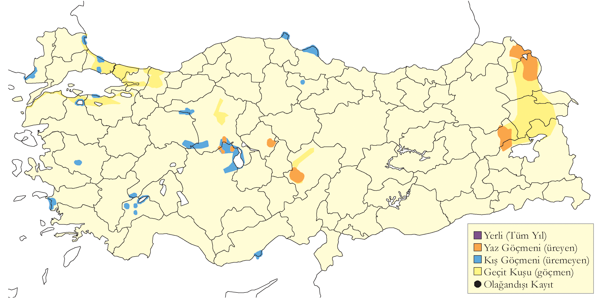
\includegraphics{images/harita_Page_002.png}

\textbf{Üreme}

\textbf{Yuvalama alanı:} Göllerdeki adalarda genellikle küçük gruplar
halinde ürer.\\
\textbf{Yuvası}: Kulu Gölü'nde gözlenen yuvası kuru toprağa kazılmış sığ
bir çukurdur ve çevredeki bitki örtüsü ve küçük tüylerle astarlanmıştır.
Ereğli Sazlığı'ndaki yuvası saz ve diğer sucul bitkilerden oluşan ve su
seviyesinin üstünde kalan bir yapının üzerine kurmuştur.\\
\textbf{Yumurta sayısı:} Türkiye'de yumurta sayısına ilişkin güvenilir
gözlem yoktur. Yuvadan ayrılmış beş kaz yavrusu, görülen en kalabalık
gruptur. Diğer ülkelerde genellikle 4-6 yumurta koyar.\\
\textbf{Üreme dönemi:} Mart sonunda yumurta koyar. En erken yavrular 23
Nisan 1988'de Kulu Gölü'nde, 27 Nisan 1988'de Sultansazlığı'nda, 30
Nisan 1968'de Mogan Gölü'nde ve 30 Nisan 1973'de Ereğli Sazlıkları'nda
gözlenmiştir. 20 Nisan 1996'da Marmara'da, 14 Mayıs 1969'ta
Karadeniz'de, 16 Mayıs 1970'da ve 24 Haziran 1983'te Doğu Anadolu'da
kaydedilen yavrular gecikmiş üremeyi gösterir.

\textbf{Alttürler ve Sınıflandırma}

Ülkemizde \emph{rubrirostris} alttürü bulunur. Bu alttür turuncu
gagasıyla Batı ve Orta Avrupa'da bulunan pembe gagalı \emph{anser}
alttüründen ayrılır.

\section{Sakarca}\label{sakarca}

\emph{Anser albifrons}, Greater White-fronted Goose

\textbf{\emph{Lokal olarak bulunan ve zaman zaman kalabalık sürüler
oluşturan bir kış konuğudur.}}

Ekim sonu ile nisan başı arasında lokal olarak görülen bir kış
konuğudur. Genellikle ocak ve şubat ayında daha yaygın ve yüksek sayıda
olur. Soğuk geçen kışlar Türkiye'de kışlayan nüfusu artar. En kalabalık
sürüler Meriç Nehri boyunda, Tuz Gölü çevresinde ve Konya Ovasında
yoğunlaşır. Büyük Menderes Deltası ve Doğu Akdeniz sulakalanlarında
önemli sayılarda toplanabilir. Son zamanlarda Güneydoğu Anadolu'daki
baraj göllerinde küçük sürüler halinde görülmeye başlamıştır. Nadiren
yazın sulakalanlarda az sayıda kalabilir.

Kış ortası su kuşu sayımlarında (KOSKS) ülke genelinde en yüksek sayıda
1968-69 kışında 98.600 birey sayılmıştır. 1987'de toplam 84.000 birey
kaydedilmiştir. Daha sonra kışlayan sayılar ciddi bir düşüş yaşamıştır.
1990'lı yıllarda genellikle 20.000-30.000, 1993'de
11.822\textsuperscript{12}, 1999'da 3956\textsuperscript{13} ve 2005'te
3891 birey\textsuperscript{14} tespit edilmiştir. Kışın soğuk geçtiği 11
Şubat 2006'de Büyükçekmece'de sayılan 15.000 birey son yıllardaki en
yüksek sayımdır. Dolayısıyla, Türkiy'de kışlayan nüfusun 1970'lerde
100.000'ler seviyesinden 2010'larda 5000 seviyesine indiği tespit
edilmiştir.

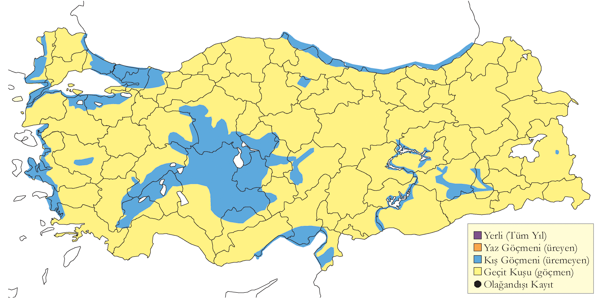
\includegraphics{images/harita_Page_003.png}

\textbf{Üreme}

Türkiye'de yuvalamaz. Avrasya ve Kuzey Amerika'nın tundra bölgelerinde
yuvalar.

\textbf{Alttürler ve Sınıflandırma}

Türkiye'de nominat alttürü bulunur.

\section{Küçük Sakarca}\label{kuxfcuxe7uxfck-sakarca}

\emph{Anser erythropus}, Lesser White-fronted Goose

\textbf{\emph{Az sayıda gelen düzenli kış konuğudur.}}

Her yıl çok az sayıda kaydedilen bir kış konuğudur. Hiçbir alanda
düzenli olarak bulunmadığı düşünülür. Sayıları genellikle 10'dan azdır.
Çoğunlukla diğer kaz türleri ile karışık olarak bulunur. Bugüne kadar,
Türkiye'ye gelen bireylerin İskandinavya'da üreyen ve Balkan ülkelerinde
kışlayan göçyolu (flyway) nüfusuna ait olduğu düşünüldü. Yunanistan'da
bir alanda kışlayan ve koruma çalışmaları nedeniyle sayıları artan
sürünün kış ortasında oradan kaybolması, Marmara ve Ege bölgelerinde bir
kışlama alanının ihtimalini doğurdu. Ancak yapılan aramalara rağmen
burada düzenli ziyaret edilen bir kışlama alanı bulunamadı.

Ülkenin diğer ucunda, 20 Kasım 2004'te Haçlı Gölünde uydudan izlenen bir
birey sinyal verince, doğuda bir kışlama alanın ihtimali
doğdu\textsuperscript{15}. Nitekim Van Gölü ve Erçek Gölü kıyılarında
sayıları 340'ı bulan kalabalık sürüler düzenli olarak tespit edildi.
Bugün ülkede kışlayan ana nüfusun Doğu Anadolu'da bulunduğu
söylenebilir\textsuperscript{16}.

2000 öncesindeki kayıtlara bakıldığında; 29 Aralık 1997'de Göksü
Deltası'nda bir birey\textsuperscript{6}, 23 Ocak 1993'te Göksu
Deltası'nda bir birey\textsuperscript{12}, 6 Nisan 1990'da Seyfe
Gölü'nde 12 birey\textsuperscript{9}, 24 Aralık 1986'da Bafa Gölü'nde
bir erişkin iki genç\textsuperscript{17} ve 16 Şubat 1967'da Kocabaş
Çayının ağzında (Çanakkale) iki birey\textsuperscript{1} kaydedilmiştir.
1945 ile 1965 ve ekim ile ocak arasında büyük çoğunluğu Büyükçekmece ve
Küçükçekmece göllerinden gelen 12 kaydı vardır. Ancak bu kayıtlar tür
tanımını destekleyecek belgeden yoksundur\textsuperscript{18}.

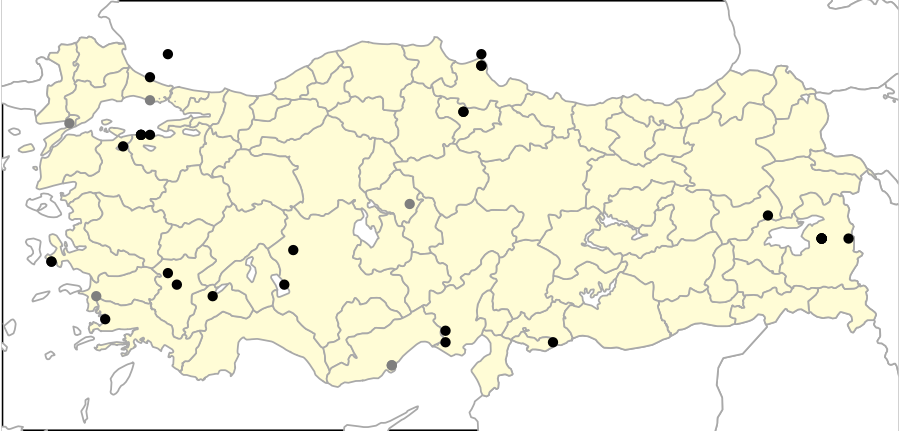
\includegraphics[width=6.25in,height=\textheight]{images/harita_Anser_erythropus.png}

\textbf{Üreme}

Türkiye'de yuvalamaz. Kuzey İskandinavya'dan Doğu Sibirya'ya uzanan
tundra kuşağında ürer.

\textbf{Alttürler ve Sınıflandırma}

Monotipik bir türdür.

\section{Tundra Kazı}\label{tundra-kazux131}

\emph{Anser serrirostris}, Tundra Bean Goose

\textbf{\emph{Nadiren gelen kış konuğudur.}}

2000 yılından sonra üç kere kaydedilmiştir. Birer birey 26 Şubat 2013'te
Yedikır Barajı'nda, 4-21 Şubat 2015'te Kızılırmak Deltası'nda ve Manyas
Gölü'nde 2 birey görülmüştür. Tür kış aylarında sakarca sürüleri
arasında bulunabilir.

Tundra Kazı, önceleri Tayga Kazı ile beraber tek bir tür altında Tarla
Kazı olarak sınıflandırılırdı. Dolayısıyla, taksonomik revizyonun
yapıldığı tarihin öncesindeki kayıtlarda Tarla Kazı olarak
tanımlanmıştır. 2000'den sonra çekilen fotoğraflarda özellikle gaga
renklenmesi incelenmiş, bu kuşların hepsi Tundra Kazı olarak
tanımlanmıştır. Fotoğrafı veya betimlemesi olmayan eski kayıtların hangi
türe ait olduğu belirsiz kalacaktır.

Tarla Kazı olarak tanımlanmış kuşlar Ege, Akdeniz ve İç Anadolu'daki
sulakalanlarda ara sıra yüksek sayılarda kaydedilmiştir. 1870'ler ve
1880'lerde Mersin'de toplanan bireyler\textsuperscript{19} ilk
kayıtlarıdır. 1966-2000 arasında çoğunlukla ocak ile mart arasında 15
kez kaydedilmiştir. 2 Mart 1965'te Ereğli ve Karapınar arasında 90
birey\textsuperscript{18}, 15-16 Ekim 1969'da Karamık Sazlıklarında 13
birey\textsuperscript{2}, 30 Nisan 1988'de Seyfe Gölü'nde, 30 Ocak
1992'de Marmara Gölü'nde 61 birey, 9 Ocak 1993'te Büyükçekmece Gölü'nde
64 birey\textsuperscript{12} ve 24 Ocak 1993'te Göksu Deltası'nda bir
birey\textsuperscript{12} kaydedilmiştir. Türkiye'deki kışlayan Sakarca
sayılarındaki sert düşüş muhtemelen Tarla Kazı olarak tanımlanmış kuşlar
için de geçerlidir.

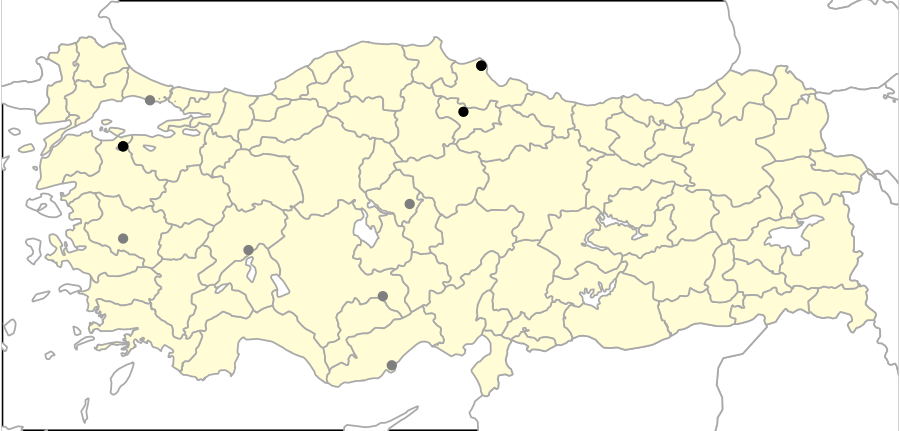
\includegraphics[width=6.25in,height=\textheight]{images/harita_Anser_serrirostris.png}

\textbf{Üreme}

Türkiye'de yuvalamaz. Üreme alanı Kuzey İskandinavya'dan Doğu Sibirya'ya
uzanan tundra kuşağındadır.

\textbf{Alttürler ve Sınıflandırma}

Tayga Kazı yeni bir türdür ve yakın zamana kadar Tarla Kazı olaran
bilinen bir türden ayrılmıştır. 5 alttürden oluşan Tarla Kazı
(\emph{Anser fabalis}) ikiye ayrılınca \emph{fabalis}, \emph{johanseni}
ve \emph{middendorffii} alttürleri Tayga Kazı (\emph{Anser fabalis}),
\emph{serrirostris} ve \emph{rossicus} alttürleri Tundra Kazı
(\emph{Anser serrirostris}) altında sınıflandırılmıştır.

\section{Yosun Kazı}\label{yosun-kazux131}

\emph{Branta bernicla}, Brant Goose

\textbf{\emph{Rastlantısal konuktur.}}

Batı Avrupa'da Atlantik kıyılarında kışlayan bir türdür. Türkiye ve
yakın coğrafyasında rastlantısal konuktur. 6 Nisan 1981'de Küçük
Menderes Deltası'nda iki birey\textsuperscript{5}, 3-4 Eylül 1973'te
Ardeşen açıklarında koyu karınlı \emph{bernicla} alttürüne ait iki birey
kaydedilmiştir\textsuperscript{3}. 1969 yılında Acıgöl'den gelen bir
iddia kabul edilmemiştir\textsuperscript{20}. 7 Şubat 1945'de
Büyükçekmece'de bir bireyi Prenses Zeyneb Halim vurmuştur, maalesef bu
kuşun gövdesi korunamamıştır\textsuperscript{18}. Kışın soğuk geçtiği
Ocak 1889'da düzenli olarak İstanbul Maltepe'de ve Şubat 1891'de büyük
sürüler halinde İstanbul Kadıköy'de görülmüştür\textsuperscript{21}.

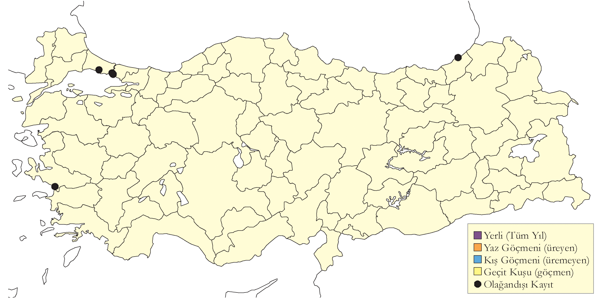
\includegraphics{images/harita_Page_005.png}

\textbf{Üreme}

Türkiye'de yuvalamaz. Orta ve Kuzey Sibirya'da Kuzey Kutup Denizi kıyı
şeridinde yuvalar.

\textbf{Alttürler ve Sınıflandırma}

Bir kayıtta \emph{bernicla} alttürü tanımlanmıştır. Kuzeybatı Avrupa'da
kışlayan \emph{bernicla} alttürünün Türkiye'de görülmesi makuldür.
Yunanistan'daki bir kaydı da bu alttüre aittir\textsuperscript{22}.

\section{Ak Yanaklı Kaz}\label{ak-yanaklux131-kaz}

\emph{Branta leucopsis}, Barnacle Goose

\textbf{\emph{Rastlantısal konuktur.}}

5 Ocak 2003'te Büyükçekmece Gölü'nde bir birey gözlenmiş ve detaylı
olarak belgelenmiştir. 1946/47 kışında Sakarya Deltası'nda bir birey,
1961 sonbahar/kışında diğer bir birey vurulmuş, ikinci kuşun tahniti
Eylül 1964'de Ankara'ya bulunmuş, ancak sahibi satmayı
reddetmiştir\textsuperscript{23}. Bu iki kaydın dökümantasyonu
yetersizdir\textsuperscript{18}.

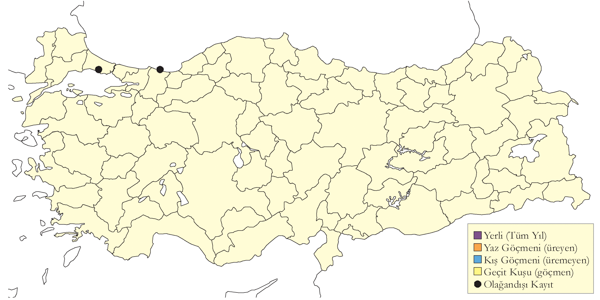
\includegraphics{images/harita_Page_006.png}

\textbf{Üreme}

Türkiye'de yuvalamaz. Grönland, İzlanda, Kuzey Batı Rusya ve Baltık
Denizi kıyılarında yuvalar.

\textbf{Alttürler ve Sınıflandırma}

Monotipik bir türdür.

\section{Sibirya Kazı}\label{sibirya-kazux131}

\emph{Branta ruficollis}, Red-breasted Goose

\textbf{\emph{Az sayıda gelen düzensiz kış konuğudur.}}

Özellikle soğuk kışlarda bazı bireyler veya gruplar Türkiye'ye inerler
ve düzensiz olarak görülürler. Türkiye'de düzenli kışladığı bir alan
yoktur. Ana kışlama alanı Romanya ve Bulgaristan'ın Karadeniz kıyı
şerididir. 1964 ila 2008 arasında 64 kaydı bilinir. Bu kayıtların
Marmarada 15 kayıt, İç Anadolu'da 12 kayıt, Karadeniz'de 8 kayıt,
Akdeniz'de 6 kayıt ve Ege'de 4 kayıt alınmıştır. Kayıtların çoğu aralık
sonu ile şubat başı arasından gelir. Bu kayıtların çoğunda bir veya
birkaç kuş sayılmışi ancak 5 tanesinde 40 ila 100 bireylik kalabalık
sürüler de gözlenmiştir. 2001/2002 kışında ülke toplamında 192 birey
sayılmıştır.

Ülke genelinde yaygın olarak av mağazaları ve avcılık kulüplerinde
tahnitlerine rastlanması ve avcıların gözlem
beyanları\textsuperscript{24} kayıtların işaret ettiğinden çok yaygın
olduğunu gösterir. İç Anadolu'dan gelen eski kayıtlar, Kış Ortası Su Kuş
Sayımlarında kalabalık kaz sürülerinin sistematik incelenmesi ile ortaya
çıkmıştır. Sakarca sürülerinin içinde olabilecek bireylerin farkedilmeme
ihtimali yüksektir.

1946/47 kışında Küçükçekme'de Kosswig tarafından
gözlenmiştir\textsuperscript{23}. 1947 veya 1954 yılında kış boyunca (27
Kasım - 6 Mart) Büyükçekmece ve Meriç Nehri (?) arasında düzenli olarak
9 birey ve Beylik Mandra'da 2 birey kaydedilmiştir\textsuperscript{18}.
1959 yılında belirtilmemiş bir alanda sekiz İshakoğlu tarafından birey
gözlenmiş ve bir birey vurulmuştur\textsuperscript{25}. 12 Kasım 1964'de
Kuyucuk Gölü'nde 2 erişkin ve bir genç birey 400 boz kazın arasında
kaydedilmiştir\textsuperscript{26}. 17 Ocak 1965 tarihinde Çekmece'de E.
Hirzel tarafından üç birey görülmüştür.

Türkiye'den açıklamaya ihtiyaç duyulan bir yaz veya üreme kaydı vardır.
5 Ağustos 1982'de Erçek Gölü'nde 14 erişkin ve sekiz yavru
kaydedilmiştir\textsuperscript{27}. Bu kayıt ya hatalı bir kayıt olarak
unutulmalı, ya da avcılar tarafından yakalanmış ve evcilleştirilmiş
kuşların üretilmesinin bir sonucu olarak yorumlanmalıdır.

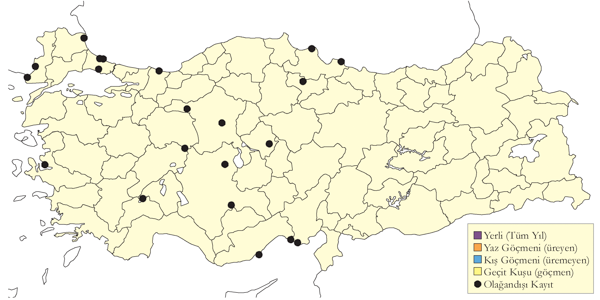
\includegraphics{images/harita_Page_007.png}

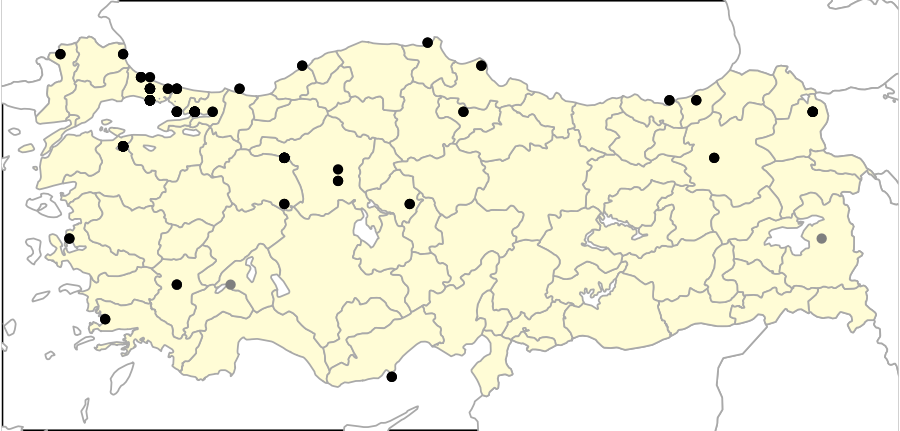
\includegraphics[width=6.25in,height=\textheight]{images/harita_Branta_ruficollis.png}

\textbf{Üreme}

Türkiye'de yuvalamaz. Doğu Sibirya'da tundra kuşağında yuvalar.

\textbf{Alttürler ve Sınıflandırma}

Monotipik bir türdür.

\section{Sessiz Kuğu}\label{sessiz-kuux11fu}

\emph{Cygnus olor}, Mute Swan

\textbf{\emph{Lokal olarak az sayıda yuvalar. Yaygın olarak ve nispeten
çok sayıda bulunan bir kış konuğudur.}}

Üreme kayıtlarının çoğu 3 alandan gelir: Gala Gölü, Gediz Deltası ve
Kızılırmak Deltası. Ulusal üreme popülasyonu muhtemelen 20 çiftten daha
azdır. Kızılırmak Deltası'ndan ilk muhtemel üreme kaydı 1968 yılında
alınmıştır\textsuperscript{24}.

Geçmişte birkaç alanda üreyen yüzlerce çiftlik bir nüfus bulunuyordu.
Marmara Gölü'nde 50 çift, Akşehir Gölü'nde 100 çift
üremiştir\textsuperscript{28}. Ereğli Sazlığı en çok gözlem kaydının
alındığı alandır. Lenz burada 1968'de 11 yuva, 1969'da bir yuva ve
1970'de üç yuva bulmuştur. Buradaki sulakalanın yokolması ayrıntılı
olarak belgelendiği için\textsuperscript{29}, üreyen nüfusun azalışı da
gözlenmiştir. Eski üreme alanlarında yok olmasının ana nedeni
sulakalanların kurutulmasıdır.

Kışın Karadeniz ve Marmara ve Ege Bölgesinde yaygın olarak en yüksek
sayılarda gözlenir. Toplam kışlama popülasyonu 1000-10000 birey
arasındadır. Meriç Deltası ve Gala Gölü ülke nüfusunun çoğunun
toplandığı alandır, burada 1993'de 1244 birey\textsuperscript{12}
1999'da 8900 birey\textsuperscript{13} ve 2003'te 2000 birey
sayılmıştır. Kışın sert geçtiği yıllarda sayısı artar, 1999'da ülke
toplamında 9088 birey kaydedilmiştir.

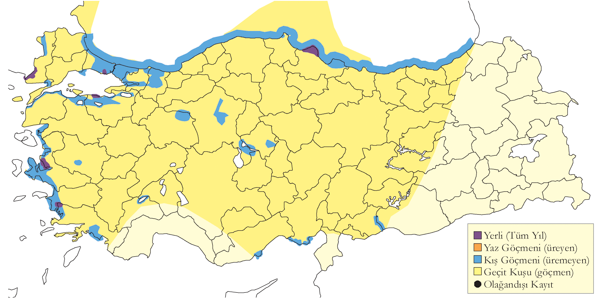
\includegraphics{images/harita_Page_008.png}

\textbf{Üreme}

\textbf{Yuvalama alanı:} Geniş sazlık alanlar ve göl açıklığı bulunan
büyük göller ve bataklıklardır.\\
\textbf{Yuvası:} Türkiye'deki bir yuvanın tarifi yapılmamıştır. Diğer
yerlerde yuva su kenarında zemin üzerinde, küçük bir adacıkta veya sığ
sudaki sazların üstüne kurulur. Yuva saz ve diğer sucul bitkilerden
oluşan büyük bir yığının ortasındaki çukura kurulur.\\
\textbf{Yumurta sayısı:} Türkiye'de yumurta gözlemi yoktur. Türkiye
dışında 5-7 yumurta koyduğu bilinir.\\
\textbf{Üreme dönemi:} Nisan başında yumurta koyar, mayıs ve temmuz
arasında yavrular gözükür. 13 Mayıs 1899'da İzmir'de saz yatağında
yuvalan bir çift kaydedilmiştir\textsuperscript{30}. 6 Temmuz 1976'da
Ereğli Sazlığında bir çift ve 4-5 genç yavru, 17 Temmuz 1982'de bir çift
ve dört genç ve 16 Mayıs 1987'de yumurtadan yeni çıkmış yavrular
gözlenmiştir.

\textbf{Alttürler ve Sınıflandırma}

Monotipik bir türdür.

\section{Küçük Kuğu}\label{kuxfcuxe7uxfck-kuux11fu}

\emph{Cygnus columbianus}, Tundra Swan

\textbf{\emph{Lokal olarak ve az sayıda bulunan bir kış konuğudur.}}

1993 yılına kadar nadir bir kış konuğu olduğu düşünülmüştür. Daha sonra
ilk önce Burdur Gölü ve Göller bölgesinde, ardından Meriç Deltası düzenl
bulunduğu tespit edilmiştir. Meriç Deltası'nda karışık ve kalabalık kuğu
sürüleri içinde sayıları 1000'e ulaşabilir. İç Anadolu, Göller
Bölgesi'nda küçük gruplar halinde bulunur. Ekseriyetle kasım ve nisan
arasında bulunur.

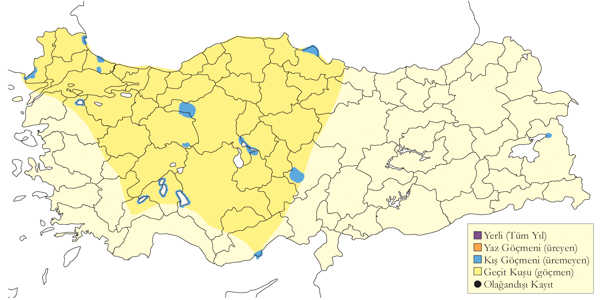
\includegraphics{images/harita_Page_009.png}

\textbf{Üreme}

Türkiye'de yuvalamaz. Türkiye'de kışlayan kuşların üreleme alanının ve
göç koridorları tespit edilmiştir\textsuperscript{31}. GPS ve GMS
vericileri ile 2015-2017 yılında yapılan çalışmada yuvalama alanlarının
Yamalo-Nenets özrek bölgesindeki Yamal olduğu, göçleri sırasında Ob
Koyu, Turgay Ovaları, Kuzey Hazar Kıyıları, Azov Denizi gibi durak
alanlar üzerinden göç ettikleri ortaya çıkmıştır.

\textbf{Alttürler ve Sınıflandırma}

Ülkemizde Eski Dünya'da yaşayan \emph{bewickii} alttürü bulunur ve gaga
kökü ve yüz derisi sarıdır. Amerika'da yaşayan \emph{columbianus}
alttürü siyah gaga ve siyah yüz derisi ile kolaylıkla ayırt edilebilir.

\section{Ötücü Kuğu}\label{uxf6tuxfccuxfc-kuux11fu}

\emph{Cygnus cygnus}, Whooper Swan

\textbf{\emph{Yaygın olarak ve az sayıda görülen bir kış konuğudur.}}

Ekim sonu ve nisan başı arasında yaygın olarak az sayıda görülen bir kış
konuğudur. Ocak ve şubat aylarında en yüksek sayıya ulaşır. Trakya'da
Meriç Deltası ana toplama bölgesi ve türün Balkanlar'daki en önemli
kışlama alanıdır. 25 Ocak 1998'de bulunan 1200 birey Türkiye'deki en
yüksek sayıdır.\textsuperscript{32} Türkiye'ye gelen kuşlar Ukrayna ve
Kırım ile Batı Karadeniz Bölgesi arasındaki deniz üzeri göç rotasını
kullanır\textsuperscript{33}. Doğuda 30 Ekim 1995'de Sodalı Gölü'nde 164
birey\textsuperscript{34}, 1992'de Diyarbakır Kabaklı Barajı'nda 133
birey\textsuperscript{35} kaydedilmiştir.

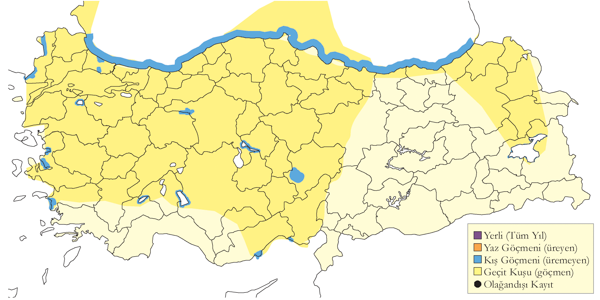
\includegraphics{images/harita_Page_010.png}

\textbf{Üreme}

Türkiye'de yuvalamaz. Avrasya'nın kuzeyinde yuvalar.

\textbf{Alttürler ve Sınıflandırma}

Monotipik bir türdür.

\section{Nil Kazı}\label{nil-kazux131}

\emph{Alopochen aegyptiaca}, Egyptian Goose

\textbf{\emph{Durumu belirsizdir. Çoğunlukla egzotik tür kategorisinde
değerlendirilir.}}

28 Nisan 1986'da Kulu Gölü'nde bir birey gözlenmiş, kuşun doğal ve
rastlantısal konuk olduğu düşünülmüştür. 11 Nisan 1911'de Urfa'nın
güneyinde iki birey gördüğünü söyleyen Weigold'un (1912-13) kaydı ise
kabul görmemiştir\textsuperscript{36}.

İstanbul ve Ankara'da gözlenen kuşların esaretten kaçtığı düşünülür.
6-13 Temmuz 2002'de Ankara'daki bir parkta bir çift fotoğraflanmış, 31
Mart 2012'de İstanbul Riva'da bir çift, 13 Mart 2012'de Ankara Hacettepe
Kampüsü'nde, 5-24 Kasım 2013'de Etimesgut'ta ve 25 Mayıs-13 Haziran
2014'da Eymir Gölü'nde birer birey gözlenmiştir.

1906 ve 1928 arasında Kıbrıs'ta nadir rastlanan bir kış göçmeni olarak
değerlendirilmiş, 1958, 1962 ve 1989 yıllarında bireyler gözlenmiştir.
Eskiden Suriye ve Filistin'de ürediğini düşünülmüş\textsuperscript{37},
sonrasında Suriye'de hiçbir güvenilir kaydı olmadığına karar
kılınmıştır\textsuperscript{38,39}.

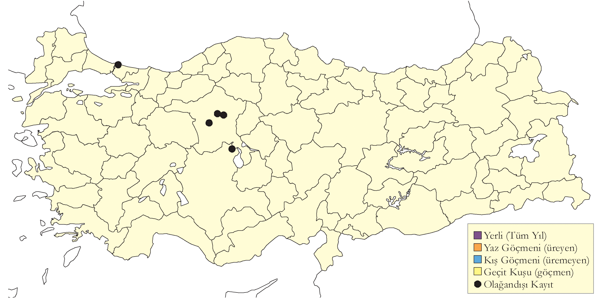
\includegraphics{images/harita_Page_011.png}

\textbf{Üreme}

Türkiye'de yuvalamaz. Afrika'da çoğunlukla Sahra Altında yuvalar.

\textbf{Alttürler ve Sınıflandırma}

Monotipik bir türdür.

\section{Suna}\label{suna}

\emph{Tadorna tadorna}, Common Shelduck

\textbf{\emph{Lokal olarak az sayıda ürer. Lokal olarak çok sayıda
bulunabilen bir kış konuğudur.}}

Ege Bölgesi, Göller Bölgesi, İç ve Doğu Anadolu'da geniş ve tuzlu
sulakalanlarda ürer. Başlıca üreme alanları Gediz Deltası, Bolluk, Kulu
ve Tuz Gölleri ve Van Gölü çevresidir. Gediz Deltası'nda 1996 yılında
üreyen popülasyonun 8 çift olduğu tahmin edilmiş\textsuperscript{40}. 24
Haziran 1992'de Bolluk Gölü'ndeki bir adada 12 yuva bulunmuştur.

Üreme sonrası tüy değiştiren kuşlar ağustos-ekim arasında toplanırlar,
Erçek Gölü'nde 2500 birey, Kulu Gölü'nde 700 birey sayılmıştır.

Kışlayan toplam nüfus genellikle 1000-5000 bireydir, ana kışlama alanı
Yumurtalık Lagünü'nde 16 Şubat 2006'da 5390 birey sayılmıştır. Acıgöl'de
1969-70'de 3450 birey, 1968-69'da 4900 birey, 2004'te 1802 birey ve
2005'te 2928 birey sayılmıştır. Diğer alanlarda daha küçük topluluklar
oluşturur.

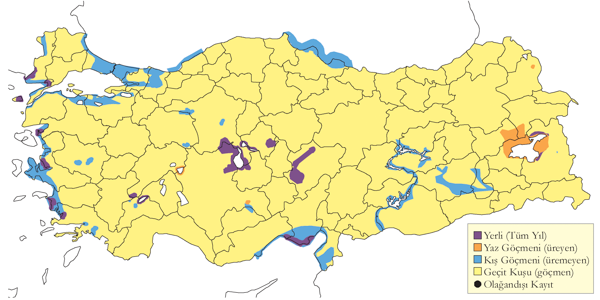
\includegraphics{images/harita_Page_012.png}

\textbf{Üreme}

\textbf{Yuvalama alanı:} Geniş, sığ ve tuzlu sulakalanlarda adalar,
sedde duvarları ve çalı altlarında yuvalar.\\
\textbf{Yuvası}: Avrupa'da yuvaların çoğu tavşan oyuklarında, tünelin
1-2 m içinde bulunur. Buna karşın Türkiye'deki yuvalar yerdedir. Bolluk
Gölü'ndeki yuvaların bazıları tamamen açıkta, bazıları kısmen ya da
tamamen çalı altında ve bir tanesi doğal bir oyuğun içinde
bulunmuştur.\\
\textbf{Yumurta sayısı:} 6-9 yumurta koyduğu gözlenmiştir. Bolluk
Gölü'ndeki yuvalarda gözlenen 10-18 yumurtanın birden çok dişi
tarafından konulmuş olması muhtemeldir.\\
\textbf{Üreme dönemi:} Gediz Deltasında haziran başında yavrular
görülmüştür\textsuperscript{40}. İç Anadolu'da nisan sonu ile haziran
başında yuvalar. Doğu Anadolu'da haziran ortasında yumurtladığı
düşünülmektedir.

\textbf{Alttürler ve Sınıflandırma}

Monotipik bir türdür.

\section{Angıt}\label{angux131t}

\emph{Tadorna ferruginea}, Ruddy Shelduck

\textbf{\emph{Yaygın ve çok sayıda bulunan yerli türdür. Kışın göç alır,
sayıları artar.}}

Üremek için Genellikle yüksek kesimlerdeki küçük gölcükler, baraj
gölleri, ıslak çayırlar ve dereleri seçer, birçok ördek ve kaz türünün
aksine büyük sulakalanlarda bulunmaz. İlk tahminde üreyen popülasyonun
4000 ile 8000 çift arasında olduğu öne sürmüştür\textsuperscript{41}.
Sonrasında kış ortası su kuşu sayımlarına dayanarak azaldığı
düşünülmüştür. Üreyen popülasyonun 1200-5100 çift olduğunu tahmin
etmiştir\textsuperscript{42}.

Temmuz eylül arasında tüy değişimi için bazı sulakalanlarda büyük
sürüler halinde toplanır. Erçek Gölü'nde 20.000 birey, Sultan
Sazlığı'nda 11.000 birey, Kulu Gölü'nde 10.000 birey, Eylül 1936'da
bugün kurutulmuş olan Emir Gölü'nde 10.000-15.000 birey sayılmıştır. Kış
öncesinde Kasım 2004'de Sarıyar Barajı'nda 8.000 birey ve Kuyucuk
Gölü'nde 6.000 birey kaydedilmiştir.

Kış aylarında daha yaygın olarak görülür. En yüksek kış sayımında ülke
toplamında 10.115 birey\textsuperscript{14}, genellikle 4000-4500 birey
sayılmıştır. Ocak-Şubat 1993'te sadece 711 birey, sadece Sarıyar
Barajı'nda 18 Ocak 2004'te 5636 birey ve 18 Şubat 2006'da 7641 birey
kaydedilmiştir. Bir yandan İç Anadolu'da üreme sonrası toplanan
sürülerde bir azalma görülmüş, diğer yandan baraj göllerinin sayısındaki
artış gözlenmiştir. Kış sayımı toplamlarının yaz sonu toplamlarından az
olması, dağınık şekilde kışladığına veya kış ayında güneye göç vermesine
bağlanabilir. Toplam kışlayan nüfusun 2600 ile 28.500 birey arasında
değiştiği düşünülmüştür\textsuperscript{42}.

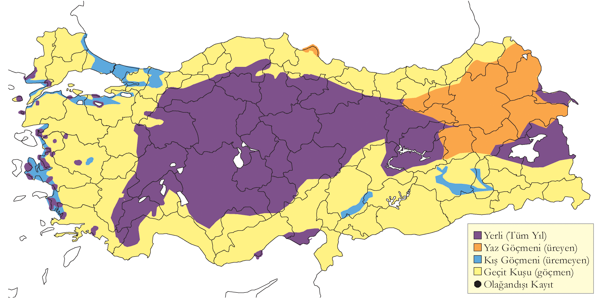
\includegraphics{images/harita_Page_013.png}

\textbf{Üreme}

\textbf{Yuvalama alanı:} Genellikle göl kenarlarındaki sarp kayalıklarda
ve tepelerde, yamaçlardaki çukur ve çatlaklarda olmak üzere açık
alanlarda ürer. Sıkça kayalıklarda yuvalar. Beyşehir Gölü'ndeki bir
adada kayaların ve harabelerin taşları arasında ürediği kaydedilmiştir.
22-24 Mayıs 1998'de Ereğli yakınlarındaki bir kayalıkta muhtemelen eski
bir Kızıl Şahin yuvasında kuluçkaya yatmış bir dişi gözlenmiştir.\\
\textbf{Yuvası}: Yuvası Türkiye'de tanımlanmamıştır, genellikle bitki
artıkları, hav tüyleri ve bazı diğer tüylerle kaplanmış bir oyuktur. 30
Nisan 2003'te Akköy yakınındaki dik bir yamaçtaki muhtemelen bir tavşan
yuvası olan oyuğa giren bir dişi gözlenmiş, ancak oyuğun derin olması
nedeniyle yuva incelenememiştir.\\
\textbf{Yumurta sayısı:} 8-12 yumurta koyduğu görülmüştür.\\
\textbf{Üreme dönemi:} Akdeniz ve Ege'de mart sonu yumurta koyar.
Kuluçka diğer bölgelerde nisan ve mayıs arasında başlar.

\textbf{Alttürler ve Sınıflandırma}

Monotipik bir türdür.

\section{Boz Ördek}\label{boz-uxf6rdek}

\emph{Mareca strepera}, Gadwall

\textbf{Lokal olarak birkaç alanda yuvalar. Yaygın olarak orta sayılarda
bir kış konuğudur.}

En önemli üreme alanı Kızılırmak Deltası'nda 200 çift ürer. Türkiye'de
toplam üreyen popülasyonun 500 ile 5000 çift arasında olduğu
düşünmüştür\textsuperscript{41}. Bugüne gelindiğinde sayılarının
azaldığı ortadadır.

İç Anadolu'daki ilkbahar geçişi marttan nisan başına kadar belirgindir.
Akdeniz'deki kıyısal sulakalanlarda nadiren 1000'den yüksek sayılarda
gözlenir. Kış ortası sayımlarda 1967'de Manyas Gölü'nde 5000 birey,
1969'da Akşehir Gölü'nde 7500 birey ve 1971'de Hotamış Sazlığı'nda 2490
birey sayılmıştır. 1967-73 arasında ülke genelinde çoğunlukla 3000'den
fazla kaydedilmiştir. 1986-2005 arasında toplam sayı 1000-1500
seviyesine düşmüş, son yıllarda tekrar artmış, 2020 kışında Kızılırmak
Deltası'nda 10.000 bireyden fazla sayılmıştır.

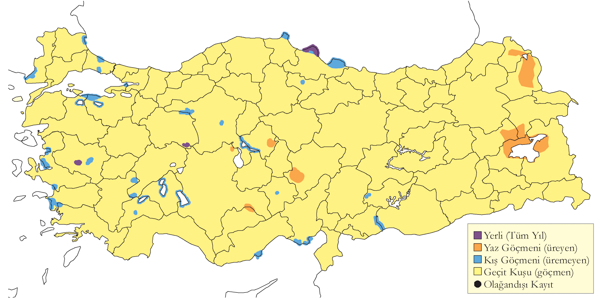
\includegraphics{images/harita_Page_014.png}

\textbf{Üreme}

\textbf{Yuvalama alanı:} Göl kıyılarında ve adalarındaki yoğun
vejetasyon içinde; sazlıklarda ve sık bitkilerle kaplı taşkın
alanlarında ürer. Kızılırmak Deltası, Karamık Gölü, Kulu Gölü, Bolluk
Gölü, Mogan Gölü, Ahlat Sazlıkları, Haçlı Gölü ve Van Gölü'nde
yuvalamıştır.\\
\textbf{Yuvası:} Yuva yerde bir çukura kurulur, bitkisel malzeme ve
dişinin tüyleriyle kaplanır. \textbf{\hfill\break
Yumurta sayısı:} Türkiye'deki yuvalarda yumurta sayısı 6-15 arasındadır.
İç Anadolu'da 7-15 yumurtalı yuvalar görülmüş, bu yumurtaların 1 ila 6
tanesi başka ördeklerin koymuş olduğu tespit edilmiştir. Kulu Gölü'ndeki
yuvalarda 6 Mayıs 1972'de 3-11 yumurta ve 14 Temmuz 1971'de 7 yumurta
sayılmıştır\textsuperscript{43}. 17 Mayıs 2004'te Bolluk Gölü'ndeki bir
yuvada 8 yumurta bulunmuştur.\\
\textbf{Üreme dönemi:} Kızılırmak Deltası'nda nisan başında yumurta
koyar\textsuperscript{44}. İç Anadolu'da nisan sonu ile temmuz arasında,
Doğu Anadolu'da haziran ile eylül arasında yavrulara rastlanmıştır.

\textbf{Alttürler ve Sınıflandırma}

Türkiye'de nominat alttürü bulunur. Eskiden \emph{Anas} cinsi altında
sınıflandırılırdı.

\section{Fiyu}\label{fiyu}

\emph{Mareca penelope}, Eurasian Wigeon

\textbf{\emph{Yaygın olarak çok sayıda bulunan kış konuğu ve geçit
türüdür.}}

Ege, Akdeniz ve İç Anadolu'nun sulakalanlarında kalabalık sürüler
halinde kışlar. 1960'lı ve 70'li yıllarda düzenli olarak ortalama
150.000 birey sayılmıştır. En yüksek sayıda 1968'de 208.600 birey,
1969'da 458.800 birey kaydedilmiştir. Bugünlere gelindiğinde ciddi bir
düşüş yaşamıştır. 1986 ile 2005 arasındaki düzenli sayımlarda sadece
dört yıl 40.000'dan fazla birey kaydedilmiştir. Çoğunlukla eylül sonunda
gelir, nisan sonuna kadar kalır.

İç Anadolu'da mart sonu ve nisan başı arasında yüksek sayıda geçer. Bazı
göçmenler mayıs sonuna kadar kalır. Nadiren Doğu Anadolu'da ve
muhtemelen İç Anadolu'da üremeden yazı geçirebilir.

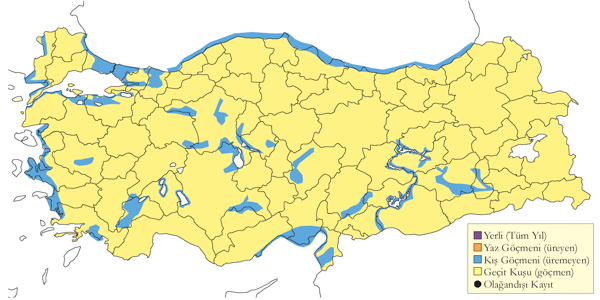
\includegraphics{images/harita_Page_015.png}

\textbf{Üreme}

Türkiye'de yuvalamaz. Kuzey Avrupa'da yuvalar.

\textbf{Alttürler ve Sınıflandırma}

Monotipik bir türdür. Eskiden \emph{Anas} cinsi altında
sınıflandırılırdı.

\section{Yeşilbaş}\label{yeux15filbaux15f}

\emph{Anas platyrhynchos}, Mallard

\textbf{\emph{Yaygın olarak üreyen yerli bir türdür. Kışın göç alır,
yüksek sayılara ulaşabilir.}}

Uygun yaşamalanının bulunduğu coğrafyalarda yaygın olarak az sayıda
yuvalar. En yaygın olarak İç Anadolu Bölgesi sulakalanlarında rastlanır,
diğer bölgelerde çok lokal olarak bulunabilir. En yüksek sayıda
yuvaladığı alan 400-600 çiftin kaydedildiği Kızılırmak Deltası
olmuştur\textsuperscript{44}.

Sonbaharda göç alır ves sayıları artar. Kışlayan gruplar nisan başına
kadar kalır. En yüksek sayılarda Karadeniz, Marmara ve Ege sahil
kuşağında kaydedilir. Akdeniz ve İç Anadolu'da nispeten az sayıda,
Güneydoğu Anadolu ve Doğu Anadolu'da az sayıda bulunur. 2000 ve 2020
arasında kışlayan nüfus ortalama 20.000 birey seviyesinde olsa da, kışın
soğuk geçtiği 2005 yılında ülke genelinde toplam 106.140 birey ve
Kızılırmak Deltası'nda 50.000 birey sayılmıştır.

1960 ve 70'li yıllarda kışlayan nüfusun 100.000'ler seviyesinde
olmuştur. 1967'de Kızılırmak Deltası ve Yeşilırmak Deltası'nda yaklaşık
52.000 ve Büyük Menderes Deltası'nda 42.000, 1968'de Manyas ve Uluabat
göllerinde 42.000, 1969'da Büyük Menderes Deltası'nda 80.000, Akyatan
Lagünü'nde 40.000 ve Amik Gölü'nde 30.000, 1970'de Meriç Deltası'nda
34.500 ve Sultansazlığı'nda 30.000 birey sayılmıştır.

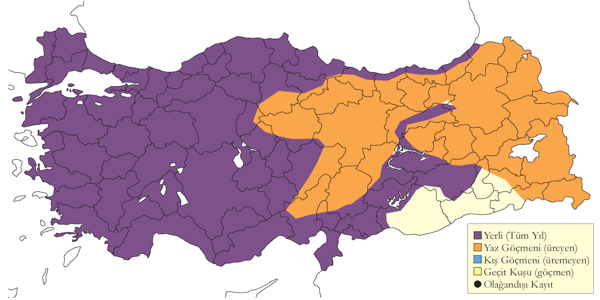
\includegraphics{images/harita_Page_016.png}

\textbf{Üreme}

\textbf{Yuvalama alanı}: Göl ve nehirlerdeki adacıklarda, sazlıklarda,
veya göl, sazlık veya subasar çayırların kıyılarındaki sık bitkilerin
içinde ürer.\\
\textbf{Yuvası}: Yuvasını genellikle bitki örtüsünün altına, topraktaki
bir oyuğa kurar. Başka bölgelerde ağaç kovuğuna yuvaladığı veya
ağaçtaki, örneğin karga gibi, bir kuş yuvasını kullandığı bilinir. Bu
tip yuvalara Türkiye'de henüz rastlanmamıştır.\\
\textbf{Yumurta sayısı}: Genellikle 5-9 yumurta koyar, ancak yumurta
sayısı 2-14 arasında olabilir. Bir yuvadaki yumurtaların 14'ten fazla
olması, birden fazla dişinin aynı yuvaya yumurtladığını gösterir.\\
\textbf{Üreme dönemi}: Kıyı bölgelerinde marttan itibaren, diğer
bölgelerde nisan veya mayısta yumurtlar. Yavrular mayıs başından temmuz
sonuna kadar görülebilir. \textbf{MAR.} 18 Nisan 1993'te Kocaçay
Deltası'nda yavrularıyla gözlenen bir dişi en erken üreme
kaydıdır\textsuperscript{45}. \textbf{KAR.} 19-20 Mayıs 1992'de Yeniçağa
Gölü'nde hem yuvadaki yumurtalar hem de yavrular gözlenmiştir. 5 Mayıs
1992'de Kızılırmak Deltası'nda ilk yavrular
gözlenmiştir\textsuperscript{44}. 16 Mayıs 1967'de Manyas Gölü'nde dokuz
yumurtalı bir yuva kaydedilmiştir. 20 Haziran 1973'te Trakya'da altı
yavrulu bir dişi gözlenmiştir. \textbf{İÇA.} 1971'de Yarma'daki birçok
yuvada diğer türlerin yumurtalarına rastlanmıştır, örneğin, bir yuvada
17 Yeşilbaş, üç Boz Ördek ve üç Macar Ördeği yumurtası tanınmıştır.
13-15 Temmuz 1971'de Kulu Gölü'nde sekiz yuva incelenmiş, yuvalarda 2-12
sayılmış\textsuperscript{43}, başka bir tarihte mayıs ve haziranda
yumurtalı yuvalar ve mayıs ortasından itibaren yavrular gözlenmiştir.
\textbf{DOA.} En erken kayıt 14 Haziran 1968'de Erçek Gölü'nde
kaydedilen yavrulardır. Aynı yerde, 28 Haziran 1968'de beş ve sekiz
yumurtalı iki yuva bulunmuş\textsuperscript{27} ve 9 Haziran 2001'de
Balık Gölü'nde yumurtalı iki yuva kaydedilmiştir.

\textbf{Alttürler ve Sınıflandırma}

Türkiye'de nominat alttürü bulunur.

\section{Kaşıkgaga}\label{kaux15fux131kgaga}

\emph{Spatula clypeata}, Northern Shoveler

\textbf{\emph{Lokal olarak az sayıda yuvalar. Yaygın olarak çok sayıda
bulunan bir geçit türü ve kış konuğudur.}}

İç Anadolu ve Doğu Anadolu'daki birkaç büyük sulakalanda ve Kızılırmak
Deltası'nda yuvalar\textsuperscript{46}. 1970'lerde Kulu Gölü,
Kızılırmak Deltası bilinen üreme alanlarıdır.

Tüm bölgelerde yaygın ve bol olarak kaydedilen bir geçit türüdür. Göçmen
gruplar ilkbaharda mart başından nisan sonuna kadar ve sonbaharda eylül
ortasından kasım başına kadar zaman zaman yüksek sayılarda görülür.
Eylülde Kulu Gölü'nde 7000 birey, Sultansazlığı'nda 9000 birey, mart
sonunda Kızılırmak Deltası'nda 4500 birey sayılmıştır.

Ülkenin batı ve orta bölgelerinde kışlar. 2000 ile 2020 arasında toplam
kışlayan kuş sayısı çoğunlukla 5000 bireyden az olmuştur, kışın soğuk
geçtiği 2005'te 13.576 birey sayılmıştır. Eskiden daha yüksek sayılar
kışlardı, 1993'te toplam 7898 birey, 1999'da 13.114 birey
kaydedilmiştir. Geçmikteki yüksek sayımları şöyledir; 1967'de Büyük
Menderes Delta'sında 23.000 birey, Kızılırmak Deltası'nda 8000 birey,
1993'te aynı yerde 4564 birey ). 1967-73 yılları arasında İç
Anadolu'daki birçok alanda sayıları 3000'i bulan sürülerin kaydı
kaydedilmiştir.

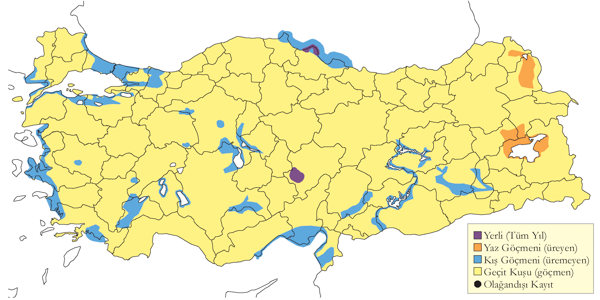
\includegraphics{images/harita_Page_017.png}

\textbf{Üreme}

\textbf{Yuvalama alanı}: Büyük sulakalanlarda yuvalar.\\
\textbf{Yuvası}: Kulu Gölünde bir adadaki cılız vejetasyonun içinde
yuvalamıştır. Çıplak zeminde sığ bir oyuğun içindeki yuva ot ve bitki
gövdeleri ile karışık olarak hav tüyleri ile kaplıdır.\\
\textbf{Yumurta sayısı}: 8-10 yumurta koyduğu kaydedilmiştir.\\
\textbf{Üreme dönemi}: Türkiye'de üremenin sezonu ile ilgili güvenle
yorum yapabilecek yeterli veri yoktur; diğer yerlerde üreme sezonunun
başlaması nisan başından mayıs sonuna kadar değişkenlik gösterebilir.
\textbf{KAR.} 6-7 Temmuz 1972'de Kızılırmak Deltası'nda dört ve beş
yavrulu iki dişi kaydedilmiş\textsuperscript{24}, 1992'de ürediği
kanıtlanamadığı için popülasyonun 0-1 çift olduğu tahmin
edilmiştir\textsuperscript{44}. 1971 Temmuz ortasına ait yumurtalı yuva
kayıtları başarısız bir üremenin ardından ikinci teşebbüs olarak
değerlendirilmelidir. \textbf{İÇA.} 14-15 Temmuz 1971'de Kulu Gölü'ndeki
bir adada sekiz ve on yumurtalı iki yuva bulunmuş, 5-6 Ağustos 1972'de
iki ve dört yavrulu iki yavru grubu görülmüştür\textsuperscript{43}. 31
Mayıs 1987'de Kulu Gölü'nde yavrular gözlenmiş ve 19 Haziran 1992'de
dokuz yumurtalı bir yuva bulunmuştur. Haziran 1977'de Eşmekaya'da beş
yavrusuyla birlikte bir dişi gözlenmiştir\textsuperscript{47}.
\textbf{DOA.} 29 Mayıs 1969'da Van Gölü'nde kur davranışı gözlenmiştir.

\textbf{Alttürler ve Sınıflandırma}

Monotipik bir türdür.

\section{Kılkuyruk}\label{kux131lkuyruk}

\emph{Anas acuta}, Northern Pintail

\textbf{Nispeten yaygın olarak bulunan bir geçit türü ve kış konuğudur.
Nadiren yuvalar.}

Son yıllarda tek bir alanda yuvaladığı bilinir; 1998 ve 1999'da Girdev
Gölü'nde üremiştir. İlkbaharda ve yazın İç Anadolu'da birçok erişkin
kaydı olsa da, kanıtlanmış üreme kayıtları az sayıdadır. Üreyen
popülasyonun 500 ile 1000 çift olması iddiası tamamen
geçersizdir\textsuperscript{41}.

Genellikle eylül ortasından nisan başına kadar batı ve orta bölgelerinde
görülür. Geçit yapan kuşların görülme dönemleri ve sayıları hakkında bir
bilgi derlenmemiştir.

Ülke genelinde kışlayan nüfus 10.000 bireyden azdır. 1986'da toplam
25.700 birey, 1992'de 11.070 birey ve 1999'da 13.573 birey kışlamıştır.
Kışlama popülasyonunda çarpıcı bir azalma belgelenmiştir. 60'li yıllarda
düzenli olarak 100.000'in üzerindeki sayılarla kaydedilirdi. Örneğin,
1967'de Büyük Menderes Deltası'nda 60.000 birey, Emir Gölü'nde 70.000
birey, 1969'da Akyatan Gölü'nde 100.000 birey ve Gâvur Gölü'nde 50.000
birey kaydedilmiştir. Bilhassa ılıman geçen kışlarda daha yüksek
sayılarda kaydedilebilir. Eski tarihlerde bazı alanlardaki sayımların
sonuçlarının güvenilirliği sorgulanabilir, örneğin, 1970'de
Sultansazlığı'ndaki sayılan 160.000 birey muhtemelen abartılı bir
tahmindir. Bu ve diğer ördek türlerinin önemli sayılarda kışladığı
birkaç sulakalan kısmen ya da tamamen kurutulmuş durumdadır. Diğer
yandan son yıllarda oluşan baraj göllerinde kışlamaya başlamıştır.

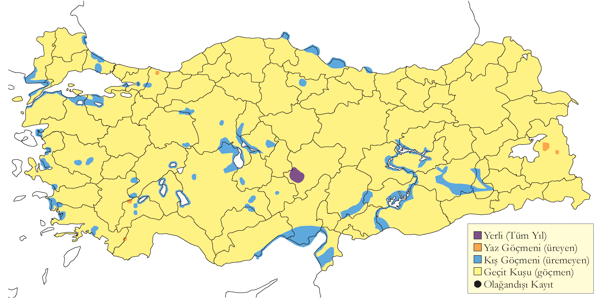
\includegraphics{images/harita_Page_018.png}

\textbf{Üreme}

\textbf{Yuvalama alanı}: Büyük göllerde ve sulakalanlarda yuvalar.\\
\textbf{Yuvası}: Kulu Gölü'ndeki büyük adanın kenarlarındaki
vejetasyonun içinde yuvalamıştır. Yerdeki bir delikte yaptığı yuvasını
bitkisel malzeme, hav tüyü ve biraz tüyle kaplar.\\
\textbf{Yumurta sayısı}: 6-10 yumurta koyduğu kaydedilmiştir.\\
\textbf{Üreme dönemi}: Görünüşe göre mayıs ayında yumurtlar.
\textbf{KAR.} Kızılırmak Deltası'nda üreme davranışları gözlense de
ürediği kesin olarak kanıtlanamamıştır\textsuperscript{44}.
\textbf{AKD.} Hem Haziran 1998 ve Haziran 1999'da Girdev Gölü'nde
yavrular gözlenmiştir. \textbf{İÇA.} 22 Mayıs 1992'de Kulu Gölü'nde yedi
ve on yumurtalı iki yuva, 19 Haziran 1992'de 6 ila 9 yumurtalı beş yuva
bulunmuştur. 24 Haziran 1992'de Bolluk Gölü'ndeki bir çalının altına
gizlenen yuvada 11 yumurta sayılmıştır.

\textbf{Alttürler ve Sınıflandırma}

Türkiye'de nominat alttürü bulunur.

\section{Çıkrıkçın}\label{uxe7ux131krux131kuxe7ux131n}

\emph{Spatula querquedula}, Garganey

\textbf{Yaygın olarak az sayıda üreyen bir yaz göçmenidir. Göç döneminde
daha yaygın ve çok sayıdadır. Nadiren kışlar.}

Ördeklerin arasında esasen yaz göçmen olan tek türdür. Şubat ortasından
itibaren görülmeye başlar, ekim sonuna kadar kalır. Leylekle beraber en
erken gelen yaz göçmenlerindendir. Sazlık sulakalanları tercih eder, en
yoğun ürediği alanlar İç ve Doğu Anadolu'da bulunur. Güneydoğu
Anadolu'da potansiyel olarak iki üreme alanı tanımlanmıştır.

Göçmen sürülerin geçişi şubat sonundan mayıs sonuna kadar devam eder.
Hem ilkbaharda hem de sonbaharda tüm bölgelerde yüzlerce, hatta binlerce
bireylik sürüler halinde görülebilir. Ağustos sonu ve eylül başı
arasında Karadeniz kıyıları boyunca göçmen sürülere rastlanır.

Nadiren Marmara, Ege ve Akdeniz'de az sayıda kışlar. Olağandışı yumuşak
geçen 1968-69 kışında Göksu Deltası'nda 3000 birey ve Gâvur Gölü'nde
5000 birey sayılmıştır. Güncel tarihlerde; Ocak 2002'de Güllük
Deltası'nda 65 birey, Şubat 2002'de Bafa Gölü'nde 58 birey, Aralık
2002'de Çukurova'da 89 birey, 4 Aralık 2010'de Karkamış Barajı'nda iki
birey kışlamıştır.

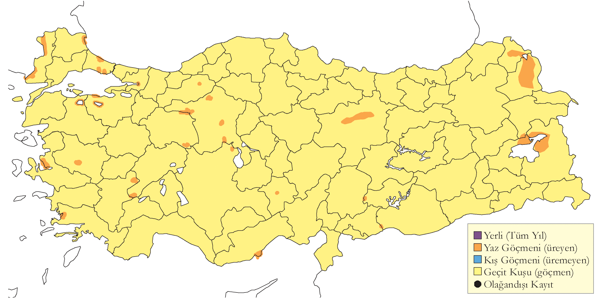
\includegraphics{images/harita_Page_019.png}

\textbf{Üreme}

\textbf{Yuvalama alanı}: Sazlık sulakalanlarda yuvalar.\\
\textbf{Yuvası}: Göl kenarlarındaki ıslak çayırlar, bataklıklar ve
sazlıklarda, ikisinin bir arada olduğu alanlarda ve göl kenarındaki
vejetasyonun içinde ürer.\\
\textbf{Yumurta sayısı}: Türkiye'den veri yoktur, diğer yerlerde olağan
yumurta sayısı 8-11'dir.\\
\textbf{Üreme dönemi}: Nisan ortasından itibaren ürer. Yavrular temmuza
kadar görülebilir. \textbf{KAR.} 19 Mayıs 1992'de Yeniçağa Gölü'nde yeni
bozulmuş ancak yumurtaların taze olduğu açıkça anlaşılan iki yuva, 6
Mayıs 1993'te yakınlardaki ıslak bir çayırlıkta bir yuva bulunmuştur. 13
Mayıs 1986'da Abant Gölü'nde 17 yavru ve bir dişi gözlenmiş, yumurtlama
tarihinin nisan ortası civarında olduğunu hesaplanmıştır. 2 Ağustos
1971'de Kızılırmak Deltası'nda bir çift ve yedi yavru kaydedilmiştir.
\textbf{İÇA.} 10-15 Mayıs 1991'de Hotamış Sazlığı'nda yavrulu birkaç
çift gözlenmiş\textsuperscript{48}, 27 Temmuz 1971'de Kulu Gölü'nde
büyük yavruları olan altı çift kaydedilmiş, Haziran ve Temmuz 1968'de
Mogan Gölü'nde 1-2 kuluçka gözlenmiş, 27 Temmuz 1971'de Yarma'da büyük
yavruları olan en az dört çift tespit edilmiştir.

\textbf{Alttürler ve Sınıflandırma}

Monotipik bir türdür.

\section{Çamurcun}\label{uxe7amurcun}

\emph{Anas crecca}, Eurasian Teal

\textbf{\emph{Lokal olarak az sayıda ürer. Yaygın olarak ve çok sayıda
bulunan kış konuğudur.}}

İç Anadolu, Doğu Anadolu bölgeleri ve Kızılırmak Deltası'nda yuvalar.
Delta'da 1992'de 15-20 çift üremiştir\textsuperscript{44}, Doğu
Anadolu'dan teyit edilmiş üreme kaydı çok azdır.

Geçiş sırasında eylül başından nisan başına kadar ülkenin batı ve orta
bölgelerinde yaygın olarak çok sayıda görülebilir. Marmara ve Karadeniz
bölgelerinde ara sıra yüksek sayılarda kaydedilebilir.

Kışın hem iç bölgelerde hem de kıyısal sulakalanlarda yüksek sayıda
bulunur. Ülke çapında kışlayan nüfus 100.000 birey seviyesindedir. Son
yıllarda kışlayan nüfusta düşüşler yaşanmış, örneğin 1988'de 21.000
birey ve 1989'da 13.400 birey sayılmıştır. Bu düşüş aslında diğer yüzey
ördeklerinde olduğu gibi 60'li yıllardan beri süre gelmektedir.
1968-69'da toplam 270.400 birey ve 1969-70'de 326.700 birey sayılmıştır.
Son sayımda sadece Sultansazlığında 200.000 birey gözlenmiştir. Alanda
sayılan ancak türü tespit edilemeyen 400.000 ördeğin de çamurcun
olabileceği düşünülürse alandaki kışlayan çamurcun sayısı 600.000 birey
olabilir.

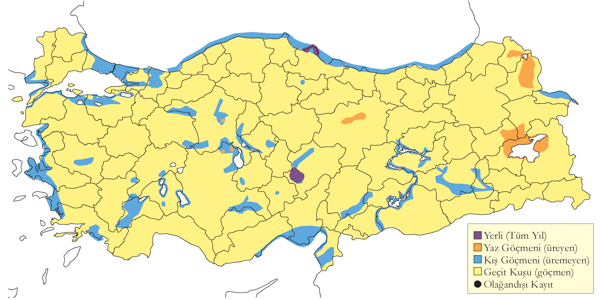
\includegraphics{images/harita_Page_020.png}

\textbf{Üreme}

\textbf{Yuvalama alanı}: Göllerde ve sazlıklarda ürer.\\
\textbf{Yuvası}: Yuva ve yumurta sayısı Türkiye'de tanımlanmamıştır.
Diğer yerlerde yerdeki bir oyuğa yaptığı yuvasını genellikle yapraklar,
bitkisel malzemeler, hav ve kontur tüyleriyle kaplar. Sulakalanlarda
yüksek otların üzerine yuvalar. Nadiren sudan uzağa yuva yapabilir.\\
\textbf{Yumurta sayısı}: Türkiye'den veri yoktur, diğer yerlerde olağan
yumurta sayısı 8-12'dir.\\
\textbf{Üreme dönemi}: Nisan ortasından itibaren ürer. Yavrular temmuza
kadar görülebilir. \textbf{KAR.} 29 Mayıs 1979'da Kızılırmak Deltası'nda
içinde yumurta olan bir yuva bulunmuş, 28 Temmuz 1971'de dokuz yavrulu
bir dişi, 6 Ağustos 1971'de beş yavrulu bir dişi
gözlenmiştir\textsuperscript{24}. 1992'de popülasyonun 15-20 çift olduğu
belirlenmiş, 5 Mayıs'ta dikkati farklı yere çekme davranışı gözlenmiş
ancak hiçbir yuva bulunamamıştır\textsuperscript{44}. \textbf{İÇA.} 14
Mayıs 1991'de Hotamış Sazlığı'nda yavrularıyla birlikte birkaç erişkin
gözlenmiş, buna göre yumurtaların en geç nisan ortasında koyulduğu
hesaplanmıştır\textsuperscript{48}. 5-6 Ağustos 1972'de Kulu Gölü'nde
iki dişinin 7 ve 10 yavrusu gözlenmiştir\textsuperscript{43}.
\textbf{DOA.} 24 Haziran 1983'te Haçlı Gölü'nde tek yavrulu bir dişi
kaydedilmiştir.

\textbf{Alttürler ve Sınıflandırma}

Türkiye'de nominat alttürü bulunur.

\section{Yaz Ördeği}\label{yaz-uxf6rdeux11fi}

\emph{Marmaronetta angustirostris}, Marbled Duck

\textbf{\emph{Türkiye'de üreyen nüfus yok olmuştur.}}

Göksu Deltası'nda üreyen popülasyonun 2013 yılından sonra yokolmasıyla,
üreyen tür olarak soyunun tükendiği söylenebilir. Nadiren Güneydoğu
Anadolu'da görülebilir, Marmara, Ege ve Karadeniz bölgelerinde eski
tarihli kayıtları vardır. En yakın üreme alanı Irak'ta Mezopotamya
Bataklıkları'dır.

Mart başından ekim başına kadar kaydedilen bir yaz konuğu idi. Göksu
Deltası'nda üreyen popülasyon 1989 ile 2013 arasındaki adım adım
azalmıştır. 1989 ve 1991'de yaklaşık 50 çift tespit edilmiş, 2000'li
yıllarda 10 çifte düşmüş, 2010 ve 2013 arasında sadece 1 ila 2 çift
kalmış, 2014 yılından itibaren alanda görülmemeye başlamıştır. Bu
nedenle Türkiye'de üreyen nüfusunun yok olduğu kabul
edilmiş\textsuperscript{46} ve Yaz Ördeği Yılanboyun'dan sonra
Türkiye'de soyu tükendiği belgelenen kuş ilk türü olmuştur.

1987 yılında Çukurova'da bugün yok edilmiş olan Dipsiz Gölü'nde 32 çift
tespit edilmiştir. İç Anadolu'da Ereğli Sazlığı'nda muhtemelen 1-4 çift,
Hotamış Sazlığı'nda 10-15 çift, Sultansazlığı 1-4 çift üremiştir. Van
Gölü havzasında; Erciş Gölü ve Van Sazlığı'nda az sayıda ürediği teyit
edilmiş, bunun yanında Ağrı çevresi, Ahlat Sazlıkları, Bendimahi Deltası
ve Kuyucuk Gölü'nde üreme döneminde görülmüştür. 1987 yılında ülke
nüfusunun da 50-100 çiftin olduğu düşünülmüştür. Üreme sonrasında
Çukurova ve Göksu Deltasında 100-200 bireyin toplandığı bilinir. Nadiren
az sayıda kışlamıştır. En son sayımlarda 1993'te Çukurova'da dört,
1997'de aynı alanda 35 birey sayılmıştır.

Amik Gölü'nün kurutulmasında önce muhtemelen önemli sayılarda
bulunuyordu\textsuperscript{49}. Konya havzasında bulunan Yarma
Sazlıkları, Gönenç Gölü ve Karapınar Ovası'nda\textsuperscript{50}
muhtemelen üremiştir. Mogan Gölü ve Eber Gölü gibi diğer birkaç alanda
da muhtemelen üremiştir. Bu alanlar ekolojik özelliklerini kaybettikleri
ve türe uygun üreme habitatları barındırmadıkları için artık üremeye
elverişli değildirler. Üreme sonrası toplanan bireyler o yıllarda toplam
ülke nüfusu konusunda fikir verebilir. Ağustos 1967'de Çukurova'da 2000
birey ve Göksu Deltası'nda 450 birey sayılmıştır.

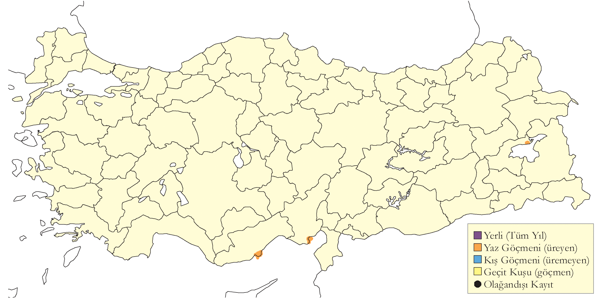
\includegraphics{images/harita_Page_021.png}

\textbf{Üreme}

\textbf{Yuvalama alanı}: Çukurova ve Göksu Deltası'nda sığ ve ötrofik
göllerde bulunmuştur. Genellikle sazlık adaların, bitişik havuzlar ve
sazlıkların bulunduğu yoğun sualtı vejetasyonuna sahip sığ göllerin
çevresinde ürer ve geniş sulakalanları tercih eder. Sanılanın aksine acı
veya tuzlu sularda değil, tatlı suları tercih eder.\\
\textbf{Yuvası}: 9 Haziran 1993'te Göksu'da, kofanın (\emph{Juncus})
baskın olduğu ve yakınlarda sazların (\emph{Phragmites}) da bulunduğu
bataklık bölgede sığ gölcüklerin olduğu bir alanda, yaklaşık 1 m.
çapındaki bir \emph{Juncus} kümesinin içinde, sudan yaklaşık 0,7 m
yüksekte iyice gizlenmiş bir şekilde yumurtaların henüz tamamlanmadığı
iki yumurtalı bir yuva bulunmuştur. Çok daha fazla yumurta için
yapıldığı açıkça belli olan, sazlardan ve bitki gövdelerinden yapılmış
dayanıklı ve derin bir kâse şeklindeki yuva daha ince bitkisel
malzemeyle kaplanmış, hiç hav tüyü kullanılmamıştır.\\
\textbf{Yumurta sayısı}: 2-12 arasında değişir, ortalama yumurta sayısı
6,5 olarak hesaplanmıştır\textsuperscript{51}. Başka yerlerdeki tipik
yumurta sayısı 9-13'tür (5-18).\\
\textbf{Üreme dönemi}: 22 Mayıs 1971'de Çukurova'da kaydedilen altı
yavru en erken kayıttır ve yumurtlamanın nisanın ikinci yarısında
başladığını gösterir. Ana yumurtlama dönemi mayısın ikinci yarısıyla
haziran başı arasındadır. Yavrular en erken 7 Haziran'da ortaya çıkarlar
ve temmuz sonuna kadar küçük yavrular görülebilir. Tamamen palazlanmış
yavrular temmuz başında kaydedilmiştir. \textbf{AKD.} 1991'de Göksu
Deltası'nda yaklaşık 50 çiftin en az 31'İ yavru çıkarabilmiştir. 1991'de
Göksu Deltasında 11 yuvada 8-13 yavru, 5 yuvada 4-6 yavru ve bir yuvada
15 yavru sayılmıştır. 15 yavrunun iki dişinin yumurtalarının bir araya
gelerek oluşturmuştur. Benzer şekilde 15-18 Temmuz 1992'de bir dişi 32
yavruyla görülmüştür\textsuperscript{51}. 10 Temmuz 1967'de kaydedilen
hem büyük hem de küçük yavrular az sayıda haziran ve daha çok temmuzda
gözlenmiştir\textsuperscript{52}. \textbf{İÇA.} 4-5 Haziran 1971'de
Yarma Sazlığı'nda 6 ve 13 yumurtalı iki yuva bulunmuş, bir yuvada bir
Yeşilbaş yumurtasına rastlanmıştır. 12 Haziran 1998'de Kulu Gölü'nde tek
yavrulu bir erişkin kaydedilmiş ve temmuzda üç farklı alanda yavrular
gözlenmiştir. \textbf{DOA.} 22 Temmuz 1987'de Van Sazlığı'nda küçük
yavruları olan iki çift gözlenmiş, bu gözleme göre yumurtlamanın haziran
ortasında olduğunu tahmin edilmiştir. Aynı alanda temmuz sonunda ve
ağustos başında genç bireyler kaydedilmiştir.

\textbf{Alttürler ve Sınıflandırma}

Monotipik bir türdür.

\section{Macar Ördeği}\label{macar-uxf6rdeux11fi}

Netta rufina, Red-crested Pochard

\textbf{\emph{Lokal olarak nispeten çok sayıda ürer. Kışın daha
yaygındır ve bazı alanlarda yüksek sayılarda toplanır.}}

İç Anadolu'daki geniş sodalı ya da tatlı sazlık sulakalanlarda çok
sayıda ürer. Sultansazlığı'nda yüksek sayıda bulunur. 1990'larıda Ereğli
Sazlığı'nda 500 çift, 1998'de sadece 20 çift üremiş, sonra alanın
kurutulmasıyla alandan yok olmuştur. Kızılırmak Deltası'nda 1992'de
50-75 çift üremiştir\textsuperscript{44}. Diğer alanlarda nispeten
yüksek sayılarda yuvalayanlar yerli veya yarı göçmendir. Çukurova
sulakalanları ve Göksu Deltası'nda üreyen nüfus 1990'dan sonra
azalmıştır. Türkiye'de üreyen popülasyon 1000-5000 çift olarak tahmin
edilmiştir\textsuperscript{41}. Son yıllarda İç Anadolu'da üreyen
kuşların sayılarında yaşanan azalma, güncel ulusal nüfusun çok daha az
olduğuna işaret eder. \footnote{Kerem Okudu 15 Haziran}

Ülke genelinde geçiş sırasında doğu bölgeleri dışında daha yaygındır.
Çoğu zaman yüzeyi donmaya daha az eğilimli olan baraj göllerini tercih
eder. Ocak 1967'de 12.000 birey sayılmış olup, bunun 7000 tanesi bugün
kurutulmuş Amik Gölü'ndendir. Türkiye genelinde 1992'de 5249, 1996'da
6522 ve 1999'da 6228 birey sayılmıştır. 2000'lı yıllarda toplam sayıda
artma görülmüş, sadece Beyşehir Gölü'nde Şubat 2003'te 10.000 birey ve
Ocak 2005'te 20.000 birey sayılmış, son sayımda hem toplam hem de alan
rekoru kırılmıştır.

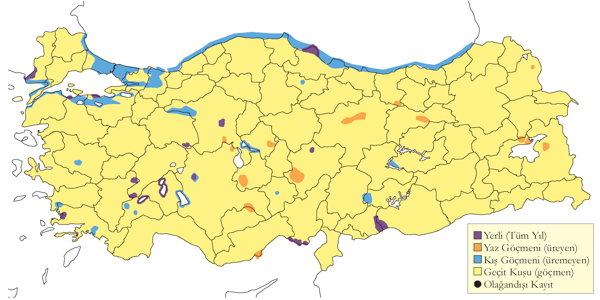
\includegraphics{images/harita_Page_022.png}

\textbf{Üreme}

\textbf{Yuvalama alanı}: Yoğun sazlıkların ve su kenarı bitkilerinin
bulunduğu tatlı ya da sodalı göllerde ve su aynalarına sahip sazlıklarda
ürer.\\
\textbf{Yuvası}: Yerdeki bir oyuğa yaptığı yuvasını bitkisel malzeme,
hav tüyleri ve tüylerle kaplar. Çoğunlukla yoğun vejetasyonun içine,
nadiren açıkta (örneğin adalarda) ya da nemli alanlarda su seviyesinin
üzerindeki saz öbeklerinin ya da diğer sucul bitkilerin içine genellikle
iyice gizlenmiş bir yuva yapar.\\
\textbf{Yumurta sayısı}: Türkiye'de gözlenen yumurta sayısı 4-12 olup,
ortalama 8,3'tür (18 yuvada). Bir yuvada bulunan 24 yumurta muhtemelen
birden fazla dişiye aittir. Yavru sayısı 2-12 arasında değişir, 16
yuvada ortalama 6,2'dir. Sadece 2-4 yavru çıkarabilmiş 6 dişi ortalamayı
düşürmüştür.\\
\textbf{Üreme dönemi}: Nisan sonu ile temmuz başı arasında yumurtlar.
Yavrular temmuz sonuna kadar görülebilir. \textbf{MAR.} 1 Mayıs 1993'te
Kocaçay Deltası'nda yumurtalı bir yuva bulunmuştur\textsuperscript{45}.
\textbf{KAR.} Kızılırmak Deltası'nda 27 Mayıs 1992'de beş yumurtalı bir
yuva bulunmuş, 4 Haziran 1992'de yaklaşık bir haftalık ilk tüylü yavru
kaydedilmiş\textsuperscript{44} ve 27 Mayıs 1979'da sekiz yavrulu bir
aile gözlenmiştir\textsuperscript{24}. \textbf{AKD.} 18 Temmuz 1992'de
Karamık Gölü'nde küçük yavrulardan oluşan bir aile gözlenmiştir.
\textbf{İÇA.} Çoğu mayısta olmak üzere 25 Nisan'da yumurta kayıtları
vardır. En geç kayıt 19 Haziran 1992'de 12 yumurtalı bir yuvadır. Biri
11 Mayıs'ta, çoğu haziranda olan birçok yavru kaydı vardır, en geç 8
Temmuz 1967'de\textsuperscript{52} ve 5 Ağustos 1972'de küçük yavrular
gözlenmiştir. \textbf{DOA.} 21-22 Temmuz 1986'da Van Gölü'nde 7-8
yavrulu üç yavrulu bir aile kaydedilmiştir.

\textbf{Alttürler ve Sınıflandırma}

Monotipik bir türdür.

\section{Elmabaş Patka}\label{elmabaux15f-patka}

\emph{Aythya ferina}, Common Pochard

\textbf{Nispeten yaygın ve çok sayıda bulunan yerli ve yarı göçmen,
yaygın ve çok sayıda bulunan kış konuğudur.}

İç ve Doğu Anadolu'daki sulakalanlarda orta sayılarda üreyen yerli ve
yarı göçmendir. 1992'de Kızılırmak Deltası'nda 300-350 çiftin ürediği
tahmin edilmiştir\textsuperscript{44}. Uygun habitatların azlığı
nedeniyle Karadeniz, Güneydoğu Anadolu ve belki de diğer bölgelerde
lokaldir. Muhtemelen gerçek üreme durumunu çarpıtacak şekilde hatırı
sayılır sayıda üremeyen birey özellikle İç ve Doğu Anadolu'da yazı
geçirir.

Kışın ve geçiş sırasında ülke genelinde yaygın ve boldur. Son yıllarda
ortalama 67.000 bireyden fazla sayılmaktadır. 1996 yılında Beyşehir
Gölü'nde 47.000, Uluabat Gölü'nde 42.000 ve ülke toplamında sayılan
250.000 birey en yüksek sayımlardır. 1999'da Eğirdir Gölü'nde 40.000,
ülke toplamında 137.000 kuş sayılmıştır. 18 yıllık Kış Ortası Su kuşu
sayımlarının ortalaması 93.000 kuştur. İstisna olarak 1968-69 kışında
355.000 bireyin kışladığı tahmin edilmiştir. Ekim ortasından itibaren
yüksek sayılar gelir; Göksu Deltası'nda Ekim 1978'de 40.000, Ekim
2002'de Sodalıgöl'de 100-130.000, Kulu Gölü'nde Kasım 1970'de 45.000, ve
Kasım 1971'de 28.000 birey kaydedilmiştir.

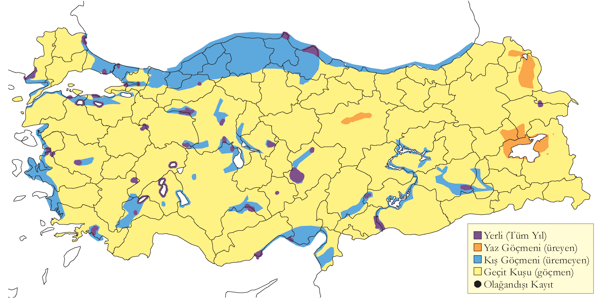
\includegraphics{images/harita_Page_023.png}

\textbf{Üreme}

\textbf{Yuvalama alanı}: Sazlıkların olduğu göllerde ve su aynalarının
bulunduğu geniş sazlıklarda ürer.\\
\textbf{Yuvası}: 19 Haziran 1984'te Erçek Gölü yakınlarındaki küçük bir
gölde sık bir örtü içindeki sazların dibine tutturulmuş sakarmeke
yuvasına benzer şekilde sudan yükseğe yapılmış bir yuva bulunmuştur; ölü
saz gövdeleri ve diğer bitkisel malzemelerin derin, düzgün bir kâse
şeklinde iç içe örülmesi ile oluşmuş dayanıklı bir yapı olan yuva bol
miktarda hav tüyü ve biraz da diğer tüylerle kaplanmıştır. Diğer
yerlerde, yuvalar genellikle benzer alanlardadır, nadiren su kıyısındaki
yoğun bitki örtüsünün içinde kuru zeminde de olabilir.\\
\textbf{Yumurta sayısı}: Türkiye'de yumurta sayısı kaydedilmemiştir,
gözlenen yavru sayısından 8-11 yumurta koyabileceği düşünülür. Diğer
yerlerde genellikle 6-9 yumurtadır. Gözlenen yavru sayısı ortalama
6,6'dır.\\
\textbf{Üreme dönemi}: Nisan başı ile haziran ortasına kadar yumurta
koyar. Yavrular temmuzda gözlenebilir. \textbf{KAR.} Kızılırmak
Deltası'nda, 11 Mayıs 1992'de hav tüyleriyle gözlenen birkaç günlük
yavru en erken kayıt\textsuperscript{44} yumurtlamanın nisanın ilk
haftasında olduğunu gösterir. 14 Haziran 1984'te yaklaşık 5 günlük bir
yavrulardan oluşan bir kuluçka ve yaklaşık üç haftalık yavrulardan
oluşan iki kuluçka gözlenmiştir\textsuperscript{24}. \textbf{İÇA.}
Haziran başlarında iki yumurtalı (tamamlanmamış) bir yuva bulunmuş ve
Haziran 1971 başlarında boz ördek yuvalarına iki, dört ve beş yumurta
bıraktığı tespit edilmiştir; 13 Mayıs 1991'de Hotamış'ta yumurtalı bir
yuva bulunmuştur\textsuperscript{48}. 1970 Mayıs sonlarında Eşmekaya'da
küçük yavrulardan oluşan beş yavru, 1 Haziran 1969'da Sultansazlığı'nda
altı yavru ve haziran-temmuzda diğer alanlarda da yavrular gözlenmiştir.
\textbf{DOA.} 19 Haziran 1983'te Van Sazlığı'nda yavrularıyla birlikte
sekiz dişi kaydedilmiştir.

\textbf{Alttürler ve Sınıflandırma}

Monotipik bir türdür.

\section{Pasbaş Patka}\label{pasbaux15f-patka}

Aythya nyroca

Ferruginous Duck

\textbf{Lokal olarak az sayıda üreyen yaz konuğu, yaygın ve nispeten çok
sayıda bulunan geçit türü, yaygın ancak az sayıda kış konuğudur.}

Tüm bölgelerdeki sulakalanlarda oldukça lokal bir yaz konuğudur. En
yüksek sayılarda İç ve Doğu Anadolu bölgelerinde bulunur. Kızılırmak
Deltası (1992'de tahminen 150-200 çift\textsuperscript{44}), Kocaçay
Deltası (1993'te tahminen 70 çift\textsuperscript{45}), Uluabat Gölü
(1988'de tahminen 32 çift\textsuperscript{53}) ve Göksu Deltası
(yaklaşık 30 çift) önemli sayılarda ürediği alanlardır. Son yıllarda
gerçekleştirilen çalışmalarda Güneydoğu Anadolu'da üç yeni üreme alanı
belirlenmiştir. Yaz göçmenleri mart ortasından eylül sonuna kadar
gözlenir.

Türkiye popülasyonu muhtemelen dünyadaki en önemlilerinden biridir ve
1000 ile 3000 çift arasında olduğunu düşünülmüş\textsuperscript{41},
sonra bu tahmin 500-600 çift olarak güncellenmiştir\textsuperscript{54}.
Avrupa'da yayılış alanının bir kısmında yaşanan sert düşüş dikkate
alındığında, Türkiye popülasyonun izlenmesine acil ihtiyaç
duyulmaktadır. 1990'ların sonlarında İç Anadolu'daki birkaç alanda da
azalma görülmüştür.

Geçiş sırasında az ve orta sayılarda bulunur ve ülke genelinde biraz
daha yaygındır. Az sayıda kışlar, 1992 yılında 105 birey, diğer yıllarda
50 bireyden az sayılmıştır. 1990'ların ortalarından itibaren kış
kayıtlarında bir artış gözlenmiş, bu durum muhtemelen gözlemci sayısının
artmasına bağlanmıştır. Eskiden batı ve orta bölgelerde daha çok sayıda
kışlamış, 1968-74 yıllarında 50 ile 450 birey arasında kaydedilmiştir.
Marmara Gölü'nde kaydedilen 860 birey en yüksek kayıttır. Doğu ve
Güneydoğu Anadolu'daki 2005 yılında sayılan 44 birey bahsedilmeye
değerdir.

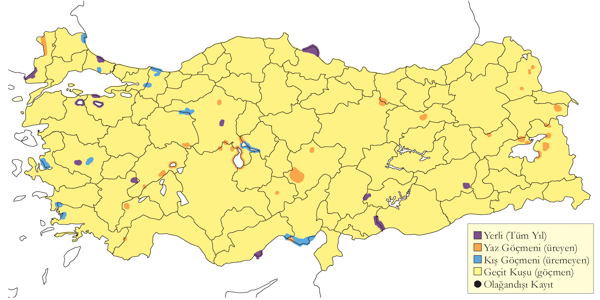
\includegraphics{images/harita_Page_024.png}

\textbf{Üreme}

\textbf{Yuvalama alanı}: Çevresinde sazlıkların ve yoğun su üstü
vejetasyonunun ve çoğunlukla daha geniş sazlıkların ve bataklığın
bulunduğu tatlı su göllerinde ürer.\\
\textbf{Yuvası}: Su kenarındaki yoğun vejetasyonun içine yuva yapar:
Kulu Gölü'ndeki bir adada, alçak çalıların arasında çıplak zeminde hafif
bir çukurun içine yapılan yuvanın ot ve hav tüyleriyle kaplandığı
gözlenmiştir (\textsuperscript{55}; A. Limbrunner, kişisel görüşme).\\
\textbf{Yumurta sayısı}: Türkiye'de gözlenen yumurta sayısı 6-8
arasındadır.\\
\textbf{Üreme dönemi}: Nisan ile Haziran başı arasında yumurta koyar.
Yavrular ağustosa kadar gözlenebilir. \textbf{MAR.} 19 Haziran 1999'da
Uluabat Gölü'nde bazıları küçük yavrulardan oluşan birkaç yavru grubu
gözlenmiş, 1966'da Manyas Gölü'nde yavru kaydedilmiştir. \textbf{KAR.}
Kızılırmak Deltası'nda çiftlerin çoğu sazlık alanlarda gözlenmiştir; 5
Mayıs 1992'de altı yumurtalı bir yuva bulunmuş ve 1 Haziran 1992'de
yumurtlamanın nisan sonlarından daha geç olmadığını gösteren üç ve dört
yavrulu iki grup\textsuperscript{44} kaydedilmiştir. 6 Ağustos 1971'de
yedi yavrulu bir grup gözlenmiştir. \textbf{AKD.} 15 Mayıs 1962'de
Çukurova'da sekiz yumurtalı bir yuva\textsuperscript{54}; 8 Mayıs
1953'te Amik Gölü'nde yumurtalı bir yuva\textsuperscript{54}; ve 27
Mayıs 1933'te yumurta kanalında yumurta bulunan bir dişi
vurulmuştur\textsuperscript{56}; Göksu Deltası'nda en erken 17
Haziran'da olmak üzere yedi savunma alanında yavrular gözlenmiştir.
\textbf{İÇA.} 28 Nisan 1982'de Sultansazlığı'nda yumurtalı bir yuva
bulunmuştur\textsuperscript{54}, Mayıs 1973'te Kulu Gölü'nde altı
yumurtalı bir yuva bulunmuştur; en erken 20 Haziran'da Eber Gölü'nde
olmak üzere Çöl Gölü, Gönenç Gölü, Sultansazlığı, Mogan Gölü ve Kulu
Gölü'nde yavrular gözlenmiştir. \textbf{DOA.} Yumurtlamanın mayıs
sonunda olduğunu gösterecek şekilde 1985 ve 1987 Haziran sonunda Van
Gölü'nde ve 29 Haziran 1987'de Edremit Sazlığı'nda yavrular
gözlenmiştir\textsuperscript{54}.

\textbf{Alttürler ve Sınıflandırma}

Monotipik bir türdür.

\section{Tepeli Patka}\label{tepeli-patka}

\emph{Aythya fuligula}, Tufted Duck

\textbf{\emph{Lokal ve az sayıda üreyen yaz konuğu, nispeten yaygın ve
çok sayıda bulunan kış konuğudur.}}

Çok nadir ve lokal olarak üremiştir. Kızılırmak Deltası'nda, 1967 ve
1981'de Çalı Gölü'nde (Kars) ürediği kanıtlanmış ve son alanda 20
çiftlik bir popülasyon tespit edilmiştir. Başka bölgelerde düzenli
olarak yazı geçirir. Uluabat Gölü ve Uyuz Gölü gibi bazı alanlardaki
uygun habitatlarda çiftler gözlenmiştir. Üreme sonrasında Temmuz 1982'de
Kulu Gölü'nde tüy değişimi için toplandıkları düşünülen 700
birey\textsuperscript{43}, Eylül 1967'de Sodalı Gölü'nde çoğu erkek olan
1200 birey sayılmıştır.

Ülkenin batı ve orta bölgelerinde eylül başından nisanın başına kadar
kaydedilen yaygın ve bol olan bir geçiş türü ve kış konuğudur.
Karadeniz'de denizde kışlar. Kış ortası sayımlarında; 1968-69 kışında
20.800 birey, 1996 yılında en yüksek sayı olan 58.271 birey, 1992'de
yaklaşık 13.000 birey, 1993'te 16.965 birey (sadece Eğirdir Gölü'nde
10.478 birey) ve 1999'da 18.512 birey kaydedilmiştir. Son yıllarda ise
ülke toplamı genellikle 5000-10.000 birey arasındadır. En önemli kışlama
alanı Sapanca Gölü ve Eğirdir Gölü'dür.

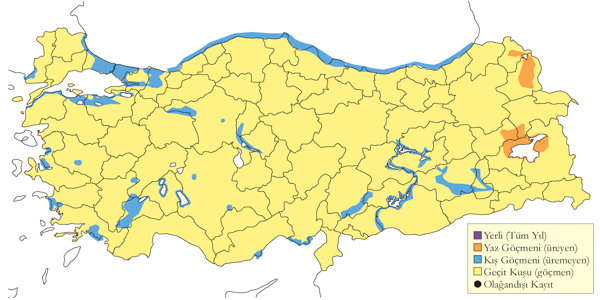
\includegraphics{images/harita_Page_025.png}

\textbf{Üreme}

\textbf{Yuvalama alanı}: Su üstü vejetasyonuna sahip olan tatlı su
göllerinde ürer.\\
\textbf{Yuvası}: Yuvasını bir bitki öbeğinin altına kurar.\\
\textbf{Yumurta sayısı}: Türkiye'de 8 yumurtalı bir yuva bulunmuştur.\\
\textbf{Üreme dönemi}: Mayıs ayında yumurta koyar, temmuz sonuna kadar
yavrular görülebilir. \textbf{KAR.} Kızılırmak Deltası'nda, 5 Mayıs
1992'de sazlıkta bir \emph{Juncus acutus} öbeğinin dibinde sekiz
yumurtalı bir yuva bulunmuş\textsuperscript{44} ve 28 Mayıs 1968'de de
ürediği kanıtlanmıştır\textsuperscript{24}. \textbf{DOA.} Çalı Gölü'nde
19 Temmuz 1992'de yavrularıyla birlikte iki dişi
gözlenmiştir\textsuperscript{57}.

\textbf{Alttürler ve Sınıflandırma}

Monotipik bir türdür.

\section{Karabaş Patka}\label{karabaux15f-patka}

\emph{Aythya marila}, Greater Scaup

\textbf{\emph{Özellikle Karadeniz kıyılarında az sayıda ve düzenli
olarak görülen kış konuğudur.}}

Karadeniz ve Marmara Bölgesi'nde hemen hemen her yıl az sayılarda
görülmektedir. Modern kuş tayinin başlaması sonrasında gelen kayıtlar
şöyledir\textsuperscript{1--4}: Ocak-Şubat 1969'da Sakarya Deltası'nda
yedi birey, Manyas ya da Uluabat Gölü'nde dört birey görülmüştür.
Kızılırmak Deltası'ndaki Liman Gölü'nde 1990'ların başlarında kışlayan
38 birey, 1970'lerde aynı alandan bildirilen şüpheli
kayıtların\textsuperscript{24}geçerli olabileceğini düşündürür.

Çoğu İstanbul civarından olan geçmiş veriler şöyledir: Şubat 1893'te,
Çekmece'de daha çok dişi ve gençlerden oluşan bir grup gözlemiş ve şu
anda Sofya Doğa Tarihi Müzesi'nde bulunan erkek örnek
toplanmıştır\textsuperscript{58}. İstanbul Robert Kolej'de bulunan dişi
örnek\textsuperscript{21}, 1998'deki bir ziyarette
bulunamamıştır\textsuperscript{59}. 1946-47 ve 1947-48 kışlarında
Çatalağzı açıklarında (Zonguldak) belirsiz sayıda
gözlenmiş\textsuperscript{60}, 15 Ocak 1950'de bilinmeyen bir yerden
altı örnek alınmıştır\textsuperscript{18}. Büyükçekmece'de Ocak 1963'te
bir erkek ve Şubat 1964'te bir dişi kaydedilmiştir\textsuperscript{18}.

Türün ilk yaz kaydı 30 Mayıs 1992'de Sodalı Gölü'nde kaydedilen iki
erkektir\textsuperscript{9}. Öte yandan, 19 Nisan 1981'de Kulu Gölü'nde
gözlenen iki birey, 12 Nisan 1990'da Göksu Deltası'nda gözlenen yaklaşık
20 birey\textsuperscript{10} olağandışı geç kayıtlardır.

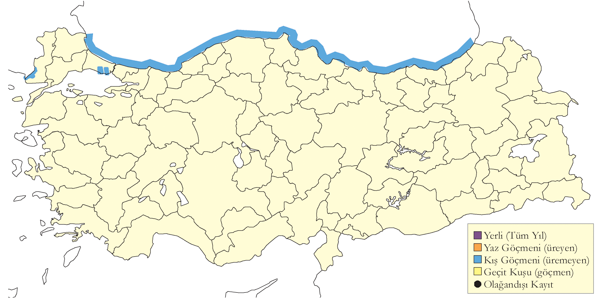
\includegraphics{images/harita_Page_026.png}

\textbf{Üreme}

Türkiye'de yuvalamaz. Avrasya ve Kuzey Amerika'nın kuzeyinde yuvalar.

\textbf{Alttürler ve Sınıflandırma}

Türkiye'de nominat alttürü bulunur.

\section{Pufla}\label{pufla}

\emph{Somateria mollissima}, Common Eider

\textbf{\emph{Karadeniz kıyılarında nadiren az sayıda görülür.}}

İlk üç kayıt şu şekildedir: 20 Eylül 1983'te Çernek Gölü'nde (Kızılırmak
Deltası) bir erkek\textsuperscript{24}, 3 Ocak 1984'te Göksu Deltası'nda
ölü bir dişi\textsuperscript{61}, 1 Şubat 1997'de, Sakarya Nehri
deltasının batısında Kefken açıklarında iyi tanımlanmış ilk kışında bir
erkek ve iki dişi\textsuperscript{62}bulunmuştur. Bundan sonra Riva,
Terkos Gölü kıyıları, İğneada, Kızılırmak Deltası, İzmit Körfezi ve
Sakarya Karasu'da 20'den fazla kayıtta 1-3 birey tespit edilmiştir.

Türkiye'de üremez, en yakın üreme kolonisi Ukrayna kıyılarındadır.
Güvenilir kayıtların tümü 1975 yılında Ukrayna'nın Karadeniz kıyısında
bir üreme alanının keşfedilmesinden sonra olmuştur. Bu popülasyon
1990'ların ortasına kadar 1000 çifte ulaşmıştır ve günümüze kadar
artmaya devam etmektedir.

Şubat 1929'un ilk yarısında Tarabya ile Beykoz arasında (İstanbul
Boğazı) gözlenen bir erişkin erkek\textsuperscript{18} tanım olmadığı
için burada kabul edilmemiştir.

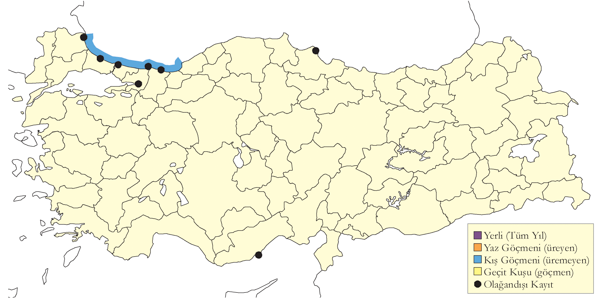
\includegraphics{images/harita_Page_027.png}

\textbf{Üreme}

Türkiye'de yuvalamaz. Ukrayna'daki koloni insan eli ile geliştirilmiş ve
bugün doğallaşmıştır. Doğal yuvalama alanı Kuzey Atlantik, Kuzey Buz
Denizi ve Bering Boğazı'dır.

\textbf{Alttürler ve Sınıflandırma}

Ülkede gözlenen ırk nominat \emph{mollissima} (Kuzeybatı Avrupa)
alttürüdür.

\section{Kadife Ördek}\label{kadife-uxf6rdek}

\emph{Melanitta fusca}, Velvet Scoter

\textbf{\emph{Türkiye'de üreyen nüfus yok olmuştur. Karadeniz kıyılarına
az sayıda kışlar.}}

Doğu Anadolu'da az sayılarda kaydedilen çok lokal bir yaz konuğu idi. Az
sayıda yüksek irtifa göllerinde 3000 m'nin üstünde üremiş olduğu
düşünülür. Aktaş Gölü (Ardahan) kesin olarak ürediği tek alandır. 3 Ekim
1980'de 100 birey\textsuperscript{63} ve 14-15 Temmuz 1994'te aralarında
gençlerin de bulunduğu 725 birey\textsuperscript{64} kaydedilmiştir.

Geçmişte Nemrut Dağı'ndaki (Tatvan) krater Gölü'nde 20 çifte ürediği
düşünülmüştür. Ağrı Balık Gölü geçmişte ürediği sanılmış, ancak görünüşe
göre Haziran 2001'de (artık) üremediğine karar kılınmıştır. Çıldır
Gölü'nde ürediği güçlü şekilde şüphelenilmiş, ancak teyit edilmemiştir.
Kars Aygır Gölü ve Muş Nazik Gölü'nde azami 32 birey yazı geçirmiştir.
Doğu Karadeniz kıyılarında kışlayan bireylerin yaz aylarında da kaldığı
gözlenmiştir.

Gürcistan'da yuvalamaya devam eden bireyler, Karadeniz kıyılarına az
sayıda kışlar. Orta ve Doğu Karadeniz boyunca az sayıda kışlar. 1995
Aralık sonunda Yeşilırmak Deltası'nda 870 birey en yüksek kayıttır.
Nadir olarak Batı Karadeniz, Marmara'da ve güneyde Akdeniz kıyısında
kışlamıştır. Ocak 1970'de Burdur Gölü'nde 27 birey, Şubat 1966'da Mogan
Gölü'nde ve Ocak 2005'te Hazar Gölü'nde kaydedilmiştir. Son yıllarda
kaydedilen 50 birey

4 Şubat 1917'de İstanbul Zeytinburnu açıklarında gözlenen iki birey ülke
için ilk kayıttır.

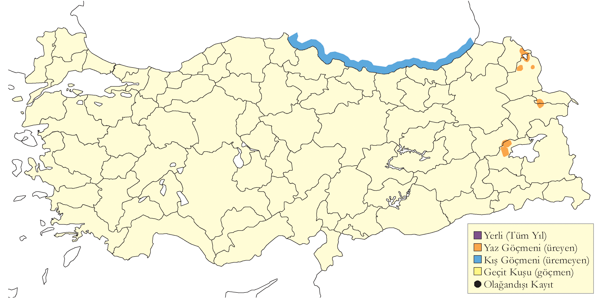
\includegraphics{images/harita_Page_028.png}

\textbf{Üreme}

\textbf{Yuvalama alanı}: Doğu Anadolu'daki iki ya da üç yüksek irtifa
gölünde üremiştir. Tüm çabalara rağmen Türkiye'de yuvası bulunamamıştır.
Şu anda Kafkasya popülasyonu sadece Gürcistan'da bir gölde
yuvalamaktadır.\\
\textbf{Yuvası}: Türkiye'de yuva bulunmamıştır ancak diğer yerlerde
yoğun bitki örtüsünün içine gizlenmiş şekilde yerde ve genellikle
göllerdeki adalarda yuva yapar.\\
\textbf{Yumurta sayısı}: Olağan yumurta sayısı 7-10'dur.\\
\textbf{Üreme dönemi}: Eski gözlemlere göre temmuz ve ağustos ayında
yuvalamıştır. \textbf{DOA.} 10 Temmuz 1967'de Nemrut Dağı'ndaki krater
Gölü'nde iki, yedi ve dokuz hav tüylü küçük yavru birlikte üç dişi ve 20
Ağustos 1967'de Balık Gölü'nde dört, beş ve altı yavrulu üç dişi
kaydedilmiştir\textsuperscript{52}. Küçük ördeklerin sadece yaklaşık bir
haftalık olduğu varsayılırsa yumurtlamanın haziranın ilk günlerinde
olduğu anlaşılmaktadır. 23 Ağustos 1972'de Nemrut Dağı'nda gözlenen
hemen hemen yarı gelişmiş yedi yavrulu bir dişi yumurtlamanın haziranın
son haftası olduğunu göstermektedir. 9 Temmuz 1985'te Nemrut Dağı'nda
beş çift ve iki genç birey gözlenmiştir. Son zamanlara ait bir üreme
kaydı yoktur ve 9 Haziran 2001'de Balık Gölü'ndeki adada yapılan
kapsamlı araştırmada ne yuva bulunmuş ne de erişkin görülmüştür.

\textbf{Alttürler ve Sınıflandırma}

Monotipik bir türdür. Eskiden Amerika ve Doğu Sibirya'da yaşayan
\textbf{Ak Kanatlı Kadife Ördek} \emph{Melanitta deglandi} ile aynı tür
olarak kabul ediliyordu.

\section{Kara Ördek}\label{kara-uxf6rdek}

\emph{Melanitta nigra,} Common Scoter

\textbf{\emph{Nadir kış konuğudur.}}

Karadeniz'de çoğunlukla eylül ve mart arasında çok az sayıda kaydedilen
kış göçmenidir. Düzenli olarak sadece Kızılırmak ve Yeşilırmak
Deltalarının açıklarında 20 birey kışlamaktadır. Karadeniz kıyısında
toplam 20'den fazla kaydı vardır. Marmara ve Ege'de çok nadirdir,
Akdeniz'de sadece bir kere kaydedilmiştir.

9 Nisan 1967'de Kocaçay Deltası'nda kaydedilen bir birey ülke için kabul
edilebilir ilk kayıttır\textsuperscript{1}. Öncesinde Ege'de nadir bir
kış göçmeni olduğunundan\textsuperscript{65} ve İstanbul Boğazı ve
Ceyhan Deltası'ndaki şüpheli kayıtlardan\textsuperscript{28}
bahsedilmiştir.

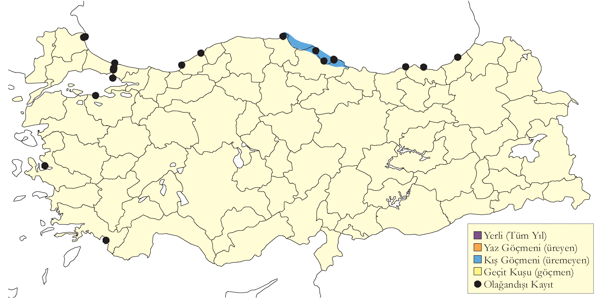
\includegraphics{images/harita_Page_029.png}

\textbf{Üreme}

Türkiye'de yuvalamaz. Avrasya'nın kuzeyinde yuvalar.

\textbf{Alttürler ve Sınıflandırma}

Monotipik bir türdür.

\section{Telkuyruk}\label{telkuyruk}

\emph{Clangula hyemalis}, Long-tailed Duck

\textbf{\emph{Nadir kış konuğudur.}}

Şubat 1893'te İstanbul (Büyük?) Çekmece'de, Alléon tarafından toplanan
genç bir dişi ülke için ilk kayıttır ve bu örnek Sofya Doğa Tarihi
Müzesi'nde görülebilir. Ardından, 13 Kasım 1968'de İzmit'te genç bir
birey kaydedilmiştir\textsuperscript{3}. Göksu Deltası Paradeniz
Gölü'nde 1-2 Ocak 1986'da bir birey ve 5 Ocak 1989'da bir
dişi\textsuperscript{61} görülmüştür. Sakarya Nehri ağzında 18 Şubat
2004'te\textsuperscript{66}; 26 Şubat 2006'da Fırtına Nehri'nin ağzında
birer birey fotoğraflanmıştır. En güncel kayıtlara göre; 7-19 Ocak
2008'de İğneada'da erişkin bir dişi, 13 Şubat 2008'de Kıyıköy'de bir
erkek, 10 Aralık 2008'de İğneada'da bir birey (onüçüncü kaydı) ve 28
Mart 2009'da Enez'de bir birey (on dördüncü kaydı)
görülmüştür\textsuperscript{8}.

İstisnai olarak, Van Gölü'nden 1977 ile 1987 arasında mayıs ve haziran
aylarında yaz kayıtları mevcuttur. 10 Haziran 1977'de Gevaş'ın batısında
Horkum'da iki birey ve Tatvan'la Ahlat arasında üç
birey\textsuperscript{5}, 22 Mayıs 1985'te Van'ın güneybatısında bir
erkek\textsuperscript{11}, 9 Haziran 1987'de Van Sazlığı'nda bir erkek
ve 22 Haziran 1987'de Van'ın 10 km. güneyinde bir
birey\textsuperscript{9} kaydedilmiştir.

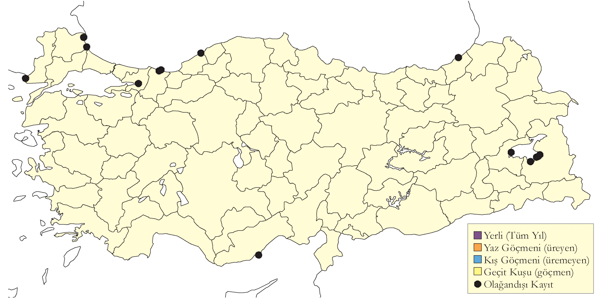
\includegraphics{images/harita_Page_030.png}

\textbf{Üreme}

Türkiye'de yuvalamaz. Kuzey İskandinavya dağlarında ve Rusya ve Kuzey
Amerika'nın tundra kuşağında yuvalar.

\textbf{Alttürler ve Sınıflandırma}

Monotipik bir türdür.

\section{Altıngöz}\label{altux131nguxf6z}

\emph{Bucephala clangula,} Common Goldeneye

\textbf{\emph{Nispeten yaygın ve az sayıda kış konuğudur.}}

Karadeniz, Marmara ve Ege'nin kıyı bölgelerinde ve daha nadir olarak iç
bölgelerdeki sulakalanlarda ekim sonu ve nisan sonu arasında nadir bir
kış konuğudur. En düzenli olarak Marmara ve Karadeniz bölgelerinde
görülür. Kışın ülke çapında görülen kuş sayısı nadiren 100 bireyi geçer.
3 Şubat 1992'de Kızılırmak Deltası'nın açıklarında gözlenen 200 birey
kaydedilen en yüksek sayıdır. 2005-06 kışında Gediz Deltası'nda 72
birey, 3 Şubat 2002'de Gala Gölü'nde 60 birey
sayılmıştır\textsuperscript{67}. Son yıllarda ilkbahar sonunda Doğu
Karadeniz'de kaydedilmiştir.

1977 ile 1993 yılları arasında, Doğu Anadolu'da çoğunluğu Van Gölü'nde
bir dizi yaz kaydı vardır ve bunların bazılarında birden fazla birey
kaydedilmiştir. Bu kayıtlar yakınlarda üreyen bir popülasyonun
ihtimalini düşündürmüştür\textsuperscript{36}.

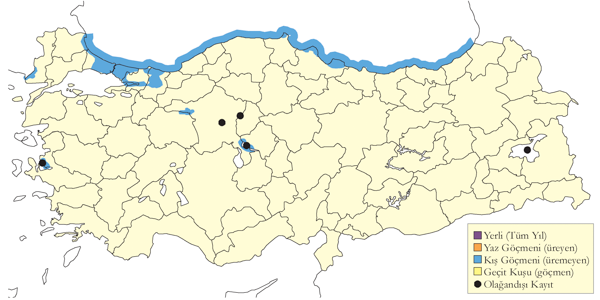
\includegraphics{images/harita_Page_031.png}

\textbf{Üreme}

Türkiye'de yuvalamaz. Avrasya ve Kuzey Amerika'nın kuzeyinde yuvalar.

\textbf{Alttürler ve Sınıflandırma}

Türkiye'de nominat alttürü bulunur.

\section{Sütlabi}\label{suxfctlabi}

\emph{Mergellus albellus,} Smew

\textbf{\emph{Kuzey bölgelerine az sayıda gelen bir kış konuğudur.}}

Kasımdan nisan ortasına kadar ülkenin batı ve orta bölgelerindeki
sulakalanlarda ve kıyılarda tipik olarak nadir ve muhtemelen düzensiz
bir kış konuğudur. En çok Marmara'da, Karadeniz'de ve İç Anadolu'da
kaydedilir. Her kış genellikle 100 bireyden daha azdır. Uluabat Gölü'nde
1967'de 300, 1969-70'de 1300, 1973'te 555, 1989'da 111 ve 1995'de 248
birey kaydedilmiştir. 1992'de Manyas Gölü'nde 102 ve 1993'te
Büyükçekmece'de 79 birey kışlamıştır.

Nisan 1987 sonunda Diyarbakır'da kaydedilmiştir. Doğu ve Güneydoğu
Anadolu'da oluşturulan büyük baraj göllerinde gözlenmesi beklenebilir.
Ocak 1979'da Irak Razzaza Gölü'nde gözlenen 1000'den fazla
birey\textsuperscript{68} daha güneyde yüksek sayılarda
kaydedilebileceğini göstermektedir.

Ancak ne tuhaftır ki, türün ilk keşfi Strickland tarafından İzmir'den
alınan iki örnek ile yapılmıştır. Cambridge Üniversitesi Zooloji
Müzesi'ndeki koleksiyonda bulunan bu örnekler 6 Ocak 1836'da alınan bir
erkek ve aynı yıl şubat ayında alınan bir dişiye aittir. 1946-48
yıllarında Çatalağzı açıklarında (Zonguldak) oldukça bol olduğu
gözlenmiştir\textsuperscript{60}.

11 Haziran 1969'da Eymir Gölü'nde (Ankara) bir erkek\textsuperscript{2},
27 Haziran 1987'de Göründü'de (Van) bir dişi\textsuperscript{9} ve 27
Mayıs 1995'te Uluabat Gölü'nde bir erkek ve iki dişi\textsuperscript{10}
olmak üzere yazın üç defa kaydedilmiştir.

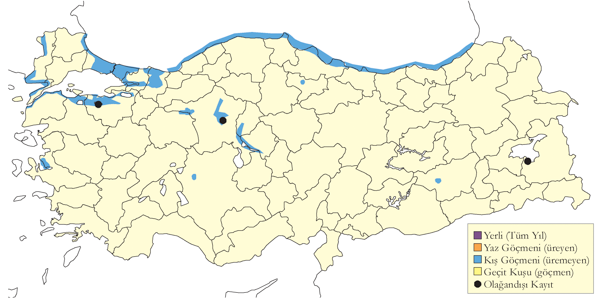
\includegraphics{images/harita_Page_032.png}

\textbf{Üreme}

Türkiye'de yuvalamaz. Avrasya'nın kuzeyinde yuvalar.

\textbf{Alttürler ve Sınıflandırma}

Monotipik bir türdür. Türkiye'de tanımlanmıştır.

\section{Büyük Tarakdiş}\label{buxfcyuxfck-tarakdiux15f}

\emph{Mergus merganser,} Common Merganser

\textbf{\emph{Nadir kış konuğudur.}}

Özellikle Marmara ve Karadeniz bölgelerinde az sayıda kaydedilen nadir
bir kış konuğudur. 1997-2007 arasında artan gözlemci aktivitesine karşın
sadece 10 kere kaydedilmiştir\textsuperscript{6}. Genellikle kıyısal
sulakalanlarda görülür, en düzenli olarak Kızılırmak ve Yeşilırmak
deltalarında kaydedilir. Kızılırmak Deltası'nda görüldüğü en geç tarih
20 Mayıs'tır.

Doğu Anadolu'da şubat ve martta iki defa, yazın üç kere gözlenmiştir; 11
Haziran 1970'de Pasinler ile Horasan arasında Aras Nehri üzerinde bir
çift, 7 Haziran 1986'da Van Gölü'nde bir birey ve 29 Haziran 1988'de
Bendimahi Delta'sında bir dişi ya da genç birey kaydedilmiştir.
Kurutulmadan önce Sevan Gölü (Ermenistan) havzasında üreyen bir tür
olduğu düşünülmüş, ancak ürediğine dair bir kanıt elde
edilmemiştir\textsuperscript{69}.

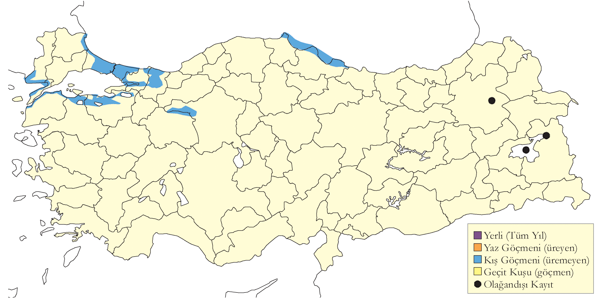
\includegraphics{images/harita_Page_033.png}

\textbf{Üreme}

Türkiye'de yuvalamaz. Avrasya ve Kuzey Amerika'nın kuzeyinde yuvalar.

\textbf{Alttürler ve Sınıflandırma}

Türkiye'de nominat alttürü bulunur.

\section{Tarakdiş}\label{tarakdiux15f}

\emph{Mergus serrator}, Red-breasted Merganser

\textbf{\emph{Nispeten lokal olarak ve orta sayılarda görülen bir kış
konuğudur.}}

Kıyısal alanlarda ekim sonu ve nisan sonu arasında kaydedilen kış
göçmenidir. En çok sayıda Doğu Karadeniz, Marmara ve Ege'de kaydedilir.
Gediz Deltası'nda düzenli olarak yaklaşık 100 birey konaklar, Şubat
1996'da 397 birey sayılmıştır. Büyük Menderes Deltası'nda Şubat 1993'te
67 birey ve Yumurtalık'ta 44 birey kaydedilmiştir. Ege ve Doğu
Akdeniz'deki alanlarda düzenli olarak önemi sayılarda
kışlar\textsuperscript{70}. Akdeniz kıyılarında seyrek olsa da Kıbrıs'ta
oldukça düzenli bir türdür.

20-21 Mayıs 1994'te Göksu Deltası'nda geç kalmış bir birey
kaydedilmiştir (Birdquest Newsletter 23: 59). Tek yaz kaydı 11 Haziran
1964'te Amik Gölü'nde (Antakya) kaydedilen yedi veya sekiz
bireydir\textsuperscript{71}.

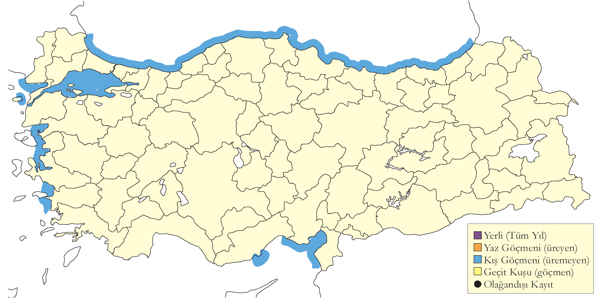
\includegraphics{images/harita_Page_034.png}

\textbf{Üreme}

Türkiye'de yuvalamaz. Avrasya ve Kuzey Amerika'nın kuzeyinde yuvalar.

\textbf{Alttürler ve Sınıflandırma}

Monotipik bir türdür.

\section{Dikkuyruk}\label{sec-dikkuyruk}

\emph{Oxyura leucocephala,} White-headed Duck

\textbf{\emph{Lokal olarak az sayıda üreyen yaz konuğu, nispeten yaygın
ve yüksek sayıda bulunabilen geçit türü ve kış konuğudur.}}

İç Anadolu ve Doğu Anadolu'da tatlı veya acı (sodalı), sığ ve ötrofik
göllerdeki yoğun sazlık sulakalanlarda az ila orta sayıda yuvalar. Van
Gölü çevresinde ve Kars'taki küçük sulakalanlarda ürediği teyit
edilmiştir. Doğu Anadolu'daki diğer alanlardaki üreme durumu
belirsizdir. Niğde Akkaya Barajı'nda üremiştir\textsuperscript{72}.
Üreme döneminde kaydedildiği Karadeniz Bölgesindeki bazı alanlarda
yuvalayabilir. Doğu Akdeniz sulakalanlarında yaz kayıtları üremeyen
bireylere aittir.

1980'lerin sonu ve 1990'ların başı arasında dört kilit alanda (Ereğli
Sazlığı, Hotamış Gölü, Sultansazlığı ve Kulu Gölü) üreyen İç Anadolu
popülasyonu muhtemelen 150 çiftin üzerindeydi. Ancak 1990'ların
ortasında Ereğli Sazlığı ve Hotamış Gölünün kurumasıyla sayıları
azalmış, Kulu Gölünde üremez olmuş\textsuperscript{73}. Kozanlı Gökgöl
ve Uyuz Gölü'nde az sayıda üremeye devam etmektedir.

Mart ile mayıs başı arasında birçok alanda geçiş sırasında gözlenir. 23
Mart 1992'de Kızılırmak Deltası'nda 1246 birey ve Mart 1990'da Ereğli
Sazlığı'nda 508 birey toplanmıştır. Mayıs ve haziran arasında toplanan
sürüler muhtemelen üreme alanlarına dağılacak kuşlardan oluşur. Temmuz
ve eylül arasında toplanan sürüler ise üreme sonrası dağılmaya ve göç
almaya işaret eder. Temmuzda Kulu Gölü'nde 500 birey ve ağustosta Sodalı
Gölü'nde 600-1000 birey kaydedilmiştir.

Kışın Akdeniz'deki birkaç sulakalanda yüksek sayıda, İç Anadolu'da
genellikle daha az sayıda kaydedilir. Batı ve orta bölgelerindeki diğer
yerlerde ise daha nadiren, özellikle sert hava koşullarında kaydedilir.
Karadeniz Bölgesi'nde düzensiz olarak yüksek sayılarda kışlar. Bir dönem
dünya popülasyonunun \%50'sinden fazlasının Burdur Gölü'nde kışladığı
düşünülmüştür; buradaki sayımlarda 1987'de 6400, 1988'de 9230, 1989'da
6700, 1991'de 10.927 birey\textsuperscript{74} kaydedilmiştir. Ancak
1992 sonrasında sayılarda azalma görülmüş; 1992'de 3264, 1993'de 3010 ve
1994'de 3337 birey sayılmıştır. Bu sayımlar son derece hassas olup, eş
zamanlı üç ekip tarafından ideal hava koşullarında gerçekleştirilmiştir.
Burdur Gölü'nde 1993'te 1991'e göre daha az genç bireyin sayılması, daha
düşük üreme başarısını gösterebilir. Bir ihtimal, Kazakistan ve çevre
ülkelerdeki üreyen nüfustaki azalış, Türkiye'deki kışlama nüfusunun
azalmasını açıklayabilir. Bu azalmada şüphesiz kaçak avcılığın da payı
vardır; 1992-93 kışında Burdur Gölü'nde muhtemelen 1000'den fazla
vurulmuştur. Ayrıca son yıllarda Burdur Gölü'nün kuruma sürecinin
başlaması ve tuzluluğun artması da bir etken olabilir.

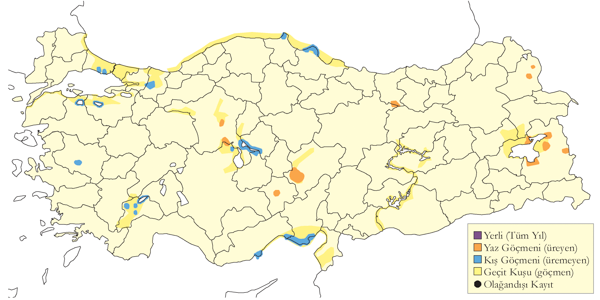
\includegraphics{images/harita_Page_035.png}

\textbf{Üreme}

\textbf{Yuvalama alanı}: Çoğunlukla büyük sulakalanların yakınlarında
genellikle 10 hektardan küçük ve 2 metreden sığ, sualtı vejetasyonu bol
ve su aynalarının bulunduğu geniş sazlıklara sahip olan tatlı su
göllerinde ya da sodalı göllerde ürer\textsuperscript{75}. Aynı alanda
birkaç çift üreyebilir.\\
\textbf{Yuvası}: Yuva, ölü saz gövdeleri ile diğer sucul bitkilerin
düzgün bir kâse oluşturacak şekilde örülmesi ile oluşturulmuş, birkaç
tutam açık gri tüyü ile astarlanmış dayanıklı bir yapıdır.\\
\textbf{Yumurta sayısı}: Bir yuvada en fazla 10 yumurta kaydedilmiştir.
19 Haziran 2004'te aynı gölde diz boyu derinliğindeki suda yoğun bir
sazlığın içinde iyice gizlenmiş bir şekilde suyun üzerinde dikey
sazların dibine tutturularak yapılmış bir yuvada on yumurtalı
tamamlanmış bir kuluçka bulunmuştur. Diğer yerlerde olağan yumurta
sayısı 5-12'dir. Dikkuyruk vücut ölçülerine göre son derece büyük ve
ağır yumurtalar koyar, yuva bu ağırlık nedeniyle suya batabilir.\\
\textbf{Üreme dönemi}: Mayıs başı ve temmuz başı arasında yumurta koyar.
Eylül sonuna kadar yavrular görülebilir. \textbf{İÇA.} 13 Temmuz
1987'de, Kulu Gölü'ndeki sazlıkların içindeki yuvada yedi yumurta
gözlenmiştir; muhtemelen dişinin kuluçkaya ara vermesi nedeniyle yuva ve
yumurtalar kısmen su altında kalmıştır\textsuperscript{75}. Üreme
kayıtlarının çoğu 3-10 yavrulardan oluşan gruplardır: İç Anadolu'daki en
erken kayıt 5 Haziran 1975'te Kulu Gölü'nde gözlenen üç büyük ve üç hav
tüylü yavru olup, yumurtlamanın mayıs başında olduğunu gösterir. 6
Ağustos 1972'de (kurutulmuş) Gönenç Gölü'nde 20 günlük beşer
yavrularıyla iki dişi ve dört günlük altı yavrulu bir dişi gözlenmiştir;
bu kayıtlar yumurtlamanın haziran ortası ile temmuz başında olduğunu
göstermektedir. İç Anadolu'da, temmuz ve ağustosta birçok yavrulu aile
kaydedilmiştir. \textbf{DOA.} Haziran-eylül ayları arasında Van Gölü'nde
9 Haziran 1987 ve 14 Haziran 1990'da gözlenen genç bireyler
yumurtlamanın mayıs ortasında olduğunu göstermektedir. Temmuz-ağustos
arasındaki diğer kayıtlar yumurtlamanın haziran ortasında başladığını
düşündürmektedir. Erçek Gölü yakınlarındaki küçük bir gölün ortasında
dikey sazlardan oluşan bir adada bir yuva bulunmuştur; sucul bitkiler
kullanılarak sazların dibine yapılmış olan yuvada 11 Haziran 2001'de iki
yumurta olduğu, kuluçkanın henüz tamamlanmadığı gözlenmiştir; alanda
sekiz erkek ve yedi dişi birey kaydedilmiştir ancak oldukça esaslı bir
araştırma yapılmasına rağmen başka bir yuva bulunmaması üremenin henüz
tam anlamıyla başlamadığını göstermektedir.

\textbf{Alttürler ve Sınıflandırma}

Monotipik bir türdür.

\bookmarksetup{startatroot}

\chapter{Tavuksular}\label{tavuksular}

\section{Orman Horozu}\label{orman-horozu}

\emph{Lyrurus tetrix}, Black Grouse

\textbf{\emph{Türkiye'de soyu tükenmiştir. Eskiden lokal olarak az
sayıda bulunan yerli türdü.}}

Relikt bir popülasyon 19. yüzyılın sonuna kadar İstanbul çevresinde
devam etmiş\textsuperscript{61}, ancak anlaşıldığı kadarıyla avlanma
sonucunda soyu tükenmiştir. Türkiye'de yaşadığı ilk iki biliminsanı
tarafından tespit edilmiş\textsuperscript{76,77}, son olarak İstanbul
Alemdağ çevresinde bulunduğu düşünülmüş\textsuperscript{78} ve şehirde
satılan ve nereden geldiği bilinmeyen ölü erkek bireyler tespit
edilmiştir\textsuperscript{21}. Aynı dönemde Bulgaristan popülasyonun da
ciddi oranda azaldığını kaydedilmiş\textsuperscript{79}, bu muhtemelen
avcılığa bağlanmıştır. Tür burada da uzun süreden beri tükenmiş
durumdadır. Genel olarak türün küresel yayılış alanı kuzey ve batıya
doğru daralmıştır\textsuperscript{22,80,81} Yunanistan'da 1935 yılından
bu yana Selanik ve Rodop Dağları çevresinden dört kayıt vardır.

\subsection{\texorpdfstring{\textbf{Üreme}}{Üreme}}\label{uxfcreme}

Türkiye'de yuvalamaz. Kuzey Avrasya'daki orman kuşaklarında yuvalayan
yerli türdür.

\textbf{Alttürler ve Sınıflandırma}

Türkiye'de yaşamış popülasyon muhtemelen nominat \emph{tetrix} alttürüne
aittir. Literatürde \emph{Tetrao} cinsi altında da sınıflandırılmıştır.

\section{Dağ Horozu}\label{daux11f-horozu}

\emph{Lyrurus mlokosiewiczi}, Caucasian Grouse

\textbf{\emph{Lokal olarak az sayıda bulunan yerli türdür.}}

Doğu Karadeniz Dağlarının kuzey yamaçlarında bulunur. Ağaç sınırının
üstündeki 1800-3000 metre arasındaki ormangülü (\emph{Rhododendron})
örtüsünde yaşar. 3000 metre üzerinden gelen üreme
kayıtları\textsuperscript{82} doğrulama gerektirir; ancak, neredeyse
yerleşim yerlerine yakın (muhtemelen 15 kilometreye kadar) ve sonbahar
ve kış mevsimlerinde düşük yüksekliklerde bir miktar ağaç sınırının
altında ve muhtemelen özellikle şiddetli soğuklarda daha da düşük
yüksekliklerde bulunurlar. Yayılış bodur ormangülü Rhododendron ile
alpin çayır kuşağının altındaki huş Betula içeren yamaçlar üzerine
yoğunlaşmıştır\textsuperscript{83}.

Artvin'in güneydoğusundan Gürcistan sınırı üzerinde Posof'a kadar
Yalnızçam Dağları'nda dar bir alanda bulunurlar. Yerel halktan alınan
bilgiler ışığında Gümüşhane'nın batısında ve Giresun çevresinde ve
muhtemelen Bingöl'e kadar güneyde, Cilo Dağları'nda bulunması olasıdır.

Türün lokal olarak nadir ya da doğu Karadeniz kıyı şeridi boyunca yaygın
yerli olduğu gösterilene kadar, geçtiğimiz yıllar içerisindeki
kayıtlarda görülen aşırı düzeydeki yetersizlik ile özellikle 1980 öncesi
kayıtlardaki eksiklikler türün Türkiye'de çok az bilinmesine neden
olmuştur. G. Neuhäuser Eylül 1943 tarihinde yüksek olasılıkla Türkiye
için ilk kayıt olan bir çift huş tavuğunu Rize ve Erzurum arasındaki
dağlardan toplamıştır\textsuperscript{28}.

Türkiye popülasyonunun muhtemelen \%90'nın görüldüğü Kaçkar Dağları'nda,
özellikle Sivrikaya çevresinde, 1993 yılında geçekleştirilen gözlem
çalışmalarında kur yapma amacıyla bir araya toplanan (lek poligini) 134
erkek gözlenmiştir. O tarihlerde yapılan tümevarımla toplam popülasyonun
2000 bireyden fazla olduğu tahmin edilmiştir\textsuperscript{57}.
Türkiye popülasyon büyüklüğü son zamanlardaki çalışmalara göre 1508-2675
birey arasında ölçülmüş ve tür 45 coğrafi yerde
kaydedilmiştir\textsuperscript{84}. Bu coğrafi yerlerin 29 tanesi yakın
bir zaman dilimi içerisinde keşfedilmiştir. Bunlardan 4 tanesi nispeten
ayrık popülasyonlardır. Türün yayılış sınırlarını ve popülasyon
büyüklüğünü tam olarak belirlemek için bilgisayar modellemesi
kullanılmıştır\textsuperscript{85}. Ancak, modellemenin sonuçları
bilinen ve yayılış haritasında gösterilen alanını genişletilememiştir.
Bununla birlikte 4900 bireylik popülasyon tahmini önceki en iyimser
tahminlerden bile çok yüksek olmuştur.

Türkiye popülasyonu yaylaların tatil konutlarına dönüşmesi sonucunda
artan yol inşaatları nedeniyle yaşam alanlarının terkedilmesi ile
parçalanmasından etkilenmekte ve nesli tehlike altına girmektedir. daha
az ölçüde avlanma baskısından (özellikle sonbahar döneminde görülen bir
problem) ve Tür için bir tehdit kaynağı olarak listelenen aşırı otlatma
bugün kaydedeğer ölçekte değildir, ancak bu durumun izlenmesi
gereklidir. Türün popülasyonlarının dengede ya da azalmakta olup
olmadığını ortaya koymak için türün popülasyonu ve yayılışı ile ilgili
tarihsel bilgiler yetersiz düzeydedir; ancak, popülasyonların
azalmasından şüphelenir.

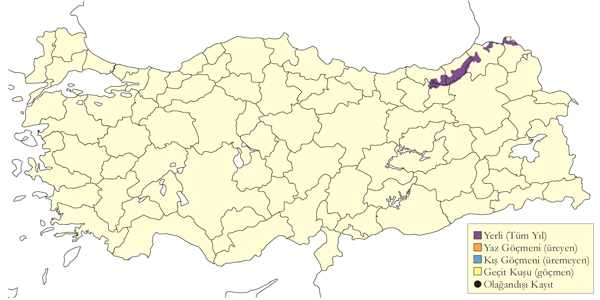
\includegraphics{images/harita_Page_037.png}

\subsection{\texorpdfstring{\textbf{Üreme}}{Üreme}}\label{uxfcreme-1}

\textbf{Yuvalama alanı}:\\
\textbf{Yuvası}: Türkiye'de sadece iki yuva türün en iyi bilindiği
lokalite, Sivrikaya'da (Rize) bulunmuştur. İlk yuva 2800-3000 metrede,
bodur Rhododendron çalılarının bulunduğu 3 hektarlık bir alanda
bulunmuştur. Yuva yoğun, kısa (1 metre) ve çok dallı çallılarda iyice
gizlenmiş olup, kökten çıkan dalların arasında, zeminde sığ bir çanak
şeklinde yapılmış, kuru dallar ve birkaç kuru Rhododendron yapraklarıyla
astarlanmıştır. Bu yuvada 6 Temmuz 1991 tarihinde 5 yumurta
kaydedilmiştir\textsuperscript{86}.\\
\textbf{Yumurta sayısı}:\\
\textbf{Üreme dönemi}:

Erkekler özellikle şafak ve gün batımında, eşeylerin çiftleşme amaçlı
karşılaştığı alanlarda biraraya gelerek bir arada kur gösterileri
(nümayiş) yaparlar. Diğer kayıtlarda dişinin uçarak uzaklaştığı bir
yuvada 12 Temmuz 1993 tarihinde 4 yumurta görülmüş ve bir yumurta kabuğu
11 Haziran 1997 tarihinde bulunmuştur. Bir erişkin dişi ile tam
gelişmemiş iki genç 12 Haziran 2003 tarihinde Ardahan, Posof'da
gözlenmiş ve yumurtlama zamanının mayıs başında başladığını
göstermiştir. Başka yerlerde, yaygın kuluçka küme büyüklüğü 5-6 (2-10)
adettir. Ermenistan'da, 30 Mayıs 1984'de bulunan bir yuva 8 yumurta
içermiş, bu yuvada ilk yumurtanın 21-23 Mayıs 1984 tarihinde bırakıldığı
belirlenmiştir. Bir diğer yuva 20 Mayıs 1985 tarihinde yumurta
içermektedir (ilk yumurta 13-16 Mayıs 1985 tarihinde bırakılmıştır) ve
bir diğeri 31 Temmuz 1994 tarihinde yumurta içermektedir. Bir dişi üç
genç bireyle (ergin büyüklüğünün \%25'ine ulaşmış) birlikte 5 Haziran
1980 tarihinde ve bir diğeri 26 Temmuz 1980 tarihinde tamamiyle büyümüş
5 genç içermektedir (Adamian ve Klem 1999). Ermenistan'dan üreme
döneminin daha erken gösteren kayıtlar Türkiye kayıtlarının normal üreme
dönemini yansıtıp yansıtmadığı hakkında bazı şüpheleri ortaya koymuştur.

\textbf{Alttürler ve Sınıflandırma}

Monotipik bir türdür. Rusca literatürde sıkça görüldüğü gibi, bazen
Lyrurus cinsi altında da sınıflandırılmıştır (farklı uygulamaların özeti
için bkz)\textsuperscript{87}.

\section{Urkeklik}\label{urkeklik}

\emph{Tetraogallus caspius}, Caspian Snowcock

\textbf{\emph{Yüksek dağlarda lokal olarak az sayıda bulunan yerli
türdür.}}

Dağlık alanlarının yerlisidir. Üç önemli popülasyon Doğu Karadeniz
Bölgesi, Yüksekova ile Hakkari'ye ve İran sınırına kadar uzanan Doğu
Anadolu'nun dağlık kısımları ve yukarıda bahsedilen ve en batı sınırını
oluşturan Toroslar olarak belirtilebilir. En batıda Toros silsilesinde
Bolkar ve Melendiz dağlarında kaydedilmiştir. Yaz aylarında genellikle
2400 metrenin üzerinde kaydedilir. Ancak yazın Mersin'in kuzeyindeki
dağlarda 2000 metrenin altında görülmüştür. Ara sıra sonbahar döneminde
60 bireye kadar büyük gruplar oluşturular; bu grupların bazıları kış
ortasında alçak bölgelere inenler olabilir.

Eski kayıtlarda, en batıda Geyik Dağı, Alanya'nın kuzeyi ve Antalya'nın
dağlık alanlarında gözlenmiştir\textsuperscript{28}. Daha batıda
Akdağlar ve Beydağları'ndaki sürekli kar örtüsüne sahip zirveler uygun
yüksekliğe sahip alanlardır.

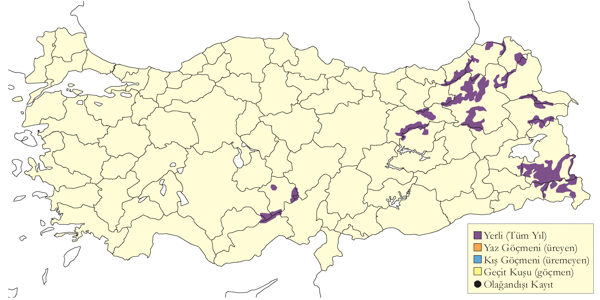
\includegraphics{images/harita_Page_038.png}

\subsection{\texorpdfstring{\textbf{Üreme}}{Üreme}}\label{uxfcreme-2}

\textbf{Yuvalama alanı}:\\
\textbf{Yuvası}:\\
\textbf{Yumurta sayısı}:\\
\textbf{Üreme dönemi}:

Özellikle 2400 metre üzerinde, alpine çayırlarla kaplı, dik kayalıkların
ve yarların olduğu, yıl boyunca karlı ürerler. \textbf{KAR.}
Sivrikaya'da (Rize) beş genç ile bir ergin 12 Haziran 1989 tarihinde
küçük karlı alanları geçerken kaydedilmiştir.
\textbf{AKD.}\textsuperscript{88} Nisan 1876 tarihinde Toroslar
Aladağlar bölgesindeki yuvaları araştırmıştır. Karanfil Dağı'nda 2100
metre yükseklikte 23 Nisan 1876 tarihinde, bir dişi çıkıntılı bir kaya
ve ardıç kökü ile sarılmış bir yuvanın bulunduğu dik bir su yolundaki
küçük bir kaya üzerinden uçmuştur. Yuva taşlı toprak üzerinde derin
yuvarlak bir oyuk olup yetersiz düzeyde kuru otlar ve birkaç kuş tüyüyle
astarlıdır. Bu yuvada altı yumurta kaydedilmiştir. 25 Nisan 1876
tarihinde Bolkar Dağları'ndaki iki yuva benzer özelliklerde
kaydedilmiştir. Ancak bir tanesi yeşil köknar ibreleri ile
astarlanmıştır. Bu yuvalarda altı ve dört yumurta kaydedilmiştir.
Yukarıdaki üç yuvanın ikisinden alınmış iki yumurta Manchester
Müzesi'nde saklanmaktadır. Bu yuvaların ikisinden alınan altı yumurta,
Anadolu'dan 1 Haziran 1894 tarihinde toplanmış ekstra bir yumurta ile 5
Nisan 1901 tarihinde Aladağlar'dan muhtemelen tamamlanmamış bir
kuluçkadan toplanan üç yumurta Tring'deki Doğa Tarihi Müzesi'nde
saklanmaktadır. Son yıllarda, 8 Temmuz 1986 tarihinde Aladağlar'da, 1-2
haftalık 5 genç ile bir ergin gözlenmiş olup, ilk yumurta 21 Mayıs
tarihinde bırakılmış olmalıdır. Çil keklik büyüklüğünde 5-6 ferik ile
bir dişi 3-5 Ağustos 1967 tarihinde (Vielliard 1968) kaydedilmiştir. 19
Ağustos 2000 tarihinde, bazıları erginlerden belirgin derecede küçük 3-4
ferikli en azından üç aile grubu kaydedilmiştir. 6 Ağustos 1966
tarihinde Karanfil Dağı üzerinde 3000 metre yükseklikte iki ergin ve iki
genç kaydedilmişir\textsuperscript{89}.

Ermenistan'da ortalama yumurtlama dönemi 10-15 mayıs arasında, kuluçka
dönemi 20-30 mayıs arasında olup yuvalardan çıkan ferikler 13 Haziran
tarihinde kaydedilmiştir\textsuperscript{69}. Gençlere ait bazı erken
kayıtlar ilk yumurtanın 23 Nisan veya öncesinde bırakıldığını ortaya
koymaktadır. Nisan sonu ile mayıs başını içeren iki kayıt Danford'un
Türkiye'de kaydettiği yuva tarihleri ile kabaca uyum göstermektedir.

\textbf{Alttürler ve Sınıflandırma}

Monotipik bir türdür. Eskiden Hakkari ve Zagros Dağları'ndaki kuşların
\emph{semenowtianschanskii} (Zarudny, 1908), Toros Dağları'nda
\emph{tauricus} (Dresser, 1876) ve Erzurum bölgesinde \emph{challayei}
isimli ayrı alttürlerin olduğu düşünülmüştür.

\section{Kınalı Keklik}\label{kux131nalux131-keklik}

\emph{Alectoris chukar}, Chukar Partridge

\textbf{\emph{Yaygın olarak çok sayıda bulunabilen bir yerli türdür.}}

Yaygın ve Trakya ile Batı Karadeniz kıyı şeridi içerisinde nadir,
Türkiye genelinde oldukça bol yerli bir kuş türüdür. İç bölgelerde
genellikle 700-2000 m arasında görülür. Genellikle kurak, kayalık tepe
ve dağlık alanlarda en az 2800 metreye kadar görülmüştür. Hemen hemen 40
bireye kadar çıkabilen ve gençleri de içeren oldukça büyük sürüler
kaydedilmiştir.

Geçmişte özellikle Hatay ve Doğu Karadeniz kıyı şeridi gibi bölgelerde
oldukça bol olarak kaydedilmiştir. Belirgin bir azalma göstermektedir.

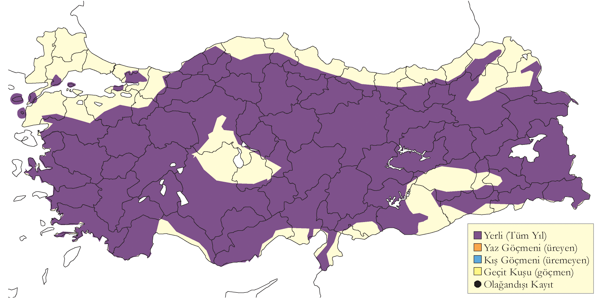
\includegraphics{images/harita_Page_039.png}

\subsection{\texorpdfstring{\textbf{Üreme}}{Üreme}}\label{uxfcreme-3}

\textbf{Yuvalama alanı}:\\
\textbf{Yuvası}:\\
\textbf{Yumurta sayısı}:\\
\textbf{Üreme dönemi}:

Bodur çalılar ile kurumuş tarım alanlarının bulunduğu kayalık ve taşlık
tepelerle oldukça kurak ve çorak alanlarda ürer. Yerde yuvasını bir çalı
ya da bitki dibine gizler. \textbf{EGE.} Kuluçkadaki bir ergin birey
İzmir yakınlarında 14 yumurta içeren bir yuvadan\textsuperscript{90} 7
Mayıs 1951 tarihinde alınmıştır. Yuva yuvanın sahibi olan kuşun çok
sayıda tüyü ile birlikte çalı benzeri bitkilerle astarlanmış ve dikenli
meşe ile de korunmuştur. Yumurtalar krem ile kırmızı arasında bir
renklenme ile kırmızımsı küçük beneklenmeler gösterir
{[}@\textsuperscript{91}1950{]}. \textbf{AKD.} 11 Mayıs 1899 tarihinde
Acıgöl'de 5 yumurtalı bir yuva kaydedilmiştir, dişinin yumurtlamaya
devam edeceği düşünülmüştür\textsuperscript{30}. Karadağ'da, taze
yumurtalar içeren iki yuva 1907 yılının Mayıs sonunda kaydedilmiştir. Bu
yuvada taza yumurtlar haziran ayında da bulunmuştur . Bir ergin ile 5-6
iyi gelişmiş genç birey Burdur ve Bucak arasındaki geçitte 13 Temmuz
1968 tarihinde kaydedilmiştir\textsuperscript{92}. \textbf{İÇA.} 22
yumurta içeren bir yuva 24 Mayıs 1998 tarihinde Ereğli yakınlarındaki
bir kraterin, bir çalı ile sarılmış kaya çıkıntısı üzerinde
kaydedilmiştir. 20 yumurtadan 9 tanesi nisan ayı sonunda bırakılmıştır
(Banoğlu ve Burr 1953). \textbf{DOA.} Nemrut Dağı'nda (Bitlis), 9
Haziran 2004 tarihinde sabah saatlerinde 15 yumurtalı bir yuva
kaydedilmiştir. Ancak, günün ilerleyen saatlerinde, ergin bir birey yuva
üzerine oturmuştur. Muhtemelen bu tarih inkübasyonun ilk günü olarak
belirtilebilir. Yuva kısmen yaprak döken ormandaki bodur çalılar altında
bulunur. Zemine derin bir şekilde kazılmış ve birkaç adet ergin kuş tüyü
ve otların kökleri ile astarlanmıştır. \textbf{GDA.} Kuluçka kayıtları 2
Haziran 2001 tarihinde Işıklı'da (Gaziantep) gençleri içermektedir ve 22
Haziran 1966 tarihinde Menemen (İzmir) yakınlarında 6, 7 ve 8 yavrulu
içermektedir. Akdeniz Bölgesi'nde 22 Mayıs 1989 tarihinde bir kuluçka ve
30 Haziran 1966 Aladağlar'da birkaç günlük genç bir birey
kaydedilmiştir. Birkaç kuluçkanın birleşmesi sonucunda oluşan ve yaygın
olarak gözlemlenmeyen büyük kuluçkalar, tek bir ergin ile birlikte 13
Ağustos 1967 tarihinde Kızılcahamam'da (Ankara)
kaydedilmiştir\textsuperscript{93}.

\textbf{Alttürler ve Sınıflandırma}

Cypriotes alttürü Türkiye'nin güneyi boyunca görülmektedir. Kuzeyde
kleini ve Doğu Akdeniz bölgesine özgü sinaica alttürünün etki gösterdiği
bölgede, Güneydoğu Anadolu'da, kurdestanica alttürü bulunmaktadır. Tür
içerisinde coğrafi varyasyon konusu ile ilgili bir çıkarım yapamadık;
ancak, gözlemlenen formların tamamı güçlü bir şekilde gradient ile
birlikte belirgin klinal yapı göstermektedir\textsuperscript{81}.

\section{Kum Kekliği}\label{kum-kekliux11fi}

\emph{Ammoperdix griseogularis}, See-see Partridge

\textbf{\emph{Güneydoğu Anadolu'da yaygın olarak çok sayıda bulunan
yerli türdür.}}

Son zamanlara kadar çoğu Suriye sınırının 50 km içinde yer alan 15
coğrafi yerde biliniyordu ve 40 bireylik grupların kaydedildiği sonbahar
mevsimi dışında nadiren düşük sayılardan daha fazla kaydedilmişti.
Ancak, Türkiye'nin güneydoğusunda son zamanlarda yapılan gözlemler uygun
habitatların olduğu alanlar ile birlikte türün hemen hemen 50 coğrafi
yerde bulunduğunu göstermiştir\textsuperscript{94}.

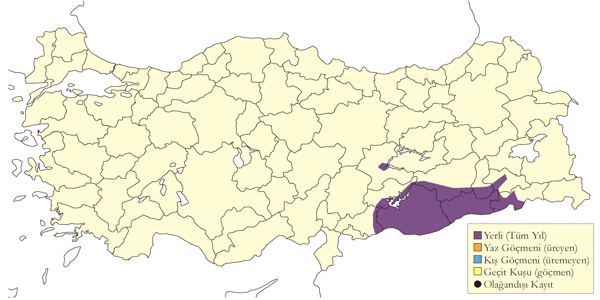
\includegraphics{images/harita_Page_040.png}

\subsection{\texorpdfstring{\textbf{Üreme}}{Üreme}}\label{uxfcreme-4}

\textbf{Yuvalama alanı}:\\
\textbf{Yuvası}:\\
\textbf{Yumurta sayısı}:\\
\textbf{Üreme dönemi}:

Güneydoğu Anadolu'da zayıf vejetasyon örtüsüne sahip kurak kayalık
alanlarda üremektedir. Türkiye içerisinde yuva ve yumurta tanımlaması
yapılmamıştır; ancak, diğer yerlerde, yuvalar yuvanın bulunduğu yere
yakın bitki materyalleri ve otlarla astarlanmış, genellikle taş ya da
bir tutam bitki ile çevrelenmiş şekilde zeminde, toprağa kazılmış halde
bulunur. Kuluçka küme büyüklüğü genellikle 8-12 arasındadır, bazen
yumurta sayısı 16'ya kadar çıkabilmektedir. Nisan ayında çiftler
kaydedilmiştir. 5-7 Haziran 1973 tarihinde Halfeti'de kaydedilen üç
haftalık üç genç birey ile bir ergin, diğer yerlerde kaydedilen ilk
yumurtayı koyma tarihiyle çelişmeyecek şekilde ilk yumurtaların nisan
ortasında bırakıldığını göstermektedir. 2004-05 yıllarında Birecik'te
bir kaç tane genç birey kaydedilmiştir. 11 Ağustos 2001 tarihinde
Cizre'de bir aile kaydedilmiş, gençlerin boyu hakkında detaylar
verilmemiştir.

\textbf{Alttürler ve Sınıflandırma}

Monotipik bir türdür.

\section{Turaç}\label{turauxe7}

\emph{Francolinus francolinus}, Black Francolin

\textbf{\emph{Güneydoğu Anadolu ve Doğu Akdeniz'de yaygın olarak çok
sayıda bulunan yerli türdür.}}

Çukurova ve Göksu Deltaları ve çevresinde, ayrıca Suriye sınırında Fırat
ve Dicle nehirleri boyunca ürer. Doğu Akdeniz popülasyonu en iyi
izlenendir. Çukurova popülasyonunun 75 çiftinin Akyatan Gölü çevresinde
yoğunlaştığı, toplam 85 çifte ulaştığı
kaydedilmiştir\textsuperscript{57}. Göksu Delta'sında, çoğu kumullarda
olmak üzere 50 üreme çifti kaydedilmiştir\textsuperscript{57}. En yaygın
bulunduğu bölge olan Güneydoğu Anadolu'da yaklaşık 15 lokaliteden kaydı
vardır\textsuperscript{95}.

Doğu Akdeniz'deki popülasyonu dikkate alınarak mevcut durumu ve
ekolojisi derlenmiştir\textsuperscript{96}. Doğu Akdeniz'deki bazı
yerlerde tür için koruma tedbirleri uygulanmıştır. Güneydoğu Anadolu'da
ise tarımsal faaliyetlerin artması sonucu hem sayılarının arttığı hem de
yayılış alanının genişlediği düşünülür.

Eskiden Güneydoğu Marmara ile Ege Bölgesi'nin güney kıyılarının bazı
bölümlerinde yerli olarak kaydedilmiştir\textsuperscript{97}. Ancak, her
iki bölgede 19. yüzyıl içinde ortadan kalkmıştır. İstanbul Boğazı
çevresinden 1850'li yıllardan gelen tek bir kayıt vardır. Göller Bölgesi
ile Anti-Toroslara kadar kuzeyde, 600 metreye kadar oldukça lokal olarak
kaydedilmiştir\textsuperscript{28}. Ekim 2003 tarihinde Tavas, Denizli
çevresinden muhtemelen tutsak bir bireyin kaçması sonucu güncel bir
kayıt gelmiştir. 1960'lı yıllarda Köyceğiz Gölü'ndeki kayıtları, Batı
Akdeniz'deki son kayıtlarıdır. 1990'lı yıllara kadar Akdeniz
bölgesindeki yayılışı İçel, Adana, Osmaniye ile sınırlıydı. Sayıları
artan kuşlaırn yavaş yavaş Batı Akdeniz'e doğru ilerlediği
kaydedilmiştir. Örneğin Antalya Havaalanı arazisinde 2010'dan beri
kaydedilir.

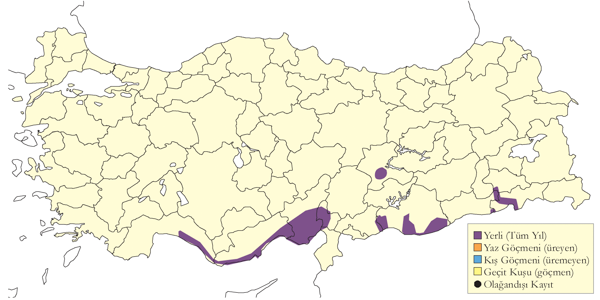
\includegraphics{images/harita_Page_041.png}

\subsection{\texorpdfstring{\textbf{Üreme}}{Üreme}}\label{uxfcreme-5}

\textbf{Yuvalama alanı}: Çalı ve çalı dışındaki bitki örtüsüne sahip
kumullar ile ot, çalı ve bodur bitkilerin arasındaki oyuklarda yaşarlar.
Ayrıca, olgunlaşmamış çalıların bulunduğu nemli (ıslak olmayan) alanlar,
nehir kıyıları ve sık ılgın (Tamarix) çalılarından oluşmuş sık topak
şeklindeki çalılık alanlarda ile mısır tarlalarında ürerler. Kum
tepelerinde (her 2-5 hektarda bir erkek) ve tarım alanlarında (15-30
hektarda bir erkek) yüksek yoğunluktadırlar\textsuperscript{96}.\\
\textbf{Yuvası}: Göksu Deltası'ndaki kum tepelerinde 17 Haziran 1992
tarihinde bulunan eski yuva astarlanmamış, kum içerisinde birkaç bitki
parçasıyla çevrelenmiş sığ bir oyuk şeklinde ve zemininde bir tutam ot
içermektedir.\\
\textbf{Yumurta sayısı}: Türkiye dışında yumurta sayısının genellikle
8-12 arasında olduğu bilinir.\\
\textbf{Üreme dönemi}: Mart sonu ve Nisan arasında yumurta bırakır.
Yavrular mayıs ortasında dolaşmaya başlar. temmuz ortasına kadar
görülebilir. Manchester Müzesi'ndeki üç yumurta (tamamlanmamış bir
kuluçkadan) İzmir yakılarından 10 Mayıs 1899 tarihinde alınmıştır. Tring
Doğa Tarihi Müzesi'ndeki dört yumurtanın ikisi Mersin'den 7 Mayıs 1884
tarihinde ve diğer ikisi 15 Mayıs 1899 tarihinde Anadolu'da bilinmeyen
bir lokaliteden alınmıştır. \textbf{AKD.} Göksu Deltası'ndaki kum
tepelerinde, 17 Haziran 1992 tarihinde muhtemelen bir önceki yıldan
kalmış bir yuva kaydedilmiştir. Yuvada güneşten etkilenmiş ve solgun
renklere sahip yumurta kabukları bulunmuştur. Yuva astarlanmamış, kum
içerisinde birkaç bitki parçasıyla çevrelenmiş sığ bir oyuk şeklinde ve
zemininde bir tutam ot içermektedir. Göksu'da, en azından 1-2 günlük 7
genç ile bir dişi 5 Mayıs 2004 tarihinde kaydedilmiştir. Bu kayıt ilk
yumurtanın 9 Nisan'da bırakıldığını göstermektedir. Bir ergin ile bir
genç kuş 20 Temmuz 1986 tarihinde gözlenmiştir. Çukurova'da, yerel halk
yavruları 10 Mayıs 1986 tarihinde yakalamıştır (yaygın oldukları
bildirilmiştir). Bu tarih yumurta bırakma zamanının yaklaşık nisan
ortasında olduğunu göstermektedir. Ötüşteki artış ise nisan ayının
ikinci yarısı ile mayıs ayının ilk yarısında tepe
yapmaktadır\textsuperscript{96}. Eski avcıların kayıtlarına göre ``dişi
kuşlar mart sonu ile nisan ayı içerisinde yuvaları ve yumurtaları ile
meşguldürler''\textsuperscript{98}. Yumurtalar keklik (kınalı keklik)
yumurtaları büyüklüğünde ve açık yeşil renktedirler; Seyhan ve Ceyhan
kıyılarındaki sık örtüşe sahip bodur ağaçlıklar arasında zemine
bırakılır. Dörtyol ve Alik civarında, dik ve derin vadilerdeki
kayalıkların sınırlarına ya da adalar arasındaki saz yatakları araları
ile bodur ağaçlıklar ve çalı topakları içine yuvalanırlar. Eskiden Adana
civarındaki düzlüklerde çok sayıda görülürlermiş. \textbf{GDA.}
Birecik'in güneyindeki geniş mısır tarlarında ergenlerin sesleri
duyulmuş, üredikleri kesin olarak kaydedilmiştir.

\textbf{Alttürler ve Sınıflandırma}

Türkiye'de nominat alttürü bulunur. Meinertzhagen tarafından Amik Gölü
bölgesinden tanımlanmış \emph{billypayni} alttürü sinonim olarak kabul
edilmektedir.

\section{Çilkeklik}\label{uxe7ilkeklik}

\emph{Perdix perdix}, Grey Partridge

\textbf{\emph{Lokal olarak az sayıda bulunan bir yerli türdür.}}

Tür özellikle ovalardaki tarım alanlarında, uzun boylu ot
topluluklarının kenarlarında ve 2250 metreye kadar birincil yarı step
alanlarda ürerler. Özellikle İç Anadolu ve Doğu Anadolu'nun kuzey
kısımlarında ve Karadeniz Bölgesinin iç kısımlarında yuvalar. Güney
Anadolu'daki yayılış alanının çoğunda çok nadir ve lokaldır.

Geçtiğimiz 20 yıl içerisinde tarımın yoğunlaşması, aşırı otlatma ve
avlanma nedeniyle popülasyonu önemli derecede azalmıştır. Trakya'da
yabani nesli tükenmiş, devlet kurumları tarafından nüfusu takviye
``restocking'' amaçlı genetik yapısı farklı olan yetiştirilmiş kuşlar
salınmış, ancak bunlar yeni bir nüfus oluşturamamıştır. Belki de
Bulgaristan'daki yabani kuşların Türkiye'ye kendiliğinden gelmesi
beklenmelidir.

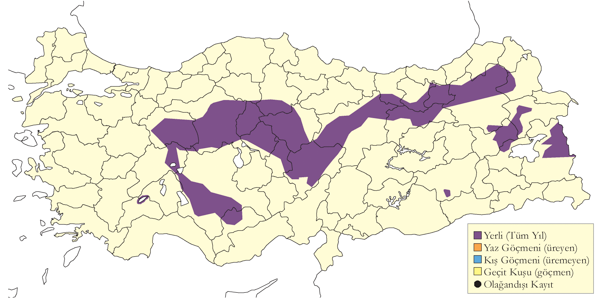
\includegraphics{images/harita_Page_042.png}

\subsection{\texorpdfstring{\textbf{Üreme}}{Üreme}}\label{uxfcreme-6}

\textbf{Yuvalama alanı}: Genellikle açık tarım alanlarında ürer.\\
\textbf{Yuvası}: Türkiye'deki bir yuvası betimlenmemiştir, ancak diğer
yerlerden gelen bilgilere göre yuva ot ve ölü yapraklarla astarlanmış,
genellikle vejetasyon içerisine iyi bir şekilde gizlenmiş ve zeminde yer
alan sığ oyuklar şeklindedir.\\
\textbf{Yumurta sayısı}: 19 yumurta koyabilir. Diğer yerlerdeki yaygın
kuluçka küme büyüklüğü 9-20 (23) arasındadır. Bazen iki dişinin aynı
kuluçkayı paylaşması nedeniyle büyük kuluçkalar da kaydedilebilir.\\
\textbf{Üreme dönemi}: Mayıs ayında yumurtlamaya başlar. Yavrular

\textbf{İÇA.} 11 Haziran 1977 tarihinde bir genç ile bir ergin Mogan
Gölü'nde, 16 Temmuz 1977 tarihinde 8 genç Emir Gölü'nde ve 28 Ağustos
1984 tarihinde 7 bireylik bir aile Çavuşcu Gölü'nde kaydedilmiştir.
\textbf{GDA.} Diyarbakır yakınlarında, 16 Mayıs 1999 tarihinde gevenle
(\emph{Astralagus} sp.) örtülü bir yamaçta on yumurta içeren bir yuva 27
Mayıs'ta 19 yumurta içermiştir\textsuperscript{99}.

\textbf{Alttürler ve Sınıflandırma}

Trakya'da nominat \emph{perdix} alttürü, Anadolu'da \emph{canescens}
alttürü bulunmaktadır. Doğaya salınan değişik orijinden bireylerin yerel
kuşlarla karışması nedeniyle türün yayılış alanı içindeki coğrafi
varyasyonu oldukça karışıktır\textsuperscript{81}.

\section{Bıldırcın}\label{bux131ldux131rcux131n}

\emph{Coturnix coturnix}, Common Quail

\textbf{\emph{Yaygın olarak çok sayıda bulunan bir yaz konuğu ve geçit
türüdür. Nadiren az sayıda kışlar.}}

Çoğunlukla tahıl ekilen kurak tarlalar ve bozkırlarda, çayırlar ve
yüksek otların bulunduğu dağlık bölgelerin yanında yoğun vejetasyonlu
kumullar gibi alanlarda bulunur. Özellikle İç Anadolu'da oldukça yaygın
olarak ürese de hububat tarımının nispeten az olduğu kıyısal bölgelerde
oldukça azdır. Doğu kesimlerinden en azından 2300 metreye kadar
üreyebilir. Üreme ve geçit sırasında özellikle tahıl ekilen arazilerde
bulunur.

Üreme dışında geçit sırasında tüm ülkede bol sayıda bulunur. İlkbahar
geçişi mart sonu ve nisan arasında, sonbahar geçişi ise ağustos sonu ve
eylül boyunca, hatta kuzey bölgelerinde daha da erken olur. Az sayıda
Ege ve Akdeniz kıyılarında kışlar, bu durum geçişin sonunun tespitini
zorlaştırır. Karadeniz kıyılarında da kasıma kadar göçünün sürdüğü
bilinir\textsuperscript{100}. En kuzey bölgelerinde mart sonundan
itibaren görülür. Kasım sonunda 26 Kasım 2003 Seyfe Gölü'nde ve 20 Kasım
2010'da Nallıhan Kuş Cenneti'nde görülmesi geç geçitle
ilgilidir\textsuperscript{101}. Çok az sayıda Batı ve Güney bölgelerinde
kışlayabilir.

Tarım arazilerinde yaşayan diğer kuşlar gibi tarımın yoğunlaşması, tahıl
dışındaki ürünlerin çoğalması ve avcılık sonucunda sayıları ülke çapında
azalmıştır. Göçmen kuşlar aşırı av baskısı altındadır ve özellikle
Karadeniz bölgesinde yasadışı yakalama devam etmektedir.

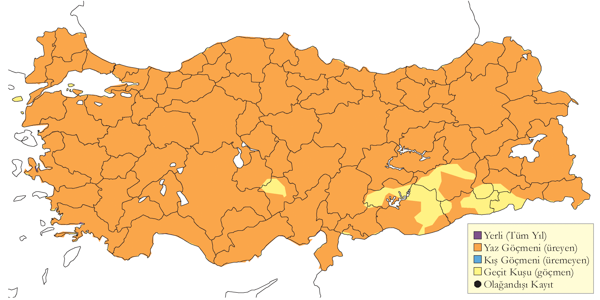
\includegraphics{images/harita_Page_043.png}

\subsection{\texorpdfstring{\textbf{Üreme}}{Üreme}}\label{uxfcreme-7}

\textbf{Yuvalama alanı}: Özellikle hububat tarlalarında yuvalar.\\
\textbf{Yuvası}: Ürediğini kanıtlamak son derece zordur ve Türkiye'de
henüz bir yuvası tespit edilmemiştir. Türkiye dışında; yerdeki düzce bir
çukuru ot ve yakındaki bitkisel materyal ile astarlar.\\
\textbf{Yumurta sayısı}: Genellikle 7-12 arasında istisnai olarak 6 18
arasında yumurta koyar.\\
\textbf{Üreme dönemi}: Genellikle nisan sonu ile mayıs ortası arasında
yumurta koyar. \textbf{MAR.} Uluabat Gölü'nde 22 Mayıs 1966'da yavrular
gözlenmiştir. Çoğu bölgeye ilkbaharda Nisan ortasından gelir ve tüm
yavru gözlemleri üremenin alana varıştan hemen sonra başladığını
gösterir. Ağustos'ta duyulan kuşlar gecikmiş bir üremenin göstergesi
olabilir. \textbf{GDA.} Birecik'te 4 Haziran 1993'de tamamen palazlanmış
3 haftalık 9 yavru, hasat döneminde biçilmiş mısırın altında saklanırken
görülmüş ve köylüler tarafından yenmek üzere yakalanmıştır. 5 Haziran
1993'de görülen başka 6 kuş yumurtlama tarihinin yaklaşık 20 Nisan'da
olduğunu gösterir. Suriye'de yavrularıyla dolaşan bir çift Temmuz'da
gözlenmiştir\textsuperscript{39}.

\textbf{Alttürler ve Sınıflandırma}

Türkiye'de nominat alttürü bulunur.

\section{Sülün}\label{suxfcluxfcn}

\emph{Phasianus colchicus}, Common Pheasant

\textbf{\emph{Lokal olarak az sayıda bulunan yerli türdür.}}

Tüm bilinen tarihi ve güncel lokaliteler
haritalamış\textsuperscript{102}, bu yayılış noktalarının çoğu Güney
Marmara ve Orta Karadeniz'de yoğunlaşmış, en batıda Trabzon'a kadar
doğuya ulaşır.

Doğal ırkı neredeyse tamamen kaybolmuştur, yabani kuşların çoğunun soyu
av için salınan kuşlara dayanır. Toplam stoktaki yerli kuşların varlığı
çok sınırlıdır ve saf yerli kan devamlı olarak av için salınan yabancı
ve karışık kuşların içinde eriyip gitmiştir. Bugün doğal popülasyondan
geriye kalanların Sinop bölgesinde ve yakın zamana kadar Kızılırmak
Deltası ve çevresinde olması olasıdır. İç Anadolu, Ege, Akdeniz'de
görülen sülünler şüphesiz doğaya salma faaliyetleriyle sonucu
oluşmuştur.

Türkiye'deki yerli popülasyonun yayılış alanı büyük ihtimalle Batı ve
Orta Karadeniz kıyısındaki kıyısal ormanlar, ``psödomaki'' olarak
bilinen Akdeniz bitki örtüsü ve fundalıklarla sınırlıydı.

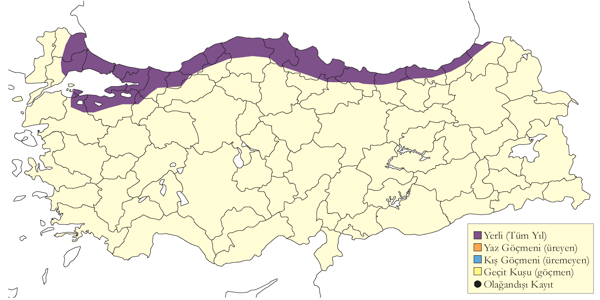
\includegraphics{images/harita_Page_044.png}

\subsection{\texorpdfstring{\textbf{Üreme}}{Üreme}}\label{uxfcreme-8}

\textbf{Yuvalama alanı}: Kıyısal ormanlar, ``psödomaki'' olarak bilinen
Karadeniz kıyılarındaki Akdeniz bitki örtüsü ve fundalıklar..\\
\textbf{Yuvası}: Bu konuda Türkiye'den bir bilgi yoktur. Zemine
yuvalar.\\
\textbf{Yumurta sayısı}: Diğer yerlerde 6-11 yumurta koyar.\\
\textbf{Üreme dönemi}: Diğer yerlerde mayıs ve haziran arasında yumurta
koyar.

\textbf{Alttürler ve Sınıflandırma}

Yerli popülasyon çoğu yazarca nominat \emph{colchicus} alttürü olarak
tespit edilmiş\textsuperscript{103,104}, popülasyonu Kuzey Kafkasya'da
bulunan \emph{septentrionalis} alttürü olarak
tanımlamıştır\textsuperscript{28}. Türkiye yerli bir popülasyonunun
varlığını şüpheli görmüştür\textsuperscript{81}. Ancak İstanbul
bölgesinden 1792'lerden itibaren gelen kayıtlar yerli popülasyonun
varlığını desteklemiştir\textsuperscript{102}.

\bookmarksetup{startatroot}

\chapter{Deniz ve Göl Kuşları}\label{deniz-ve-guxf6l-kuux15flarux131}

\section{Kızıl Gerdanlı
Dalgıç}\label{kux131zux131l-gerdanlux131-dalgux131uxe7}

\emph{Gavia stellata}, Red-throated Loon

{[}Vinyet: Deniz{]}

\textbf{\emph{Nispeten yaygın ancak az sayıda kış konuğudur.}}

Ekim sonu ile haziran başı arasında az sayılarda Orta ve Doğu Karadeniz
kıyılarında görülür. İstisnai olarak kalabalık gruplar oluşturur. 20
tanesi 9 Ocak 1969'da Yeşilırmak ağzında ve 24 tanesi 23 Şubat 2008'de
Kızılırmak Deltası açıklarında gözlenmiştir.

Üremeyen bireyler ilkbahar sonunda ve yazın, genellikle Karadeniz
kıyılarında, daha istisnai olarak iç bölgelerde bulunur. 1 tanesi 14
Haziran 1977'de Van Gölü kıyısında Ahlat'ta\textsuperscript{5}, yaz
giysisinden tüyleri kalmış bir birey 16 Temmuz 2003'de Tödürge Gölü'nde
(Sivas) gözlenmiştir.

Büyük ihtimal İstanbul çevresinden toplanmış iki tahnit İstanbul'da
Saint Joseph Müzesi'nde bulunmaktadır\textsuperscript{59}.

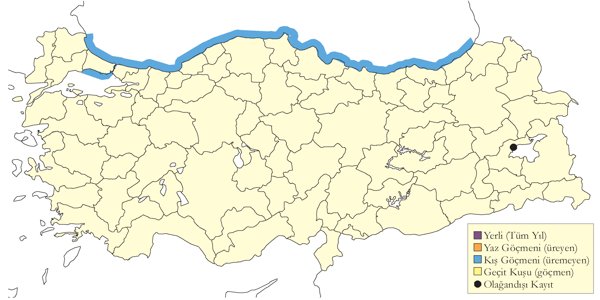
\includegraphics{images/harita_Page_045.png}

\textbf{Üreme}

Türkiye'de ürememektedir. Üreme dönemindeki yayılış alanı K. Kuzey
Amerika ve K. Avrasya'dır.

\textbf{Alttürler ve Sınıflandırma}

Monotipik bir türdür.

\section{Kara Gerdanlı Dalgıç}\label{kara-gerdanlux131-dalgux131uxe7}

\emph{Gavia arctica}, Black-throated Loon

{[}Vinyet: Deniz{]}

\textbf{\emph{Karadeniz'de çok sayıda, diğer denizlerde az sayıda
bulunan bir kış konuğudur.}}

Karadeniz ve Marmara kıyılarında eylül başı ile nisan arasında yaygın ve
bol bulunan kış konuğudur. Orta ve Doğu Karadeniz'de en yüksek sayılarda
görülür. Kışlama döneminin sonuna doğru Karadeniz kıyısındaki kuşların
sayıları güneyden gelenlerin toplanmasıyla artar, şubat sonu nisan başı
arası zirve yapar. Artvin açıklarında 25-27 Ocak 1967'de 1500, 26 Şubat
2006'da 2100 birey kaydedilmiştir. Yeşilırmak Deltası açıklarında 9-10
Ocak 1969'da saatte 50 bireyin batıya uçtuğu gözlenmiştir. Ege ve
Akdeniz kıyılarında oldukça seyrektir, gözlemcilerin yoğun uğradığı
Göksu Deltası, Çukurova sulakalanları ve Hatay'da çok nadirdir. Batı ve
orta kesimlerdeki içsularda nadiren rastlanır. Bunun dışında 1996'da
Ankara Bayındır Barajı, Haziran 1965'te Burdur Gölü, Haziran 2005'te
Aygır Gölü ve Akdeniz kıyısında gözlenmiştir.

Üremeyen kuşlar nadiren Orta ve Doğu Karadeniz kıyılarında yaz aylarında
gözlenebilir, bazı kuşlarda kur davranışı bile gözlenmiştir. Van
Gölü'nde Haziran 1978, Haziran 1983, Temmuz 1987 ve Temmuz 1995'te
gözlenmiş, son kayıt suyun sodalı özelliği nedeniyle tüyleri beyazlaşmış
bir bireye aittir.

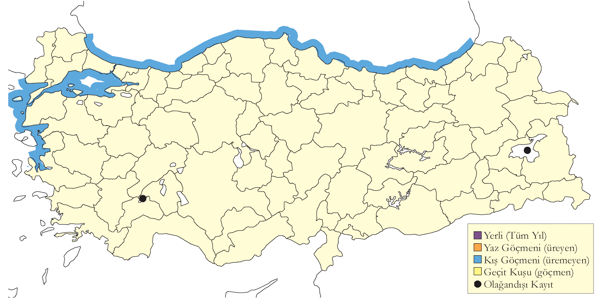
\includegraphics{images/harita_Page_046.png}

\textbf{Üreme}

Türkiye'de ürememektedir. Üreme dönemindeki yayılış alanı K. Avrasya ve
B. Alaska'dır.

\textbf{Alttürler ve Sınıflandırma}

Türkiye'de nominat alttürü bulunur.

\section{Buz Dalgıcı}\label{buz-dalgux131cux131}

\emph{Gavia immer}, Great Northern Loon

{[}Vinyet: Deniz{]} {[}Vinyet: Rastlantısal{]}

\textbf{\emph{Rastlantısal konuktur.}}

Dört güncel kaydı bulunur. Yaz giysisinde bir kuş 13 Mayıs 1964'de
İstanbul Büyükçekmece açıklarında\textsuperscript{105}, bazıları üreme
giysisine girmeye başlamış toplam 8 kuş 29 Nisan 1968'de aynı
yerde\textsuperscript{106}, biri 27 Mart 1981'de Tekirdağ Şerefli Deresi
ağzında\textsuperscript{107} ve ölü bir kuş 13 Mayıs 1989'da Göksu
Deltası'nda\textsuperscript{9} bulunmuştur.

İstanbul Robert Kolej'de bulunduğu söylenen
tahnit\textsuperscript{21,61}1996'daki envanter çalışmasında
bulunamamıştır\textsuperscript{59}. Lakin Robert Kolej'deki birçok
tahnitin 1992'den sonra zarar gördüğü veya yok olduğu bilinmektedir.
Şans eseri Kasparek 1986'daki ziyaretinde bu tahnitin bir fotoğrafını
çekmeyi başarmıştır.

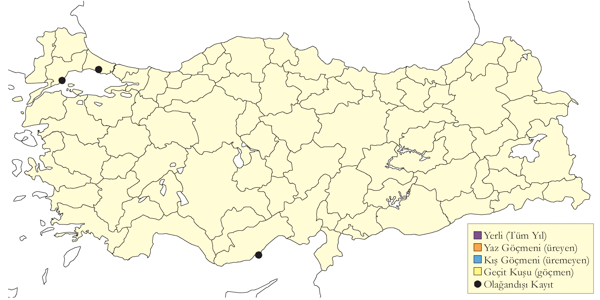
\includegraphics{images/harita_Page_047.png}

\textbf{Üreme}

Türkiye'de ürememektedir. Üreme dönemindeki yayılış alanı K. Kuzey
Amerika ve K. Avrasya'dır.

\textbf{Alttürler ve Sınıflandırma}

Monotipik bir türdür.

\section{Boz Yelkovan}\label{boz-yelkovan}

\emph{Calonectris diomedea}, Scopoli's Shearwater

{[}Vinyet: Deniz{]}

\textbf{\emph{Nispeten yaygın ve orta düzeydeki sayılarda bulunan yerli
ve yarı göçmen bir türdür.}}

Krüper zamanından beri birçok araştırmacı Ege ve Akdeniz kıyılarında
ürediğini düşünmüştür. Birkaç noktada çok az sayıda üreyebilir.

Mart başından ekim ortasına kadar oldukça yaygın bir yaz konuğudur.
Sayıları orta düzeydedir. Eylül sonunda daha kalabalık gruplar
oluşturur, Çanakkale Bademli ile Midilli arasında ağustosta bir saatte
batıya uçan 65 tane sayılmış, İzmir'in güneyinde eylülde ve Bodrum
Yarımadası'nda haziran ve temmuzda 50'lik gruplar görülmüştür. Çanakkale
Boğazı'nda 10 Mart 2001'deki 100 kuş sayılmıştır. Marmara Denizi'nde
düzensizdir, İstanbul Boğazı'nda sonbaharda iki kez, Rize'de
yelkovanlarla beraber bir kez tespit edilmiştir.

Kışın mevcut kayıtların aksine sanıldığından daha boldur. İzmir ve
Mersin'den açıklan araştırma teknelerinde bulunan kuş gözlemcisi bilim
insanlarınca 100'lercesi gözlenmiştir.

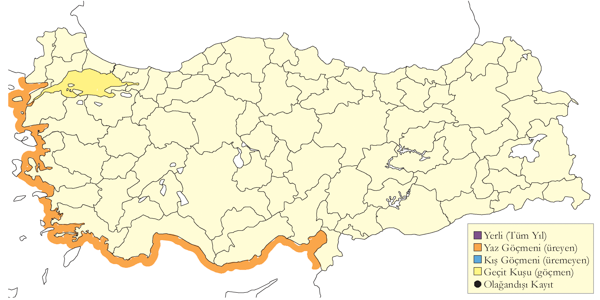
\includegraphics{images/harita_Page_048.png}

\textbf{Üreme}

\textbf{EGE.} 2013 yılında İzmir Seferihisar açıklarındaki bir adada
üredikleri konusunda güçlü kanıtlar toplanmıştır. \textbf{AKD.} Kalkan
ve Kaş arasındaki Heybeliada'da 2010 Ağustos ortasında akşamüstü kıyıya
yakın gözlenen sürüler, adada bir üreme kolonisi olduğunu
düşündürmüştür.

\textbf{Alttürler ve Sınıflandırma}

Monotipik bir türdür. Cabo Verde adalarında üreyen \emph{edwardsii} ve
Azorlar, Madeira\hyperref[_msocom_1]{{[}CO1{]}}~, Kanarya Adaları ve
Portekiz açıklarındaki Berlenga Adaları'nda üreyen \emph{borealis}
taksonları, yakın zamanda tür seviyesine yükseltilmiştir. Bu çalışmadan
önce çıkan birçok kaynakta İngilizce ismi Cory's Shearwater olarak
geçmektedir. Bu İngilizce isim artık sadece Kuzey Atlantik kuşları için
kullanılmaktadır.

\section{Yelkovan}\label{yelkovan}

\emph{Puffinus yelkouan}, Yelkouan Shearwater

{[}Vinyet: Deniz{]} {[}Vinyet: VU (2016){]}

\textbf{\emph{Bütün kıyılarda ve açık denizde yaygın ve çok sayıda
bulunan bir yerli türdür. Kışın gelen göçmenlerle sayıları artar.}}

Karadeniz, Ege ve Akdeniz kıyılarında yıl boyu görülse de sayıları
mevsimsel değişiklik gösterir. Kış sonu ve ilkbahar başında Karadeniz ve
İstanbul Boğazı'nda on binlercesi bir arada bulunur. İstanbul
Boğazı'ndan her gün kalabalık sürülerin geçmesi eskiden beri bir
araştırma konusu olmuştur. 18-22 Nisan 1966'da İstanbul Boğazı'nda
saatte 6800, Çanakkale Boğazı'nda saatte 8200 kuşun her iki yöne uçtuğu
kaydedilmiştir. \hyperref[_msocom_2]{{[}CO2{]}}~3 Şubat 2011'de İstanbul
Boğazı'nda 4 saatte toplam 55.683 birey, aynı yazarlarca Şubat 2012'te
dört saatte toplam 75.000 kuş, ve Şubat 2014'te 90.000 kuş sayılmıştır.
Ege'de kışın daha az sayıda olduğu düşünülür\textsuperscript{70}.
Akdeniz'de nispeten seyrek aralıklarla
rastlanır,\hyperref[_msocom_3]{{[}CO3{]}}~ daha çok mart ve ekim
arasında görülür.

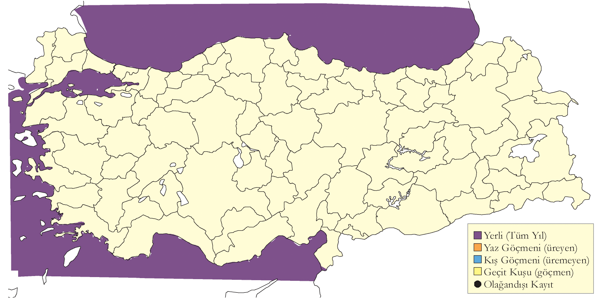
\includegraphics{images/harita_Page_049.png}

\textbf{Üreme}

Ege ve Akdeniz'de kıyıdan uzak adalarda ve kıyıdaki dik yarlarda ürediği
varsayılmış, ancak şu ana kadar ispatlanamamıştır. Türkiye dışında
denize bakan dik yarlarda koloniler halinde ürer, yuvaları yaklaşık 1
metre derinliğindeki oyuklarda veya kaya yığınlarının arasındaki doğal
boşluklarda bulunur. Yuva yatağını döşemek için az ve değişen miktarda
bitkisel materyal kullanır. Nisan ve mayıs arasında tek yumurta bırakır.

\textbf{Alttürler ve Sınıflandırma}

Monotipik bir türdür. Yakın zamana kadar Batı Akdeniz'de üreyen
allopatrik Balear yelkovanı~P. \emph{mauretanicus}~ile aynı tür altında,
30 yıl öncesine kadar Atlantik Yelkovanı'nın \emph{P. puffinus} bir
alttürü olarak değerlendirilmiştir.

\section{Fırtınakırlangıcı}\label{fux131rtux131nakux131rlangux131cux131}

\emph{Hydrobates pelagicus}, European Storm Petrel

{[}Vinyet: Deniz{]}

\textbf{\emph{Ege ve Akdeniz sularında nadir rastlanan bir yaz
konuğudur.}}

Yakın zaman kadar sadece birkaç kaydı olan nadir bir konuk olduğu
düşünülmekteydi. 6 Ağustos 2010'da Didim Açıklarında iki kuş
fotoğraflanmış\textsuperscript{108}, bunu takiben ağustos ve ekim
arasında o sularda düzenli olarak ve Bozcaada ile Kaş arasında az sayıda
kaydedilmiştir.

2010 yılı öncesi kayıtları şu şekildedir: 6 tanesi 15 Mart 1972'de İzmir
Karaada açıklarında, biri 3 Mart 1972'de Kaş açıklarında, 3 tanesi 29
Nisan 1988'de Kaş'ın 10 km batısında\textsuperscript{109} ve 7 tanesi 17
Mart 1992'de gene aynı yerde\textsuperscript{110} tespit edilmiştir.
Karadeniz'den kaydı olduğundan bahseder\textsuperscript{111}.

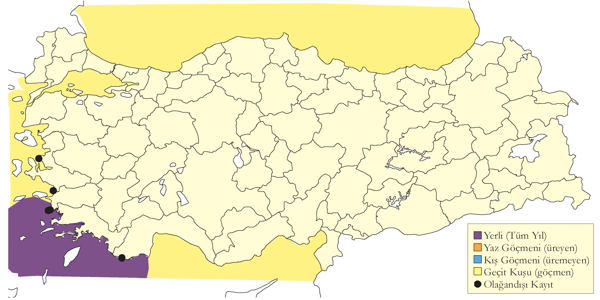
\includegraphics{images/harita_Page_050.png}

\textbf{Üreme}

Yunanistan'ın Ege Adalarında daha önce iki kez ürediği ispatlanmıştır.
Orada muhtemelen düzenli olarak üremektedir (Handrinos ve Akriotis
1997).

\textbf{Alttürler ve Sınıflandırma}

Akdeniz popülasyonu\textsuperscript{112} tarafından tanımlanan
\emph{melitensis} alttürüne aittir. Bu alttür kanat ölçüleri ve ağırlığı
ile nominat alttürden ayrılır.

\section{Küçük Batağan}\label{kuxfcuxe7uxfck-bataux11fan}

\emph{Tachybaptus ruficollis}, Little Grebe

{[}Vinyet: Sulakalan{]}

\textbf{\emph{Yaygın ve çok sayıda bulunan
yerli\hyperref[_msocom_4]{{[}CO4{]}}~ bir tür, aynı zamanda yarı göçmen
ve kış konuğudur.}}

Bataklık sulakalanlarda nispeten az sayılarda ürer. Üreme sonrası
toplanmalara temmuz itibariyle tüm bölgelerde rastlanır. Genellikle
300-500 kuşluk sürüler gözlenirken, Manyas, Erçek ve Van göllerinde
1000'den fazlasının toplanabilir. En yüksek sayı Eylül 2000'de Sarıyar
Barajı'nda kaydedilen 2625 kuştur\textsuperscript{113}.

Kışın çoğunlukla batı ve orta kesimlerdeki tatlı su gölleri,
bataklıklar, göletler, kıyısal sulakalanlar ve az sayıda denizde
görülür. En yüksek sayılarda batı ve güney bölgelerinde, özellikle Bafa
Gölü, Büyük Menderes Deltası, Köyceğiz Gölü ve Göksu Deltası'nda
rastlanır. Marmara Bölgesi'nde kışın boldur: 1120 tanesi 3 Şubat 1991'de
Küçükçekmece Gölü'nde sayılmıştır. Zonguldak Ereğli'de 1970 sonlarında
kuşların ekimin ikinci yarısında geldikleri ve mart sonuna kadar
kaldıkları gözlenmiştir. İç Anadolu ve Doğu Anadolu'dakiler kışın Ege ve
Akdeniz bölgelerine iner ve martta üreme bölgelerine geri dönerler. İç
Anadolu ve Göller Bölgesi'nde ılıman geçen kışlarda yüksek sayılarda
toplanır. 538 tane 11 Şubat 2005'te Sarıyar Barajı'nda, 1155 tanesi 20
Ocak 2005'te Eğirdir Gölü'nde sayılmıştır.

\includegraphics{images/harita_Page_051.png}

\textbf{Üreme}

Sık bitkilerle kaplı tatlı ve acı göller, bataklıklar ve aynası olan
sazlıklar ve eski nehir yataklarında ürer. Üremesi ve yuvalaması için
yeterli bitki örtüsü olduğu sürece çok küçük göletleri bile
kullanabilir.\hyperref[_msocom_5]{{[}CO5{]}}~ Genellikle canlı bitkilere
tutunan yüzer yuva yapar. Yuva sucul bitkiler öbeğinden oluşur ve
ortasında hafif bir çukur vardır.
\hyperref[_msocom_6]{{[}CO6{]}}~Türkiye'de gözlenen yumurta sayısı 4-5
arasındadır. Türkiye dışında yumurta sayısı çoğunlukla 4-6, istisnai
olarak 2-7 olur. Gözlenen yavru sayısı dağılımı şu şekilde olmuştur. 2
yuvada 1, 4 yuvada 2, 2 yuvada 3, 2 yuvada 4, 1 yuvada 5 adet. Daha
düşük yavru sayıları, kayıplardan kaynaklanır. \textbf{MAR.} En erken
yavru 4 Haziran 1996'da İstanbul Belgrad Ormanı'nda görülmüştür. 2
Haziran 2006'da Uluabat Gölü'nde bulunan bir yuvada beş yumurtaya
rastlanmıştır. \textbf{KAR.} Kızılırmak Deltası tür için en önemli üreme
alanıdır. 1992 yılında üreme popülasyonun 350-500 çift olarak tahmin
edilmiş, yer yer seyrek koloniler oluşturduğu ve üreme sıklığının 100
hektarda 25-45 çift olduğu tespit edilmiştir\textsuperscript{44}. 2 tam
yetişmiş yavru 10 Haziran 1995'te, 4 yavru 15 Temmuz 1971'de
görülmüş\textsuperscript{24} ve 1992 yılındaki kapsamlı araştırmada ilk
yavruya 26 Mayıs'ta rastlanmıştır\textsuperscript{44}). \textbf{EGE.} 5
Mayıs 1995'te Bafa Gölü'nde gözlenen dört yavru yumurtlama tarihinin
nisan başı olduğuna işaret eder. \textbf{AKD.} Çukurova'da en erken
gözlem, 4 Mayıs 1987'de tespit edilen hav tüyleri bulunan bir yavrudur
(Van der Have vd., 1988). 18 Mayıs 1970'te Antalya çevresinde iyice
büyümüş yavrular görülmüştür. \textbf{İÇA.} 18 Mayıs 1998'de Uyuz
Gölü'nde ve 19 Mayıs 1998'de Eşmekaya'da 4'er yumurtalı yuvalar
bulunmuştur. Sultansazlığı'nda karayoluna paralel uzanan kanal boyunca
erişkinlerin kuluçkaya yattıkları gözlenmiş, 14 Mayıs 2004'te bir yuvada
5 yumurta görülmüştür 8 Ağustos 1971'de Akşehir Gölü'nde kuluçkada
erişkinler gözlenmiştir. Sultansazlığı'nda en erken yavru 7 Haziran
1982'de kaydedilmiştir\textsuperscript{114}
\hyperref[_msocom_7]{{[}CO7{]}}~. \textbf{DOA.} 19 Haziran 2004'te Erçek
Gölü'nde yumurtlama süreci devam eden bir yuvada 2 yumurta bulunmuş, bir
başka yuvada ise kabuğun kenarında duran yeni çıkmış iki yavru ve
muhtemelen diğer yavruları sırtında taşıyan bir erişkin gözlenmiştir. 18
Ağustos 1972'de Sodalı Göl'de hala kuluçkaya yatan bir erişkin, 25
Haziran'dan itibaren 7 farklı yavru gözlemi olmuştur. Geç tarihli
kayıtların ikinci kuluçkayla ilgili olması yüksek ihtimaldir.
\textbf{GDA.} 7 Haziran 2006'da Birecik'te yumurtadan yeni çıkmış bir
yavru görülmüştür.

\textbf{Alttürler ve Sınıflandırma}

Batı Anadolu'da nominat \emph{ruficollis} alttürü bulunur. Doğu
Anadolu'da \emph{capensis} \hyperref[_msocom_8]{{[}CO8{]}}~ alttürü
olabileceği iddia edilmiştir\textsuperscript{104}. Avrupalı ruficollis
ve Afro-Asyalı \emph{capensis} ve \emph{albescens} alttürlerinin göz
renginin farkıyla rahatlıkla tespit edilebileceğini
belirtmiştir\textsuperscript{115}. Dolayısıyla Roselaar'ın varsaydığı
alttür, \emph{albescens}, hatta Irak'ta bulunan \emph{iraquensis}
olabilir. Doğu Anadolu'daki kuşların hangi alttüre ait olduğu
kesinleştirilmelidir.

\section{Kızıl Boyunlu Batağan}\label{kux131zux131l-boyunlu-bataux11fan}

\emph{Podiceps grisegena}, Red-necked Grebe

{[}Vinyet: Sulakalan{]}

\textbf{\emph{Lokal ve az sayıda bulunan bir yaz konuğu, yaygın ancak
nadir bulunan bir geçit türü ve kış konuğudur.}}

İç Anadolu'da Ereğli Sazlığı veya Sultansazlığı gibi büyük
sulakalanlara, Doğu Anadolu'da küçük ve bataklık sulakalanlarda yuvalar
ve deniz seviyesinden 2250 metre yükseğe kadar çıkar. Bu tip küçük
sulakalanlar nadiren ziyaret edildiği için, gözlem kayıtlarının
oluşturduğu izlenimden daha bol olabilir. Üreme alanlarına varışı martın
üçüncü haftası olup alanlardan ayrılış ekim sonunu bulur.

Üremeyen bireyler veya üremesi başarısız olanlar yazın küçük topluluklar
oluşturabilir. Temmuz 2001 ortasında Sodalı Göl'de 40 tanesi, 9 Haziran
1998'de Eşmekaya Sazlığı'nda 73 kuş (Eken ve Magnin 1999) toplanmıştır.

20. yüzyılın ilk yarısından gelen kayıtlar, eskiden daha yaygın
bulunduğuna işaret eder. 1945-46 yıllarında Mogan Gölü'nde yaklaşık 20
çift üremiştir\textsuperscript{116}. Oysa Mogan Gölü'ndeki son üreme
1998 yılında kaydedilmiştir. Son yıllarda sulakalanların kurutulması
nedeniyle İç Anadolu'da azalmıştır.

Kışın az sayıda Marmara ve Karadeniz bölgelerinde, nadiren içsularda
görülür. 10 tanesi Ocak 1970'de ve 150 tanesi 1-3 Eylül 1980'de Burdur
Gölü'nde sayılmıştır.

\includegraphics{images/harita_Page_052.png}

\textbf{Üreme}

Kenarları sazlık göller, bataklıklar ve göl aynası olan sazlıklarda
ürer. Çoğunlukla büyüyen bir bitkiye tutuşturulmuş yüzer yuvası, çürümüş
su bitkilerinden oluşur ve ortası çukur olan alçak bir yapıdır.
Türkiye'de tek bir yuvada 3 yumurta görülmüş, Türkiye dışında yumurta
sayısı 4-5 arasındadır. Gözlenen yavru sayısı bir kere 3 çoğu kayıtta 1
tanedir. \textbf{AKD.} 12 Nisan 1973'de Karamık Gölü'nde kur davranışı
gözlenmiştir. \textbf{İÇA.} Çeşitli alanlarda nisan sonu ile mayıs
başında kur davranışı gözlenmiştir. 27 Mayıs 1993'de Eşmekaya'da bir
yumurtalı bir yuva ve 20 Mayıs 1998'de iki yumurtalı bir yuva görülmüş,
yumurtlama sürecinin devam ettiği düşünülmüştür. Aynı alanda 21 Haziran
1998'de gelişmiş bir yavru gözlenmiştir. Ereğli Sazlığı'nda 19 Mayıs
1971'de 3 yumurtalı bir yuva bulunmuştur. 13 Temmuz 1977'de Akşehir
Gölü'nde, 17 Temmuz 1986'da Kulu Gölü'nde yavrular kaydedilmiştir.
Sultansazlığı'nda 1982 Ağustos sonunda yavrulara
rastlanmıştır\textsuperscript{114}. \textbf{DOA.} 29 Mayıs 1969'da Van
yakınında ve 1 Haziran 1990'da Çaldıran Gölü'nde yuva yapımına
rastlanmıştır. Kars yakınındaki bir alanda 18 Temmuz 1992'de yuva
yapımı, 27 Haziran itibariyle toplam 6 yavru kaydedilmiştir.

\textbf{Alttürler ve Sınıflandırma}

Türkiye'de nominat alttürü bulunur.

\section{Bahri}\label{bahri}

Podiceps cristatus

Great Crested Grebe

{[}Vinyet: Sulakalan{]}

Yaygın ve çok sayıda bulunan bir yerli tür ve kış konuğudur.

Özellikle İç Anadolu'nun geniş bataklıklı sulakalanlarında ve Doğu
Anadolu'da son derece bol sayıda bulunur. Uluabat Gölü'nde 400 çift,
Kızılırmak Deltası'nda 250-300 çift üremektedir. Küçük batağanın
kullanabildiği küçük gölet ve bataklıkları tercih etmez, ancak baraj
göllerini sıkça kullanır.

Üreme sonrasında ve kışın daha yaygındır ve yüksek sayılarda görülür.
Kışlayan bireyler ekim başında gelirler ve nisan sonuna kadar kalırlar.
Kıyısal bölgelerde, Kızılırmak ve Yeşilırmak deltaları, Küçükçekmece
Gölü, Büyük Menderes Deltası'nda yoğunlaşır, buralarda sert geçen
kışlarda binlercesine rastlanabilir. Karadeniz kıyılarında yüksek
sayılarda gözlenmiştir. Büyük baraj gölleri önemli sayılar barındırır;
Sarıyar'da 5500, Karakaya'da 12.000 ve Keban'da 10.000 tanesi
sayılmıştır. Kış Ortası Su Kuşu Sayımları'nda 2005'de sayılan yaklaşık
31.000 kuş en yüksek değerdir.

\includegraphics{images/harita_Page_053.png}

\textbf{Üreme}

Kıyılarında sazlar olan göllerde ürer. Yuvası sazlara, nilüferlere ve
kısmen su altındaki dalların üzerine kurulur, sucul bitkilerden oluşur,
ortasında sığ bir çukur vardır. Sığ sularda yuvayı su tabanına oturtur,
daha derin yerlerde yüzer yuva bir bitkiye tutturulur. Uluabat Gölü'nde
1998'de üreyen kuşlar, en yoğun olarak yer yer kesintiye uğrayan sazlık
şeridinde görülmüş, alandaki sayısız göl aynası ve kanal kuşların
beslenme ve dinlenme ihtiyaçlarını karşılamıştır\textsuperscript{53}.
Türkiye'de gözlenen yumurta sayısı 4 veya 5'tir. Gözlenen yavru sayısı
1-5 arasındadır. \textbf{MAR.} Uluabat Gölü'nde ortalama yavru sayısı
2,6 (231 yuvada) olarak tespit edilmiştir\textsuperscript{53}. 25 Nisan
2003'de kuluçkaya yatan birçok çift, 19 Haziran 1999'da yetişmiş
yavruyla dolaşan çiftler görülmüştür. 13 Mayıs 2007'da yaklaşık 3
haftalık yavrulara rastlanmış, yumurtlamanın mart sonunda gerçekleştiği
düşünülmüştür. Yuva yapımı 25 Nisan 1970'de gözlenmiş, 2 Haziran 1967'de
biri dört, diğer beş yumurtalı iki yuva bulunmuştur. 23 Nisan 1966'da
yumurtlama süreci devam eden 3 yuva tespit edilmiş, 24 Mayıs 1966'da
sezonun ilk yavrusu görülmüştür. İznik Gölü'nde 6 Haziran 1966'da çok
küçük yavrusu olan dört çift gözlenmiştir.
\textbf{EGE.}\textsuperscript{30} 13 Mayıs 1899'da yaklaşık 20 yuva
bulmuş ve 21 Mayıs ile 21 Eylül arasındaki geniş dönemde yavru
gözlenmiştir. \textbf{KAR.} Kızılırmak Deltası'nda 27 Nisan 1992'de
yumurtalı yuvalara bulunmuş, ilk yavrular 20 Mayıs'ta tespit
edilmiştir\textsuperscript{44}. \textbf{AKD.} Beyşehir Gölü'nde 1 Mayıs
1967'de yuva yapımı tespit edilmiş, 10 Haziran'dan itibaren yavrular
görülmüştür. Göksu Deltası'nda 14 Eylül 1972'de sekiz tane uçamayan iri
yavru gözlenmiştir. \textbf{İÇA.} Hotamış Gölü'nde nisan sonundan
itibaren kuluçkaya yatmıştır\textsuperscript{48}. Diğer alanlarda en
erken yavru 6 Haziran'da gözlenmiştir. \textbf{DOA.} Van Gölü'nde temmuz
ortasında kuluçkaya yatan erişkinler ve 8 Haziran 1975'de ilk yavrular
tespit edilmiştir. Bu, yumurtlama tarihinin mayıs başı olduğuna işaret
eder.

\textbf{Alttürler ve Sınıflandırma}

Türkiye'de nominat alttürü bulunur.

\section{Kulaklı Batağan}\label{kulaklux131-bataux11fan}

\emph{Podiceps auritus}, Horned Grebe (Slavonian Grebe)

{[}Vinyet: Sulakalan{]} {[}Vinyet: VU (2016){]}

\textbf{\emph{Nadir kış konuğudur.}}

Karadeniz ve Marmara kıyısında eylül sonu ve mayıs başı arasında nadiren
rastlanır. 2008'e kadar 21 bilinen kaydı vardır. 2 Ekim 1972'de
Küçükçekmece açıklarında görülen 6 kuş en kalabalık
gruptur.\textsuperscript{60}tarafından Zonguldak Çatalağzı açıklarında
bir kara boyunlu batağanla beraber görülen kuş şubat sonundan 11 Mart
1948'e kadar konaklamıştır.

Karadeniz ve Marmara kıyıları dışında çok nadirdir. Dört tane 29 Ocak
1997'de Balıkesir Ören'de\textsuperscript{6}, birer kuş Şubat 1989'da
Göksu Deltası'nda\textsuperscript{6}, 22 Nisan 1999'da Diyarbakır
Çınar-Göksu Barajı'nda\textsuperscript{99}, 27 Ocak 2008'de Sarıyar
Barajı'nda ve 27 Ocak 2014'de Sapanca Gölü'nde görülmüştür.

Tek bir yaz kaydı vardır: Üreme giysisindeki bir kuş 1 Temmuz 1985'te
Çaldıran'da gözlenmiştir.

\includegraphics{images/harita_Page_054.png}

\textbf{Üreme}

Türkiye'de ürememektedir. Üreme dönemindeki yayılış alanı K. Avrasya,
Kanada ve K. ABD'dir.

\textbf{Alttürler ve Sınıflandırma}

Monotipik bir türdür.

\section{Kara Boyunlu Batağan}\label{kara-boyunlu-bataux11fan}

\emph{Podiceps nigricollis}, Black-necked Grebe (Eared Grebe)

{[}Vinyet: Sulakalan{]}

\textbf{\emph{Lokal ancak çok sayıda olan bir yaz konuğu, yaygın ve çok
sayıda olan geçit türü ve kış konuğudur.}}

Üreme alanlarında nisan ortası ve ağustos arasında bulunur. Koloniler
halinde ürer, yüzlerce çift bir arada bulunabilir. İç Anadolu'da oldukça
nadirdir. Son zamanlarda, örneğin Kulu Gölü'nde\textsuperscript{73},
sayıları ciddi şekilde azalmıştır. Doğu Anadolu'da 2500 m rakıma kadar
genellikle küçük, ötrofik ve bataklık sulakalanlarda ürer. Kars Kuyucuk
Gölü'nde 330 çift bulunur. Üremede başarısız olanlar temmuzda gözde
sulakalanlarda toplanır. Bunlara sonraki 2 ay boyunca üremeyi bitiren
bireyler ve ülke dışından gelenler katılır. Bu topluluklar birkaç bini
bulabilir. Örneğin Acıgöl'de 1800, Kulu Gölü'nde 2000, Erçek Gölü'nde 9
Eylül 2000'de 10.000 kuş (Birding World 1998) ve Sodalı Göl'de 4000-5000
kuş kaydedilmiştir. Doğu Anadolu'da bu tüy döküm alanlarında aralık
başına kadar kalabilir.

Önemli sayılarda kışlar. Karadeniz ve Marmara kıyılarında lokal olarak
korunaklı koylar ve limanlarda düzenli olarak ekim ortası ile nisan
ortası arasında görülür (Albrecht 1986). Kışlama bölgelerinde mayıs
başına kadar kalabilir. Yüksek sayılarda Göller Bölgesi'nde bulunabilir.
Burdur Gölü'nde düzenli olarak 5000 tanesi, Ocak 1970'de 18.662 tanesi
sayılmıştır. İç Anadolu'da az sayıda kışlar. Son yıllarda Kış Ortası Su
Kuşu Sayımlarında ülke toplamı 2000 kuşun altına inmiştir.

\includegraphics{images/harita_Page_055.png}

\textbf{Üreme}

Sazlıkların ve sualtı bitkilerinin bulunduğu sığ tatlı veya acı göllerde
yuvalar. Genellikle küçük koloniler oluşturur, ara sıra tek başına da
ürer. Yüzer yuvası bir sucul bitkiye iliştirilir. Sucul bitkilerden
oluşan alçak bir öbektir ve ortasında sığ bir çukur bulunur. Türkiye'de
gözlenen yumurta sayısı 1-6 arasındadır ve yumurta sayısının dağılımı,
16 yuvada 1, 11 yuvada 2, 8 yuvada 3, 5 yuvada 4 1 yuvada 5 ve 1 yuvada
6 adet olmuştur. \textbf{MAR.} Uluabat Gölü'nde 20 Haziran 1999'da 1-2
haftalık yavrularını gezdiren birkaç çift, yumurtlama tarihinin 21 Mayıs
civarında olduğunu gösterir. \textbf{KAR.} Kızılırmak Deltası'nda Mayıs
1992'de kur davranışı tespit edilmiş, 11 Mayıs'ta muhtemel bir yuvadan
kalkan bir kuş, düşmanı alandan uzağa sürme davranışı
göstermiştir\textsuperscript{44}. \textbf{AKD.} Çukurova
sulakalanlarında 14 Nisan 1987'de kur davranışı (van der Have vd. 1988),
Karamık Gölü'nde 18 Temmuz 1972'de yavrusu olan iki çift, 29 Temmuz
1972'de Seyhan Barajı'nda üç yavrulu bir erişkin gözlenmiştir.
\textbf{İÇA.} Kulu Gölü'nde 13-15 Temmuz 1971'de bulunan koloni yüzen su
bitkilerinin (Ruppia spec., Scirpus spec. ve Phragmites communis)
oluşturduğu küçük bir adanın kenarında yer almıştır. Toplam 120 yuva
bulunmuş, sadece 42 yuvada yumurtaya rastlanmış, kalanında yumurtadan
çıkmış yavruların yuvayı terkettiği düşünülmüştür. 22 Temmuz 1971'de
Kulu Gölü'nde bulunan 13 yuvada yumurta sayısı 2 yuvada 1, 4 yuvada 2, 5
yuvada 3, 2 yuvada 4 adet olmuştur. Bir yanda yüzen yavrular, diğer
yanda yuva yapan erişkinler gözlenmiştir (Kasparek 1987a). Mogan
Gölü'nde nisan başından itibaren yaz konuğudur, nisan ortasında
çiftleşmiş ve kur yapanlar gözlenmiştir (Wadley 1951). Hotamış
Gölü'ndeki iki koloni toplam 20-25 çift kuştan oluşmuştur (Kirwan
1993a). Çöl ve Uyuz Göllerinde 5 çiftin kur yaptıkları 1 Haziran 1991'da
gözlenmiş, 5 Temmuz 1991'de iki yavrulu bir çift görülmüştür. Bunun
dışındaki 3 yavru kaydının en erken 31 Temmuz'dadır. \textbf{DOA.}
Kuyucuk Gölü'nde 18 Temmuz 1992'de 196 yuva sayılmış, 2000'li yıllarda
330 çift üremiştir. Diğer alanlarda en erkeni 19 Temmuz olan toplam 3
yavru kaydedilmiştir.

\textbf{Alttürler ve Sınıflandırma}

Türkiye'de nominat alttürü bulunur.

\section{Flamingo}\label{flamingo}

\emph{Phoenicopterus roseus}, Greater Flamingo

{[}Vinyet: Sulakalan{]}

\textbf{\emph{Lokal ancak çok yüksek sayıda üreyen yerli ve yarı göçmen
bir türdür. Ayrıca yaygın ve çok sayıda bulunan bir geçit türü ve kış
konuğudur.}}

Tuz Gölü ve Gediz Deltası türün yuvaladığı iki ana alandır.

Tuz Gölü onlarca yıl yaklaşık 10.000-20.000 çifti barındırarak en önemli
üreme alanı olmuştur. 1969'da ilk kez İç Anadolu'da ürediğinden
şüphelenmiş ve Tuz Gölü'nde araştırmalar başlamış, gölün ortasındaki
küçük bir adada yumurta kabukları bulunmuştur. Mayıs 1969'da 14.000
birey tespit edilmiş ve 1500-2000 kuşun ürediği kanısına varılmıştır.
1970'de 5000 çiftin ürediği bir koloni bulunmuş, 1971'de su seviyesinin
yüksek olması nedeniyle sadece 83 yuva sayılmış, 1972'de 3500 çift,
1973'te 3700 çift, 1974'de yaklaşık 1000 yavru ve yavrularla ilgilenen
2000 erişkin ve 1978'de yaklaşık 5000 çift kaydedilmiştir. Araştırmalara
1978-1991 yılları arasında devam edilmemiştir. 1991 ile 2003 yılına
kadar belirli aralıklarla, 2003 yılından sonra her yıl düzenli hava
uçuşları yapılarak kuşlar sayılmıştır. 1991 yılında havadan yapılan
gözlemde yeni bir yuvalama alnı tespit edilmiş, toplam 11.000 yuva ve
4100 yavru sayılmıştır. 1992'de yapılan benzer bir çalışmada 14.000
yavru kaydedilmiştir\textsuperscript{117}. Devamında yapılan sayımlarda
1997'de 4000, 1998'de 11.400, 1999'da 1200, 2000'de 8000-10.000, 2002'de
4750, 2003'de 3059 ve 2004'de 7312 yavru sayılmıştır. 2005 yılında
11.499 çift ve 3309 yavru, 2006 yılında 13.302 yavru, 2007 yılında 4382
yavru sayılmıştır. Aynı yıl yaşanan kuraklık sonucunda yüzlerce flamingo
yavrusunun henüz palazlanmadan öldüğü belirlenmiştir. 2008 yılında 1610
yavru, 2009 yılında 14.644 yavru, 2010 yılında 5070 yavru sayılmıştır.
2011 ve 2013 yılları arasında Tuz Gölü'nde Akdeniz ve Batı Afrika'da
bugüne kadar gözlenmiş en yüksek sayıya ulaşılmış, sırasıyla 18.418,
20.274 ve 20.292 yavru sayılmıştır. 2014 yılında yavru sayısı 2893'e
gerilemiştir. Bunun 2007'dekine benzer şekilde yaşanan kuraklık
nedeniyle olduğu düşünülmektedir.

Gediz Deltası'nda Çamaltı Tuzlasında ilk 1982'de 100-150 çift üremeye
başlamış, 1987 yılına kadar üreme denemeleri devam etmiş, ancak üreme
başarısı çok düşük olmuştur. 1987-1991 arasında 100-200 çift düzenli
olarak üremiş ve üreme başarısı artmıştır. Sonraki yıllar sayıları
artmaya başlamış, 1995'te toplam 1752 çift
yuvalamıştır\textsuperscript{57,118}. 2000'li yıllarında
gerçekleştirilen koruma çalışmalarının sonucunda flamingo kolonisi hızlı
bir artış göstermiştir; 2003'te 3100 yavru, 2004'te 3000-3500 yavru,
2005'de 4025 yavru, 2006'da 7140 yavru yetişmiştir (Sıkı 2002, Onmuş ve
Sıkı 2011). Üredikleri adaların erozyona uğramaları nedeniyle koloni
küçülmeye başlamış, 2007'de 3000-4000 yavru, 2008'de 3200 yavru, 2009'da
3000-3500 yavru, 2010'daysa 2071 yavru sayılmıştır (Onmuş ve Sıkı 2011).
2011 yılında 2500-3000 çiftin üremesi koloniye giren köpekler nedeniyle
başarısızla sonlanmıştır. Aynı yıl deltada ilk kez Homa Lagününde
başarılı bir şekilde yaklaşık 1000 yavru. 2012 yılında Çamaltı
Tuzlası'nda üredikleri adanın kıyı erozyonuyla yokolması karşısında bir
proje geliştirilmiş, 6.400 m2 büyüklüğünde bir üreme adası inşaat
edilmiştir. Flamingolar 2012 ve 2013 yıllarında bu üreme adasını
kullanmamış, Homa Dalyanı'ndakiler üremeye devam etmişlerdir, 2012
yılında burada 1600 yavru sayılmış, 2013 yılında 3000 çift üremeye
başlamış, fırtınalar nedeniyle yalnızca 130-140 yavru hayatta kalmıştır.
2014 yılında kurulan üreme adası ilk kez başarıyla kullanılmış, deltada
bugüne kadar en büyük koloni oluşmuş; 10.812 çift ve 7000 yavru
sayılmıştır.

1969'dan beri toplam 9 alandan üreme kaydı gelmiştir. Acıgöl'de 1964 ve
1968'de üremiştir\textsuperscript{20}, 1993'te azami 100 çiftlik bir
koloni bulunmuş, 2006'da ise 100 yavru flamingo gözlenmiştir. Akşehir
Gölü 2008 yılında ilk kez tamamen kuruduğunda buradaki koloniye
ulaşılmış ve 100 ölü yavru flamingo tespit edilmiştir. 2013'de 2950-3200
çift kolonide gözlenmiş, ancak üreme sezonunun ilerleyen döneminde
koloninin dağıldığı tespit edilmiştir. 1960'larda az sayılarda Ceyhan
Deltası'nda (muhtemelen Yumurtalık Lagünleri) ürediği
düşünülmüş\textsuperscript{105}. Akyatan Gölü'nde 2009 yılında 163
yuvadan oluşan bir üreme adası tespit edilmiş, ancak koloninin yavru
çıkarıp çıkarmadığı tespit edilememiştir. Sultansazlığı'nda Yay Gölü'nde
1970'te 1500-2000 çiftin ürediği bulunmuş\textsuperscript{119}, Haziran
1974'de 8000 kuş sayılmış ve 200 çiftin yuva kurduğu gözlenmiştir.
Geçmişte Türkiye üreme popülasyonunun çok önemli kısmı Sultansazlığı'nda
toplanmaktaydı. Alana ortalama 20.000-30.000 sayılmış, istisnai olarak
Ekim 1980'de 60.000-80.000 tespit edilmiştir. Seyfe Gölü'nde iki küçük
yuvada 1970'de aktif yuvalar görülmüş\textsuperscript{120}, 1992'de ise
1947 yuva sayılmış (Yarar, M. ve Özesmi, U.), Mayıs 1993'te birkaç yüz
yuva tespit edilmiş, ardından 1994 yazında 240 yavru görülmüştür.
Karapınar Ovası'nda 1976 ve 1977'de 500 çiftlik kolonin olduğu
düşünülmüş (Kılıç 1988, Kirwan 1992d), ancak başarılı bir hiçbir zaman
teyit edilmemiştir. Ereğli Sazlığı'nda 1987'de 35-40 tane büyük
olasılıkla önceki yıl da kullanılmış yuva bulunmuş, ardından 1991'de 217
yuva sayılmış, bunların 68'inde yumurta görülmüş, ancak yapılan bir hava
uçuşunda koloninin terk edildiği gözlenmiştir. 1993'te ise 300 üreyen
çift ve birçok yavru görülmüş, en son 1991 yılında en fazla 20 çiftin
ürediği gözlenmiştir. Ereğli Sazlığı'nın 80 ve 90'lı yıllarda
flamingoların üremesi için cazip hale gelmesi, kuruma sürecinde
tuzluluğun artmasından kaynaklanmış olabilir. Bu türün üreme alanlarını
düzensiz olarak mesken etmesi, biyolojisinde son derece iyi bilinin bir
özelliktir. Üreme alanlarına ulaşımının zor olması nedeniyle gözlemci
aktivitesi ve dolayısıyla veri akışı çok düzensizdir.

Erçek Gölü'nde yaz sonu ve sonbahar başında çoğunlukla erişkinlerden
oluşan ve sayıları binleri bulan topluluklar bulunur. Erçek Gölü, Sodalı
Gölü ve diğer Van Gölü havzasındaki sulakalanlarda görülen kuşlar
muhtemel İran Urumiye Gölü'nden gelirler. İran'da üreyen kolonilerde
halkalanan yavru bireyler Türkiye'de en azından 22 kez
gözlenmişlerdir\textsuperscript{121,122}.

Kış aylarında eylül sonu ile nisan başı arasında Marmara, Ege, Akdeniz
sulakalanlarda oldukça yaygın ve yüksek sayıda bulunur. Büyük çoğunluğu
Gediz Deltası, Büyük Menderes Deltası, Seyhan ve Ceyhan Deltaları'nda
toplanır. Kış Ortası Su Kuşu Sayımlarında 1972'de toplam 25.900 kuş
tespit edilmiş, bunun 19.000 tanesi Akyatan Gölü'nde sayılmıştır.
1999'da toplam 51.755 kuş sayılmış, bunların 18.930'u Akyatan Gölü,
14.889'u Büyük Menderes Deltası ve 15.413'ü Gediz Deltası'na
dağılmıştır\textsuperscript{13}. 2002'de Ege'de Büyük Menderes ve Gediz
deltalarında toplam 29.000 kuş sayılmıştır\textsuperscript{123}.
Flamingoların kışlama popülasyonu 2014'ye kadar bir artış göstermiş,
ortalama popülasyon büyüklüğü 55.000±20.000 kuş olarak hesaplanmıştır.
Bazı kuşlar ılıman kışlarda İç ve Doğu Anadolu'daki sulakalanlarda
kalabilir. Ocak 1969'da Tuz Gölü'nde 1700, Sultansazlığı'nda 2000 tanesi
sayılmıştır.

Türkiye'de üreyen kuşların çoğunun ülke sınırlarında kaldığı, kışın göç
almak suretiyle sayılarının arttığı düşünülmekteydi. Bu büyük oranda
doğru kabul edilse de, Türkiye'de üreyen kuşların bir kısmı da dışarıya
gitmektedir. 2003-2009 arasında Gediz Deltası'nda yavru olarak
halkalanan flamingolar Batı Akdeniz, Kuzey Afrika, Doğu Akdeniz ve Arap
Yarımadası'nda toplam 16 farklı ülkede tespit edilmiştir. Bu kuşların
bir kısmı Gediz Deltası dışında Fransa, İtalya ve Cezayir'deki
kolonilerde başarıyla üremiştir. Benzer şekilde Fransa, İspanya ve
İtalya'da dünyaya gelen flamingolar Türkiye'ye yıl boyunca gözlenmiş,
Gediz Deltası'nda başarılı şekilde üremiştir\textsuperscript{121,124}.

\includegraphics{images/harita_Page_056.png}

\textbf{Üreme}

Tuzlu veya aşırı tuzlu sığ göllerde koloniler halinde yuvalar. Yuva
alanları deniz seviyesinden 1100 m rakıma kadar çıkar. Türkiye'deki
kolonilerdeki kuş sayısı 100 ile 23.000 arasında değişmektedir. Koloni
sığ suda, alçak bir adaya veya kurumuş bir çamur düzlüğüne kurulur. Yuva
çamurdan yapılmış, genellikle 25-40 cm, nadiren 10 cm yüksekliğinde
kesik bir konidir, ters çevrilmiş bir saksıya benzer, zamanla kurur ve
son derece sert bir hal alır. Yuvanın ortası çukurdur, zeminine tüyler
eklenebilir. Tek bir yumurta koyar, yumurtlama dönemi nisan başı ile
haziran ortası arasındadır. Yumurtlama tarihi alandaki su seviyesiyle
ilişkili olabilir. Kuşlar üreme dönemi çok hassas olup rahatsızlık
nedeniyle tüm koloniyi terk edebilirler. Yuvayı terkeden kuşlar o yıl
başka bir alan veya bölgede tekrar yuva kurmaz ve yumurta koymaz.
\textbf{EGE.} Gediz Deltası'ndaki tuzlalarda 1995'te 1450 çift üremiş,
koloninin oluşması 15 Mart'ta başlamış, ancak koloni Mayıs sonunda
terkedilmiştir\textsuperscript{40}. \textbf{İÇA.} En düzenli ürediği ve
büyük koloninin bulunduğu Tuz Gölü son derece zor ulaşılan, aşırı tuzlu
ve yazın tamamına yakını kuruyan bir göldür. Burada 31 Mart 1969'da kur
ve çiftleşme davranışı gözlenmiştir\textsuperscript{119}. 18 Mayıs
1970'de bulunan 5000 yuva sudan 25-30 cm yüksekliğe kurulmuş, yuvaların
yüzde 70'i yumurtalı, 20'si azami 10 günlük yavrulu, 10'u ise boş halde
bulunmuştur. Bu gözlem üremenin nisan başına başladığına işaret
eder\textsuperscript{119}. 24 Mayıs 1972'de hemen hemen her yuvada bir
haftalık yavrular gözlenmiştir. 15 Haziran 1973'te tümü 1-3 haftalık
olan yavrular gözlenmiştir. Bu, yumurtlamanın nisan ortasında başladığa
işaret eder. 11 Haziran 1974'de tespit edilen 30-40 günlük
yavrular\textsuperscript{125} yumurtlama dönemininin nisan başı olduğunu
gösterir. 6 Temmuz 1992'de gözlenen 1000-2000 yavrunun yaklaşık 4
haftalık olduğu, yumurtlama başlangıcının nisan başı olduğu tahmin
edilmiştir. 6 Haziran 1992'de havadan yapılan bir sayımda gölün
güneyindeki adalarda koloninin yeri tespit edilmiş, yürüyen yavrulardan
oluşan flamingo kreşinin koloniden 2-5 kilometre uzakta bulunduğu
gözlenmiştir\textsuperscript{57}. Sığ ve acı bir göl olan Seyfe Gölü'nde
18-22 Haziran 1992 en büyüğü 15 günlük yavrular görülmüş, bu gözlem
yumurtlamanın mayıs başı olduğuna işaret etmiştir. 1993'te 13 Mayıs'taki
ziyarette kolonideki yuvaların hepsinin eski olduğu, 14 Haziran'da ise
200-500 yeni yuvanın yapılmış olduğu, yuvaların bazılarının sudan 40 cm
yukarıda olduğu, çoğunda çamurun henüz kurumadığı, ancak sadece yaklaşık
20 tanesinde yumurta olduğu ve üremenin henüz yeni başladığı tespit
edilmiş, aynı yıl 70-80 flamingo yuvası üzerine bir ak pelikan
kolonisinin yerleştiği gözlenmiştir. Ereğli Sazlığı'nda 10 Mayıs 1987'de
önceki yıla ait olduğu düşünülen 35-40 yuva bulunmuş, alanda suyun tatlı
olduğu bir mevkide 1 Haziran 1991'de üç küçük adada 1100 erişkin ve 227
yuva sayılmış, yuvaların sadece 68 tanesinde yumurta
görülmüştür\textsuperscript{126}. 16-17 Haziran 1993'te dört adada
toplam 300 çiftin ürediği tespit edilmiş, yapılan sayımda yuvaların
17'si boş, 54'ü yumurtalı, 33'ü en büyüğü bir haftalık yavrulu olduğu
tespit edilmiş\textsuperscript{117}, yumurtlamanın en erken 10 Mayıs'ta
başladığına karar verilmiştir. Sultansazlığı'nda 8-10 Haziran 1974'de
200 çiftin yuvalamaya henüz başladığı gözlenmiştir\textsuperscript{125}.

\textbf{Alttürler ve Sınıflandırma}

Monotipik bir türdür.

\section{Küçük Flamingo}\label{kuxfcuxe7uxfck-flamingo}

\emph{Phoeniconaias minor}, Lesser Flamingo

{[}Vinyet: Sulakalan{]} {[}Vinyet: Rastlantısal{]}

\textbf{\emph{Rastlantısal konuktur.}}

10-16 Nisan 2006'da Ereğli Sazlığı'nda bir flamingo grubunun içinde
tespit edilen kuş ilk kaydı oluşturmaktadır. Benzer tarihlerde İsrail'de
de kaydedilmesi, bu kuşun yabani olduğu iddiasını desteklemiştir. Bunun
ardından 30 Ocak - 30 Nisan 2009'da Gediz Deltası'nda, 3 Haziran 2009'da
Kulu Gölü'nde, 22 Nisan 2011'de Kulu Gölü'nde, 21 Ocak 2012'de Enez
Lagünleri'nde, 15 Nisan ve 18 Haziran ve sonrasında 24 Ekim - 2 Kasım
2012 arasında Kulu Gölü'nde ve 26 Nisan ve 11 Mayıs 2014'de ve ardından
2015'te gene Kulu Gölü'nde görülmüştür.

İspanya ve Fransa'da yabani olduğu düşünülen kuşlar defalarca gözlenmiş,
Güneybatı Moritanya'da en az bir kez üremiştir. Avrupa'daki kayıtların
bazılarını doğal yaşam parklarından kaçan kuşlar oluşturur.

\textbf{Üreme}

Türkiye'de ürememektedir. Yayılış alanı Sahra altı Afrika'dır.

\textbf{Alttürler ve Sınıflandırma}

Monotipik bir türdür. Bu tür bazen Phoenicopterus cinsi altına
yerleştirilir.

~\hyperref[_msoanchor_1]{{[}CO1{]}}Burası dahil değildi düzeltilenlere
ama geçerken gözüme çarptı. Yer isimlerini orijinal dillerindeki gibi
yazmayı tercih ediyoruz. Yani Madeira şeklinde.

~\hyperref[_msoanchor_2]{{[}CO2{]}}Bu 1966 tarihindeki gözlenen kuş
sayısı mı, yoksa genel bir bilgi mi? Her durumda cümleyi elden geçirmek
gerekiyor. İstanbul Boğazı iki kere geçiyor.

~\hyperref[_msoanchor_3]{{[}CO3{]}}?? Eğer bu kuşçular arasında oturmuş
bir jargon değilse, cümleyi daha anlaşılacak şekilde yazmak gerekir.
``Akdeniz'de nispeten düzensiz gözlenir'' gibi, ama bu haliyle de çok
içime sinmedi.

~\hyperref[_msoanchor_4]{{[}CO4{]}}??

~\hyperref[_msoanchor_5]{{[}CO5{]}}Bu paragrafı üremeye almak daha iyi
olur.

~\hyperref[_msoanchor_6]{{[}CO6{]}}??

``En eski tarihlisi 7 Haziran 1982'de Sultansazlığı'nda olmak üzere
toplam 4 yavru kaydı bulunmaktadır (Kasparek, 1985)'' mı yoksa yavruya
yılın en erken hangi tarihinde rastlandığı mı söylenmek isteniyor? Eğer
öyleyse cümleyi daha iyi anlaşılacak şekilde yeniden düzenlemek gerekir.

~\hyperref[_msoanchor_8]{{[}CO8{]}}``taksomu'' eklenebilir mi buraya?

\section{Sarı Gagalı Leylek}\label{sarux131-gagalux131-leylek}

\emph{Mycteria ibis}, Yellow-billed Stork

{[}Vinyet: Rastlantısal{]}

\textbf{\emph{Rastlantısal konuktur.}}

2016'e kadar 3 kere görülmüş bir Afrika göçmenidir. 7-20 Mayıs 1962'de
Amik Gölü'nde\textsuperscript{49}, 28 Mayıs 1986'da Göksu
Deltası'nda\textsuperscript{11} ve 18-24 Haziran 2012'de Mogan Gölü'nde
birer genç gözlenmiştir.

1996'dan önce İsrail'de 18 kaydı vardır\textsuperscript{127}. Abu
Simbel, Nasser Gölü ve güney Mısır'da düzenli kış
ziyaretçisidir\textsuperscript{128}. Bir genç Ağustos-Eylül 1995'te
Sharm el Sheikh'de fotoğraflanmıştır (Birding World 8: 292, 335).
Haziran-Temmuz 2002'de Bulgaristan'da\textsuperscript{129} görülmüştür.

\includegraphics{images/harita_Page_058.png}

\textbf{Üreme}

Türkiye'de ürememektedir. Yayılış alanı Sahra altı Afrika'dır.

\textbf{Alttürler ve Sınıflandırma}

Monotipik bir türdür.

\section{Kara Leylek**}\label{kara-leylek}

Ciconia nigra

Black Stork

Yaygın bulunan ancak sayıları orta düzeyde kalan bir yaz konuğu, yaygın
ve çok rastlanan bir geçit türü, lokal ve az sayıda olan bir kış
konuğudur.

Ormanlık veya tepelik arazide lokal olarak bulunan bir yaz konuğudur.
İki farklı habitatta ürer. Birincisi su varlığı açısından zengin,
akarsu, göl veya sulakalanların yakınındaki ormanlık arazilerdir.
İkincisi kurak bölgelerde akarsu boylarındaki dik kayalık yarlardır.
Kocaçay Deltası ve Kızılırmak Deltası gibi alanlarda yüksek yoğunlukta
üreyebilir. Kızılırmak Deltası'nda 50'den fazla çift bulunur. Bilinen
üreme alanlarının dışında temmuz ortası görülmeye başlar.

İlkbahar göçü mart ortasından haziran başına kadar sürer. Göç sırasında
batı ve orta bölgelerde daha sık rastlanır. İstanbul Boğazı'nda Sarıyer
tepelerindeki tek noktadan mart ortası ve mayıs sonu arasında 2006'da
1118, 2010'da 1197, 2011 yılında 1246 kuş sayılmıştır (Üner et al 2007,
İKGT 2010 ve 2011).

Sonbahar göçü ağustosun başından kasım başına kadar sürer, eylül
başından ekim başına kadar yoğundur. İstanbul Boğazı'nda 1973'te tek
noktadan yapılan sonbahar sayımında toplam 8318 kuş sayılmıştır, aynı
dönem en yüksek günlük toplam, 18 Eylül 1978'de sayılan 5333 kuş
olmuştur. Son yıllarda bir günde tek noktadan sayılan en yüksek değer 20
Eylül 1995'te 2588 kuş olmuştur. 2008 yılında 22 Eylül ile 10 Ekim
arasında 6 noktadan yapılan kapsamlı çalışmada toplam 16.647 kuş
sayılmış, bugüne kadar bilinen sayıyı ikiye katlamıştır. Ekim başında
Çukurova'da da görülür. Borçka'da ise nadirdir.

Kızılırmak Deltası, Gediz Deltası ve Çukurova sulakalanlarında ortalama
20 kuşluk küçük gruplar halinde kışlar\textsuperscript{67,70,130,131}.

\includegraphics{images/harita_Page_059.png}

\textbf{Üreme}

Ormanlık bölgelerde ağaçlarda, kurak bölgelerde kayalık yarlarda
yuvalar. Hem yaprak döken hem ibreli yaşlı ağaçları kullanır, yuvası
yerden 2,5-6,0 m yüksektir. Yuva dal ve sopalardan yapılmış sığ çanak
şekilli ve dikkat çeken bir yapıdır. Çerçevesi yosun ve çimenlerle
kaplanır. Yeni yuvalar biraz küçük olabilir, yıllanan yuvalar gittikçe
büyür. Türkiye'de 29 yuvada gözlenen yumurta sayısı 3 veya 4 olmuştur.
Yavru sayısı 2-4 arasında, toplam 10 yuvada ortalama 2,9 olmuştur. Bu
istatistikler değerlendirilirken, yerden yapılan gözlemlerde daha çok
büyük yavruların görülebilmesi, döllenmemiş yumurta veya ölmüş
yavruların çoğunlukla görülmemesi hesaba katılmalıdır. \textbf{KAR.} 13
Temmuz 1972'da Kızılırmak Deltası'nda iki yavru gözlenmiş, 23 Temmuz'da
yapılan izlemede kuşların yuvadan uçmuş olduğu
düşünülmüş\textsuperscript{24}, yumurtalama tarihinin nisanın üçüncü
haftası olduğu tahmin edilmiştir. 1992'de 17 Mart'tan itibaren iskan
edilmiş yuvalar, Nisan sonunda ilk yumurtalar ve 26 Mayıs'tan itibaren
yavrular ve genç kuşlar görülmüş, toplam üreyen popülasyonun 30-35 çift
olduğu saptanmıştır\textsuperscript{44}. \textbf{İÇA.} Ürgüp'te 22 Nisan
1971'de yuvada yumurtalar tespit edilmiş, 3 Haziran'da yuvada üç yavru
gözlenmiştir. Kızılcahamam'da üç yumurtalı bir yuva bulunmuş, ilk
yumurtanın 6 Mayıs 1993'te koyulduğu tahmin edilmiştir. 29 Nisan 2007'de
Aksaray'da içinde yumurta ve küçük bir yavru olan iki yuva bulunmuş,
yumurtlamanın mart sonunda başladığı düşünülmüştür.

\textbf{Alttürler ve Sınıflandırma}

Monotipik bir türdür.

\section{Leylek}\label{leylek}

Ciconia ciconia

White Stork

Yaygın ve çok bulunan bir yaz konuğu ve geçit türüdür.

Yaygın ve bilinen bir yaz göçmenidir. En azından 2200 m rakıma kadar
üreyebilir. Mevcut üreyen popülasyon 7000 ile 30.000 çift
arasında\textsuperscript{36}, 15.000 ile 35.000
çift\textsuperscript{41}arasındadır. 1993 baharında İç Anadolu'da geniş
bir sahadaki popülasyonun 1000 ile 3000 arasında tahmin
etmişlerdir\textsuperscript{132}. üreme popülasyonunu 1960'ların
sonlarından itibaren \%60 azaldığını iddia etmiştir\textsuperscript{29}.
Diğer yandan üç kıyı alanında popülasyonun sabit kaldığı, hatta
bazılarında artmış olabileceğini düşünmüştür\textsuperscript{133}.

Leyleğin doğu nüfusunun büyük çoğunluğu Türkiye üzerinden göç eder.
İlkbahar ve sonbahar göçü, İstanbul Boğazı -- Bursa -- Eskişehir --
Akşehir Gölü -- Konya -- Ereğli -- Pozantı - Adana hattındaki dar bir
koridorda gerçekleşir. Kuşlar zaman zaman hattın batısına kayabilir,
Göksu Deltası'nda 25.000 kuşluk sürüler görülebilmektedir.

İlkbahar göçünde Akdeniz Bölgesi'nde şubat sonunda görülmeye başlar, göç
martın ikinci yarısı yoğundur, mayıs sonuna kadar devam eder. Doğu
Anadolu'da nisan başına kadar görülmez. 15 Mart ile 31 Mayıs 2010
arasında İstanbul Boğazı'nda tek istasyondan toplam 105.204 kuş
sayılmıştır (İKGT 2010). Muhtemelen üremeyen gençlerin geçişleri haziran
ortasına kadar devam eder.

Temmuz ortasında üreme sonrası toplanmalar görülür. Dönüş göçü temmuz
sonunda başlar, ağustos ortasından itibaren kuvvetlenir ve eylül başına
kadar devam eder. Ekim sonu ve hatta kasıma kadar küçük göçmen sürülere
rastlanır. İstanbul Boğazı'ndaki yoğun günler genellikle 13 ile 31
Ağustos arasındadır. 1972'de toplam 338.353 kuş sayılmış, günlük en
yüksek değer 29 Ağustos sayılan 52.954 kuş olmuştur. Dört ayrı günde
toplam 35.000'den fazla kuş sayılmıştır. Borçka-Hopa bölgesinde az
sayıda geçer, 21 Mart-14 Mayıs 1994'te Hopa'da sadece 50 kuş
sayılmıştır. Amik Gölü'ndeki gözlemlerinde yüksek sayılarda
kaydedilmiştir\textsuperscript{38}. Belen Geçidi'nde 1976 sonbaharında
103.576 kuş kaydedilmiş\textsuperscript{134}, bu çalışmada geçiş
koridorunun çok daha geniş olduğu ve Akıntı Burnu'ndan Dörtyol'a kadar
uzandığı düşünülmüş, daha güncel gözlemlerde bu teyit edilmiştir.

Az sayıda ılıman bölgelerde kışlayabilir.

\includegraphics{images/harita_Page_060.png}

\textbf{Üreme}

Çoğunlukla küçük ve orta boylu yerleşimlerde, ara sıra da yerleşim
yakındaki ağaçlıklar veya terkedilmiş çiftlik ve binalarda yuvalar.
Yuvası çatı, baca, telefon direği veya elektrik direğine kurulur.
Yuvalaması için yerleştirilen platformları kullanır. En sık yuvaladığı
ağaçlar kavak, söğüt, çam, zeytin ve ardıçdır. Balıkçıl kolonilerinde
yuvaladığı da gözlenmiştir. Yuva dal ve sopalardan yapılmış, çim ve
toprak sıvamış, çukuru çöp, tüy ve çim ile kaplanmış sığ bir çukurdur.
Uzun yıllar kullanılmakta olan yuvalar çok büyük olabilir. Yuvaların alt
kısmına serçe ve söğüt serçesi yerleşebilir, tek bir leylek yuvasının
içinde 50'ye yakın serçe yuvası sayılabilir. Türün üreme biyolojisi Batı
ve İç Anadolu'da iki alan ayrıntılı olarak çalışılmıştır (Göcek~vd.
2010). Türkiye'de tek bir yuvada gözlenen yumurta sayısı 5'dir. Gözlenen
yavru sayısı 5 gözlemde 2, 7 gözlemde 3, 4 gözlemde 4, bir gözlemde 5
adet olmuştur. \textbf{MAR.} Marmara ve Ege'deki bir çalışmada sayılan
yaklaşık 170 yuvanın çoğu köylerin içinde bulunmuştur. Uluabat Gölü'nde
25 Nisan 2003'te kuluçkada gözlenmiş, büyümüş yavrular temmuz sonunda
görülmüştür. \textbf{KAR.} Kızılırmak Deltası'nda 26 Temmuz 1971'de 22
yuvada 55 yavru sayılmıştır. 1975 yılında 3 Mayıs'ta kuluçkadaki ilk
erişkin, 7 Haziran'da ilk yavru gözlenmiştir. 1992'de yuvaların bir
kısmı evlere yakın ağaçlara, bir kısmı dağınık koloniler halinde
korulara dağılmıştır. İlk yavrular 21 Mayıs'ta
görülmüşler\textsuperscript{44}, yumurtlama tarihinin 20 Nisan olduğu
hesaplanmıştır. Toplam popülasyon 125-130 çift olarak tahmin
edilmiştir\textsuperscript{44}. Daha sonra yapılan kapsamlı araştırmada
Bafra Ovası'ndaki popülasyonun en azından 900 çiftten oluştuğu
belirlenmiştir. 12 Haziran 2004'te İspir yakınlarında elektrik
direklerindeki yuvalarında yaklaşık 3-4 haftalık yavrular görülmüş,
yumurtlama tarihinin 15 ve 22 Nisan arasında olduğu düşünülmüştür.
\textbf{EGE.} Milet'te (Aydın) 19 Mayıs 1970'de 30 yuvanın çoğunda küçük
yavru gözlenmiş, yumurtlama tarihinin nisan ortası olduğu
hesaplanmıştır. Söke yakınlarında bir köyde 13 Mayıs
1899'da\textsuperscript{30} 50'den fazla yuvanın çoğunda henüz
çatlamamış yumurtalar, kalanında küçük yavrular gözlenmiş, 21 Nisan'dan
sonra kuluçkaya yattıkları kaydedilmiş, yumurtlamanın 11 Nisan'da
başladığı tahmin edilmiştir. \textbf{AKD.} 27 Mart 2000'de Ceyhan'da
kuluçkaya yatan erişkinler tespit edilmiştir. 7 Mayıs 1987'de
Çukurova'daki yuvanın çoğunda kuşların kuluçkada olduğu görülmüş,
haziran sonu ve temmuz başında iri yavrulara rastlamıştır. 1998'de
Beyşehir Gölü, Yeşildağ köyünde en az 21 tane yuva yapan çift görülmüş,
Dalyan yakınında koloni halinde çam ağaçlarında yuva yapan 10-19 çift
sayılmıştır\textsuperscript{135}. \textbf{İÇA.} Çayır veya bataklıklara
yakın yerleşim yerlerini tercih eder\textsuperscript{132}. 1983-84'te
Kızılcahamam'da kayalık bir yarda\textsuperscript{93}, 1992'de Amasya ve
Osmancık arasında bir kayada yuvaladığı kaydedilmiştir. Erişkinler 15
Mart ile 4 Ağustos arasında yuvada rastlanmışlardır. Çoğu kayıt
erişkinlerin nisan sonu ve mayısta kuluçkaya yattıklarını
göstermektedir. 1993'te bölgede yapılan kapsamlı araştırmada çoğu köyde
sadece bir çift, bazılarında birkaç çift, Eşmekaya'da ise 12 çift tespit
edilmiştir\textsuperscript{132}. 14 Mayıs 2004'te bir erişkin küçük
yavrusunu beslerken görülmüş, yumurtlamanın nisan ortasında olduğu
tahmin edilmiştir. 16 Temmuz 1986'da Kızılcahamam'daki bazı yuvalarda
hala yavrular gözlenmiş, bu da yumurtlamanın nisan sonrası olduğuna
işaret etmektedir. 1992'de Kızılcahamam'da budanmış bir ağacın üstünde
yerden sadece 3 metre yüksekte bir yuva gözlenmiştir. 1 Haziran 1975'te
İncesu'da tek bir iğde ağcında 18 yuva sayılmıştır. Çoğu yuva 5 metreden
yüksektir. \textbf{GDA.} 17 Mayıs 1989'da Birecik ile Cizre arasında beş
yuvada yavru görülmüş, yumurtanın nisan ortasında başladığı
düşünülmüştür. 1 Ağustos 1992'de Şanlıurfa ile Diyarbakır arasında bazı
yuvalarda yavrular görülmüş, dolayısıyla yumurtaların mayıs başından
itibaren koyulduğu hesaplanmıştır. \textbf{DOA.} Yuvada ilk yavru 30
Mayıs 1969'da Van Gölü yakınlarında, son yavru ise 4 Ağustos 1974'de
görülmüştür.

\textbf{Alttürler ve Sınıflandırma}

Türkiye'de nominat alttürü bulunur.

\section{Kelaynak}\label{kelaynak}

Geronticus eremita

Northern Bald Ibis

{[}Vinyet: CR (2016){]}

Lokal olarak ve az sayıda bulunan yerli türdür. Soyu tükenmiş olan
yabani popülasyon bir yaz konuğudur.

Bugünkü kuşların çoğunluğu, yabani popülasyonun yaşadığı yerde esarete
alınmış kuşların soyundan gelir. Bu yarı yabani kuşlardan oluşan koloni
Birecik'te yıl boyunca bulunur. Yaz konuğu olan yabani kuşlar şubatta
gelir, temmuz başında üreme alanından ayrılırdı. 1879'ta ilk çift 16
Şubat'ta ve ilk büyük sürü 18 Şubat'ta
gözlenmiştir\textsuperscript{136}.

İlk olarak Haziran 1839'da Ainsworth tarafından bahsedilen bu koloninin
tam olarak yaşı bilinmemektedir. Ainsworth ayrıca Birecik'in 70 km
kuzeydoğusunda Yaylak'ta bir örnek toplamıştır. 1879'da Danford Birecik
kolonisinin kalabalık olduğundan bahseder. Tristram da iki yıl sonra bu
koloni hakkında yazmıştır. Weigold 1911'de 1000'den fazla kuş saymıştır.
1950'lerdeki ziyaretlerde 400-500 kuş tespit edilmiştir. Haziran 1953'te
Kumerloeve 1300 kadar birey saymış, bu rakama büyük ihtimalle yavruları
da dahil etmiştir.

1956'dan 1959'a kadar sıtma ile mücadele etmek adına Fırat boyunca DDT
ve Dieldrin içeren kimyasal tarım ilaçları kullanılmıştır. Aynı zamanda,
tarımsal üretimi büyük bir çekirge sürüsünden korumak adına Sağlık
Bakanlığı'nın dışında Tarım Bakanlığı da bu kimyasal tarım ilaçlarını
kullanmıştır. Bu olayların kelaynak popülasyonuna etkisi bir felaket
derecesinde olmuştur. Kuşların 600-700 bireye denk gelen \% 70'i
zehirlenerek ölmüş, sonraki 10-12 yıl boyunca üreme başarısı sıfıra
yakın kalmıştır. 1965'te 70-75, 1970'te 30 kullanılan yuva sayılmış ve
bu sayı 1972-1973'e kadar 26'ya düşmüştür. 1972-1973 yıllarda WWF (World
Wildlife Fund, Doğal Hayatı Koruma Vakfı) tarafından bir koruma programı
başlatılmıştır. Bu programın amacı, esas koloninin yaşadığı alanı
avcılıktan korumak, çöp ve atıklardan arındırmak, şehre yakın olan
koloninin daha kuzeyde yeni bir bölgeye taşınmasını, kuşların uzman
gözetiminde üremesini ve alana yeniden yerleşmesini sağlamaktı.
Koloninin yeri 1982'de başarıyla değiştirilmiş, kuşlar esarette
beslenmeye ve üretip doğaya salınmaya başlanmıştır. Ancak yeni kurulan
Kelaynak Üretme İstasyonu'nda kalifiye uzmanların çalışmaması ve türün
biyolojik ihtiyaçları hakkında yetersiz bilgi olması nedeniyle üretme
çalışmaları başarılı sonuçlar vermemiştir. Hatta yabani kuşların üreme
başarısı esarette üreyen kuşlarınkinden daha yüksek kalmıştır. 1977-83
arasında esarette üreyen 23-34 sağlıklı yavru doğaya bırakılmış,
bunların büyük çoğunluğu vahşi kuşlarla göç edememiş, sağa sola
dağılmışlar ve soğuk kış boyunca muhtemelen ölmüşlerdir. Proje sonucunda
iyileşmiş üreme koşulları, yabani kuşlardaki düşüşü durduramamış ve
1982'de üreyen çift sayısı 6 çifte düşmüştür. 1989'da koloniye yalnızca
3 birey dönmüştür. Bunların ikisi ya öldürülmüş ya da bir fırtına
sırasında ortadan kaybolmuştur. Sonuçta Türkiye'deki yabani popülasyonun
soyu 1989'da tükenmiş kabul edilmiştir\textsuperscript{137}.

1996-2000 arasında Biyolog Okan Arıhan'ın bakanlık bünyesindeki
çalışmaları sonucunda yarı yabani koloninin içinde hala göçe gidip gelen
bir bireyin olma ihtimali belirdi. 1990-2000 yılları arasında koloninin
tüm olumsuz koşullara rağmen başarılı bir şekilde yılda ortalama 25
yavru ürettiği, bu yavruların çoğunun zamanında kafese alınmaması
nedeniyle koloniden ayrıldıkları ve muhtemelen dağılarak kaybolduklarını
ortaya çıktı. 2000'de popülasyonun 42 kuşa düşmesine rağmen, koloniyi
gözleme ve üreme başarılarını yükseltme amaçlı çalışmaların başarılı
olduğu görülmekteydi. 2002'de 17 genç kuşun başarıyla palazlandığı
kaydedildi .

Fas'taki bilinen son yabani kolonideki kuşların sayılarının azalması ve
2002 yılında Suriye Palmyra'da küçük bir yabani koloninin
keşfedilmesiyle\textsuperscript{138}, Birecik'teki yarı yabani kuşlar
yeniden tür koruma programlarının konusu oldu. 2013'te göç için salınan
toplam beş kuş doğrudan Suriye kolonisinin bulunduğu Palmyra'ya
uçtukları vericiler sayesinde tespit edildi. Ancak göçe devam eden bu
kuşların Ürdün'de bir su kaynağında zehirlendikleri ortaya çıktı. 2016
yılı itibariyle Birecik kolonisi başarıyla üremeye devam etmekte, ancak
Ortadoğu'daki savaş ve kaçak avcılık baskısı nedeniyle kuşlar göçe
salınamamaktadır.

Birecik dışında, Amik Gölü'nde (Antakya) iki örnek
toplamıştır\textsuperscript{139}. Bu kuşlar muhtemelen Suriye veya
Birecik'ten göç eden kuşlardır. 22 Ağustos 1995'te Uludağ'da kökeni
belirsiz bir gencin kaydı vardır\textsuperscript{140}. Bu kuş
Avusturya'dan gelmiş yarı evcil bir kuş, veya Birecik'ten dağılmış yarı
yabani bir genç olabilir.

\includegraphics{images/harita_Page_061.png}

\textbf{Üreme}

Birecik'teki koloni Fırat kıyısındaki dik kayalık yarlarda tür koruma
çalışmaları kapsamında yapılmış suni çıkıntılar ve oyuklarda
üremektedir. Kuşların çoğunluğu Kelaynak Üretme İstasyonu'nda
yuvalarken, bazıları yan vadide, bazı sıradışı çiftler şehre yakın
yarlarda yuva yapmaktadırlar. Yuvası bitki gövdeleri ve köklerinden
oluşan sığ bir yığındır. Genellikle 3-4 yumurtaya yatar. 1969'da
yumurtlama döneminin mart sonunda olduğu ve nisan ortasına kadar sürdüğü
gözlenmiştir\textsuperscript{141}. 5 Mayıs 1870'te 36 yuva gözlenmiş,
yuvalardan 11'i ayrıntılı olarak incelenmiş, dördünde üçer yavru,
dördünde ikişer yavru ve üçünde de birer yavru tespit edilmiştir.
1971'de Mart sonu ile 2 Nisan arasında 12 yuvada, 2-5 Nisan'da 33 yuvada
ve 6-10 Nisan'da 35 yuvada kuluçkaya başladıkları
gözlenmiş\textsuperscript{141}, yumurtlama döneminin nisan başı olduğu
tespit edilmiştir. 1973'te, toplam 23 yuvaya 80 yumurta koyulmuş,
ortalama yumurta sayısı 3,5 olmuş, toplam 21 yavru palazlanabilmiştir.
1974'te ilk kuşlar 21 Şubat'ta gelmişler, 29-30 Martta yaklaşık 45
erişkin sayılmış, fakat 1 Temmuz'da yalnızca 4 erişkin ve 4 yavrunun
kaldığı gözlenmiştir. 30 Mayıs 1975'te 54 erişkin ve 36 yavru
sayılmıştır. Yuvalarda gözlemlenen yavruların büyüklüğüne bakılırsa
1993, 2001 ve 2004'te üreme döneminin zamanlaması çok benzerdir.

\textbf{Alttürler ve Sınıflandırma}

Monotipik bir türdür. Türkiye-Suriye popülasyonu ile Fas popülasyonu
arasında genetik farklılıklar vardır.

\section{Çeltikçi}\label{uxe7eltikuxe7i}

Plegadis falcinellus

Glossy Ibis

{[}Vinyet: Sulakalan{]}

Lokal ve az sayıda bulunan bir yaz konuğu, yaygın ve çok sayıda
rastlanan bir geçit türüdür.

A local and scarce summer migrant and a widespread and common passage
migrant.

Yoğun bataklık sulakalanlarda genellikle az sayılarda ürer. Bilinen çoğu
kolonide 50 çiftten az sayıda yuvalarken, Meriç Deltası'nda yaklaşık 100
çift üremektedir. 1968'de Marmara Gölü'nde 200-300 kuş üremiştir. İç
Anadolu'daki popülasyonu ciddi oranda azalmıştır. 20. yüzyılın
başlarında Antakya'daki Amik Gölü ve 1800'lerde Büyük Menderes
Deltası'nda ürediği bilinir. Uzatılan ilkbahar göçleri üreme durumunun
anlaşılması güçleştirir. Üstelik küçük gruplar, özellikle Karadeniz
Bölgesi'nde üremeden yazı geçirirler.

Göç sırasında lokal olarak yüksek sayılarda kaydedilir. 26 Temmuz
2004'te Meriç Deltası'nda 1200 tanesi veya 27 Nisan 1992'de Kızılırmak
Deltası'ndaki 590 tanesi gözlenmiştir. İlkbahar göçü mart ortasından
haziran başına kadar devam eder, nisanın ikinci yarısında yoğunlaşır,
muhtemelen mayıs başında ikinci bir zirve yapar. Sonbaharda ise ağustos
başından ekim başına kadar gözlenir, çoğunluk eylül ortasına kadar yurdu
terk etmiş olur. Kışın nadiren az sayıda kaydedilebilir.

\includegraphics{images/harita_Page_062.png}

\textbf{Üreme}

Diğer türlerle karışık koloniler halinde içsu göl ve sazlıklarında ve
kıyısal alanlarda ürer. Koloniler bazen yüzlerce kuştan oluşur, ancak
genellikle kolonide 10-30 çift bulunur ve diğer türlerin arasında
azınlıktadır. Ağaç ve çalılıklarda, bazen subasar alanlarda veya geniş
sazlıklarda yuvalar. Yuvası ince dallardan oluşan sığ bir yapıdır, eğer
bir ağaç veya çalılıkta yapılmışsa çimen ve yapraklarla, sazlıklarda ise
sazlarla çevrelenir. Türkiye'de gözlenen yumurta sayısı 3-5 arasında ve
çoğunlukla 4'tür. Gözlenen yavru sayısı 3 veya 4'tür. \textbf{MAR.}
Manyas Gölü'nde ağaçtaki bir yuvada 3 Haziran 1970'te yumurtadan yeni
çıkmış bir yavru ve 4-6 Haziran 1970'te de yaklaşık 2 haftalık üç yavru
bulunmuş\textsuperscript{55}, bu tarihlere göre yumurtlamanın 1-10 Mayıs
arasında gerçekleştiği düşünülmüştür. Uluabat Gölü'ndeki bir ağaçlıkta 6
türün karışık kolonisi içinde 14 çeltikçi yuvası tespit edilmiş, 7
Haziran 1998'de bazı yuvalarda palazlanmış yavrular, diğerlerinde ise
yumurtalar gözlenmiştir\textsuperscript{53}. 3 Haziran 2006'da yine aynı
kolonide en az 40 çeltikçi yuvası sayılmış, yuvaların çoğunun subasar
bir bölgedeki söğüt ağaçlarının alt dallarında olduğu, bazılarının suda
yüzen sazlardan yapıldığı tespit edilmiştir. Çoğu yuvada yumurtadan yeni
çıkmış yavrular gözlenmiş, yumurtaların en geç mayıs başında koyulduğuna
karar verilmiştir. \textbf{EGE.} Marmara Gölü'nde kaşıkçı, küçük
karabatak ve küçük ak balıkçıl ile karışık bir kolonide diğer türlerin
yuvalarında yumurtalar gözlenirken, çeltikçi yuvalarının henüz boş
olduğu tespit edilmiştir {[}@\textsuperscript{91}1950{]}. 13 Mayıs
1899'da İzmir yakınlarındaki karışık bir kolonide hem çeltikçinin, hem
diğer türlerin yuvalarında yumurtlamanın başlamış olduğunu
kaydetmiştir\textsuperscript{30}. \textbf{AKD.} Amik Gölü'nde
sazlıklarda yılanboyun ve diğer türlerle karışık bir kolonide birkaç
çeltikçi çifti bulunduğunu tespit etmiştir\textsuperscript{56}. Buradaki
çeltikçi yuvalarının sazların dibinde olduğunu ve 26 Mayıs 1933'te
yumurtaların yeni koyulmuş olduğu tespit etmiştir. \textbf{İÇA.} 18
Mayıs 1987'de Ereğli Sazlığı'nda balıkçıl ve küçük karabatakla karışık
bir kolonide 12 yuva sayılmıştır. Çoğu yuvada 4, iki yuvada 3 yumurta
tespit edilmiştir. Yuvaların bazılarında yumurtlamanın devam ettiği
düşünülmüştür. 22-25 Temmuz 1971'de Yarma Bataklığı'nda tüyleri çıkmış
birçok yavru gözlenmiştir.

\textbf{Alttürler ve Sınıflandırma}

Monotipik bir türdür.

\section{Kaşıkçı}\label{kaux15fux131kuxe7ux131}

Platalea leucorodia

Eurasian Spoonbill

{[}Vinyet: Sulakalan{]}

Lokal olarak ve az sayıda üreyen yerli bir tür veya yarı göçmendir. Göç
sırasında yaygın ve çok sayıda bulunur. Lokal ve az sayıda olan bir kış
konuğudur.

Düzenli olarak ürediği alanlar Manyas Gölü, Uluabat Gölü, Kızılırmak
Deltası (76 çift) ve Bolluk Gölü'dür. Murat Nehri'nde Bulanık
yakınlarında ve Muş'taki Haçlı Gölü'nde 1980 yazından düzenli olarak
kayıt gelmiş olmasına rağmen, Doğu Anadolu'dan son yıllarda kesin bir
üreme kaydı yoktur. Göller Bölgesi ve İç Anadolu'nun güneyindeki
sulakalanlarda üremesi olasıdır. Son yıllarda hem sayıları, hem de üreme
başarısı giderek azalmaktadır. Manyas Gölü'ndeki izlenen koloninin uzun
süreli bir çöküşe maruz kaldığı tespit edilmiştir. 1966'da 835 çift
sayılmış, 1995'te yaklaşık 200 çift kalmıştır. Bu popülasyon eskiden
sadece yaz göçmeni iken, bazı kuşların kışlamaya başlamasıyla yarı
göçmen bir nitelik kazanmıştır. En azından 1960 sonlarına kadar
Antakya'daki Amik Gölü'nde üremiştir\textsuperscript{52}. 1839'da
Erzurum yakınlarında Karasu Nehri'nde\textsuperscript{142} ve muhtemelen
19. yüzyılda İzmir yakınlarında da ürediği
kaydedilmiştir\textsuperscript{143}.

Göç sırasında genellikle küçük sayılar halinde bulunur. İlkbahar göçü
yoğun olarak nisan başı ile mayıs sonu arasında gerçekleşir. Sonbahar
göçü ise ağustos başında başlayıp ekim başında biter. İki göçte de
İstanbul Boğazı'ndaki gözlem noktalarında nadiren gözlenir. Oysa Belen
Boğazı'nda 6 Ağustos-21 Eylül 1976 arasında toplam 816 kuş
sayılmıştır\textsuperscript{134}. İç Anadolu'daki birkaç sulakalanda
sonbaharda kalabalık sürüler gözlenebilir. Kışın Ege ile Akdeniz kıyı
bölgelerinde azami 60'lık gruplar halinde, Göller Bölgesi ve Trakya'da
az sayıda gözlenebilir.

\includegraphics{images/harita_Page_063.png}

\textbf{Üreme}

Çoğunlukla birkaç çift halinde, bazen yüzlerce çiftten oluşan
kolonilerde yuvalar. Genellikle balıkçıllar ve karabataklar ile karışık
yuvalar. Yuvalar yoğun sazlıklarda bulunan sudan yüksekte yapılardır.
Yuva yapmaya mart ayında başlar. Türkiye'de gözlenen yumurta sayısı 3 ve
4 arasında değişir, 31 gözlemde 3, 49 gözlemde 4 yumurta görülmüştür.
Gözlenen yavru sayısı genellikle 4'tür. Yuvalama dönemi geniş bir zamana
yayılır. Kolonide aynı zamanda hem palazlanmış yavrular, hem de haziran
sonuna kadar yumurta görülebilir. Farklı kolonilerde yumurtlama tarihi
değişkenlik gösterir. \textbf{MAR.} Manyas Gölü'nde 2 Mayıs 1966'da dört
yuvada 3-4 yumurta, iki yuvada da 1-2 yumurta tespit edilmiştir.
Yuvaların hepsi genç söğüt ağaçlarına kurulmuş, üç yuva yerden 6 m
yükseğe inşa edilmişti. 15 Nisan 1970 yumurtadan çıkan yavrular,
yumurtlamanın mart ortasında olduğuna işaret eder. 9 Mayıs'ta büyümüş
yavrular tespit edilmiştir. 28 Haziran 1972 koloni tekrar ziyaret
edildiğinde yavruların çoğunun palazlanmış olduğu, ancak bir kısmının
henüz yuvayı terketmediği gözlenmiştir. Mayıs 1969'da aynı kolonide 500
çift sayılmış, 14 Mayıs 1969'da uçabilen en az 10 yavru gözlenmiştir.
2006'da, Uluabat Gölü'nde güney sazlığının ortasındaki yedi türden
oluşan karışık bir kolonide birkaç çift yuvalamış, iki yuvanın subasar
söğütlerde sudan 4 m yukarıda kurulduğu gözlenmiş, 3 Haziran'da birinde
4 yumurta, diğerinde iki büyümüş yavru tespit edilmiştir. \textbf{KAR.}
Kızılırmak Deltası'nda 1992'de iki koloni tespit edilmiş, yayılmış söğüt
kümelerinde bulunan kolonideki kuşlar mart sonunda yumurtlamaya
başlamış, diğer kolonide yumurtlama 12-27 Nisan'da
gerçekleşmiştir\textsuperscript{44}. \textbf{EGE.} Marmara Gölü'nde 13
Mayıs 1950'de kolonideki yuvaların çoğunun boş, bazılarının yumurtalı
olduğu gözlenmiş, 30 Nisan 1951'de koloni tekrar ziyaret edilmiş, birkaç
yuvada yeni koyulmuş yumurtalar tespit edilmiştir
{[}@\textsuperscript{91}1950{]}. \textbf{İÇA.} Bolluk Gölü'ndeki yuvalar
gölün ortasındaki adacıklarda çamur zemin üzerinde bulunur, ince dallar
ve atıklardan örülür ve yerden en fazla 0,6 m yüksekliktedir. 7 Mayıs
1993'te yuvalarda hem yumurta hem de yeni çıkmış yavrular gözlenmiş,
yumurtlamanın nisan başında olduğu hesaplanmıştır. 24 Haziran 1993'te
çoğu yuvadaki yavruların palazlanmış olduğu, ancak bazı yuvalarda
yumurtaların olduğu görülmüştür (P. Castell). 23 Nisan 2004'te 25 yuvada
ortalama 3-4 yumurta tespit edilmiş, bir yuvada iki yumurtanın yanında
yumurtadan yeni çıkmış bir yavru görülmüş, buna göre yumurtlamanın mart
sonunda olduğu hesaplanmıştır.

\textbf{Alttürler ve Sınıflandırma}

Türkiye'de nominat alttürü bulunur.

\section{Balaban}\label{balaban}

Botaurus stellaris

Eurasian Bittern

{[}Vinyet: Sulakalan{]}

Lokal olarak ve az sayıda üreyen yerli ve yarı göçmen bir tür, yaygın ve
orta seviyede sayıda bulunan bir geçit türü ve kış konuğudur.

Kızılırmak Deltası'nda 240 çifte yakın bir popülasyonun
ürediği\textsuperscript{44}, Yeşilırmak Deltası'ndaki geriye kalan
bataklık alanlarda bolca olduğu bilinir. Bu iki alanın dışında az sayıda
ve alanda ürediği düşünülmüştür\textsuperscript{144}. İç Anadolu'daki
çeşitli sulakalanlarda yazın düzenli olarak görülür, ancak geniş alana
ihtiyaç duyan bu türün üremesi çok olası değildir. Türkiye popülasyonu
daha önce tahmin edildiğinden daha yüksek olup, Avrupa ve dünya çapında
öneme sahiptir.

Geçit sırasında ve kışın batı ve orta kesimlerde az sayıda rastlanır.
Kışları soğuk geçen İç Anadolu'da bile kışlayabilir. Üreme alanlarında
sayıları göç aldığı için artar.

\includegraphics{images/harita_Page_064.png}

\textbf{Üreme}

Nisan ve haziran arasında seslenen erkekler üreme ihtimalini gösterir.
\textbf{KAR.} 7 Nisan 2005'de Kızılırmak Deltası'nda geniş bir alanda
yuva malzemesi taşıyan bir erişkin görülmüştür. \textbf{DOA.} Hafik
Gölü'nde 22 Mayıs 2005'te içinde uçmaya hazır 3 yavru bulunmuştur.
Türkiye dışında su seviyesindeki, yuvasını sığ suda toprak tabana
oturtur. Alçak yuvası saz ve diğer sucul bitki yığınından oluşur, yuva
ince malzemeyle astarlanır. Ortalama yumurta sayısı 4-6 arasındadır.

\textbf{Alttürler ve Sınıflandırma}

Türkiye'de nominat alttürü bulunur.

\section{Küçük Balaban}\label{kuxfcuxe7uxfck-balaban}

Ixobrychus minutus

Little Bittern

{[}Vinyet: Sulakalan{]}

Yaygın ve çok sayıda bulunan bir yaz konuğu ve geçit türüdür.

Bataklık sulakalanlarda ürer, çok küçük alanları bile kullanabilir.
Büyük alanlarda ciddi sayılarda bulunabilir. Meriç Deltası'nda 200 çift
ve Uluabat Gölü'nde 150 çift üremektedir. Kızılırmak Deltası'nda 15-30
çift tespit edilmiştir\textsuperscript{44}. 1980'lerde Sultansazlığı'nda
300 çift üremiştir\textsuperscript{114}.

Az sayılarda mart sonu itibariyle gelmeye başlar. Ana göç dalgası
mayısın ilk yarısında gerçekleşir ve mayıs sonuna kadar devam eder,
geçiş sırasında 2100 m irtifaya kadar çıkar. İç bölgelerdeki varış
tarihi, kıyısal alanlardakinden 10-14 gün geçtir. Dönüşü ağustos
ortasında başlar, eylül ortasında tepe noktasını bulur ve ekim boyunca
devam eder. İstisnai olarak kasımda görülebilir.

\includegraphics{images/harita_Page_065.png}

\textbf{Üreme}

Sazlıklar, kenarı sazlık kanallar, nehirlerin menderesleri ve göllerde
ürer. Tek başına yuvalar, ancak verimli alanlarda birkaç çift birbirine
yakın olarak serbest bir birliktelikte yaşayabilir. Başka ülkelerde
alçak bir çalı veya ağaçta yuvaladığı da kaydedilmiştir. Türkiye'de
gözlenen yumurta sayısı genellikle 5 veya 6, nadiren 4-10'dur.
\textbf{MAR.} Uluabat Gölü'nde 1998'de sık bir sazlıkta (Phragmites) 122
alan savunan erkek sayılmıştır\textsuperscript{53}. \textbf{KAR.}
Kızılırmak Deltası'nda 10 Haziran 1992'de çok geniş bir sazlıkta bir
erguvani balıkçıl kolonisinin yakında sudan 10-20 cm yükseklikte bir
yuva bulunmuş, içinde üç yumurta gözlenmiştir\textsuperscript{44}.
\textbf{AKD.} Antakya'da 8 Mayıs 1962'de yuva yapımı gözlenmiştir.
\textbf{İÇA.} Mogan Gölü'nde Temmuz 1968 sonunda gençler görülmüştür.

\textbf{Alttürler ve Sınıflandırma}

Türkiye'de nominat alttürü bulunur.

\section{Gece Balıkçılı}\label{gece-balux131kuxe7ux131lux131}

Nycticorax nycticorax

Black-crowned Night Heron

{[}Vinyet: Sulakalan{]}

Yaygın ve nispeten çok bulunan bir yaz konuğu, yaygın ve çok sayıda
rastlanan bir geçit türü, lokal ve düzensiz olarak az sayıda bulunan bir
kış konuğudur.

Tüm bölgelerde en azından 10 sulakalanda ürediği bilinir. Manyas
Gölü'nde 1967'de 500 çift, 1990'larda ise 150 çift üremiştir. Meriç
Deltası'nda 200 çift, İznik Gölü'nde 250 çift, Göksu Deltası'nda 150
çiftin ürediği kaydedilmiştir. Ayrıca Yeşilırmak Deltası'nda 9 çift
üremiştir. Son yıllarda İç Anadolu'daki bazı üreme kolonilerinin ortadan
kalktığı tespit edilmiştir\textsuperscript{145}.

Geçit sırasında daha bol ve yaygındır. İlkbahar geçişi mart başından
mayıs ortasına kadar sürer. Sonbahar geçişi ise ağustos ortasından ekim
sonuna kadar devam eder ve eylül ayında zirve yapar. Temmuz ortasında
genç kuşların sağa sola dağılmaları başlar.

Kışın düzensiz aralıkla kaydedilir. Kayda değer kışlama kayıtları
şöyledir: 3 Ocak 1999'da 113 tanesi Iğdır Ovası'nda\textsuperscript{13},
83 tanesi 3 Şubat 2002'de Manyas Gölü'nde\textsuperscript{67} ve 31
tanesi 20 Ocak 1997'de Yeşilırmak Deltası'nda\textsuperscript{62}
gözlenmiştir. Karakaya Barajı'nda üreyen koloninin alanda kışladığı ve
kışlayan en kalabalık topluluk olduğu düşünülmektedir. Ocak 2005 ve Ocak
2006'da asgari 210 kuş sayılmıştır.

\includegraphics{images/harita_Page_066.png}

\textbf{Üreme}

Çoğunlukla diğer su kuşlarıyla beraber büyük içsu göllerinde, nehir
deltalarında ve nehir boylarında ürer. Kolonideki yuva sayısı 500'e
kadar çıkabilir, nadiren tek başına yuvalar. Büyük koloniler sıkça
kavaklarda, küçük koloniler ise sazlıklarda bulunur. Yuva basık bir
yapıdır. Ağaçtaki yuvalar dallardan, sazlıklarda ise saz gövdelerinden
oluşur. Türkiye'de gözlenen yumurta sayısı 3 veya 4, nadiren 5'tir.
\textbf{MAR.} Manyas Gölü'nde 1967'de 500 çift balıkçıllar, kaşıkçı ve
karabataklarla beraber yuvalamıştır. 5 Nisan 1967'de subasar bir
söğütlükteki kolonide yuva başında erişkinler gözlenmiş, fotoğraflarına
göre\textsuperscript{55} Mayıs 1971'de içinde 2-3 haftalık üç yavru, 30
Haziran 1970'te 1-2 haftalık iki yavru görülmüş, yumurtlama tarihinin
mayıs sonu olduğu hesaplanmıştır. Uluabat Gölü'nde 1998 yılında bir
sazlığın ortasında seyrek dağılmış söğüt kümelerinde 6 türün bulunduğu
karışık bir kolonide 105 yuva sayılmış, 7 Haziran 1998'de çoğu yuvada
yumurta, bazılarında ise palazlanmaya yakın yavrular tespit
edilmiş\textsuperscript{53}, yumurtlama tarihinin nisan ortasında olduğu
hesaplanmıştır. 3 Haziran 2006'da aynı kolonide 7 türün karışık ürediği
tespit edilmiş, bunların arasında farklı yaşlardan yavrulu ve 3-5
yumurtalı yaklaşık 40 yuva sayılmıştır. \textbf{EGE.} Bilinmeyen bir
sazlıkta çeltikçi, alaca balıkçıl, küçük ak balıkçıl, büyük ak balıkçıl
ve küçük karabatak ile beraber yuvalayan kalabalık bir koloni bulunmuş,
13 Mayıs 1899'da gece balıkçılı yuvalarının sudan biraz yüksekte
bulunduğu, çoğunun boş, bazılarının 1 veya 2 yumurtalı olduğunu
gözlenmiştir\textsuperscript{30}. \textbf{İÇA.} Ereğli Sazlığı'nda 25
Mayıs 1998'de 20 çiftin, 20 çift küçük karabatak, birkaç çift büyük ak
balıkçıl ve gri balıkçıl ile beraber yuvaladığı tespit edilmiş, çoğu
yuvada 3-4 yumurta, bazılarında ise yumurtadan yeni çıkmış yavrular
görülmüş, yumurtlama tarihinin nisan sonunda olduğu tahmin edilmiştir.
Ankara yakınlarında, tahminen Nallıhan Kuş Cenneti'nde, 7 Mayıs 1981'de
50 çiftin gri balıkçıllarla beraber yuvaladığı görülmüştür. Burada küçük
ak balıkçıl, karabatak ve gri balıkçılla beraber yuvaladığı bilinir.
Eber Gölü'nde Haziran 1994'de sonunda ve Konya yakınlarında 4 Temmuz
1986'da palazlanmış yavrular görülmüştür. Bu kayıtlar yumurtlama
tarihinin en genç nisan sonunda olduğunu gösterir. \textbf{DOA.} Temmuz
1970'de Erzurum Pasinler'deki tek bir çift yaklaşık 100 yuvalı bir ekin
kargası kolonisinde yuvalamıştır\textsuperscript{2,3}. Ahtamar Adası'nda
3 Haziran 1972'de yaklaşık 20 çiftlik kolonideki on yuvada 1-4 yavru
sayılmış, 8 Ağustos 1974'de palazlanmış yavrular gözlenmiştir. 1969'da
Ağrı yakınlarındaki söğütler üzerinde iki küçük kolonide toplam 12
çiftin yuvaladığı görülmüştür.

\textbf{Alttürler ve Sınıflandırma}

Türkiye'de nominat alttürü bulunur.

\section{Alaca Balıkçıl}\label{alaca-balux131kuxe7ux131l}

Ardeola ralloides

Squacco Heron

{[}Vinyet: Sulakalan{]}

Lokal ve nispeten çok sayıda bulunan bir yaz konuğu, yaygın ve çok
sayıda bulunan bir geçit türüdür.

Bataklık sulakalanlarda yuvalar. Bilinen önemli üreme alanlarında; 300
çift Meriç Deltası'da 110 çift Uluabat Gölü'nde, 100 çift Manyas
Gölü'nde, 200 çift Marmara Gölü'nde, 70 çift Akşehir ve Eber göllerinde,
70 çift Sultansazlığı'nda ve 70 çift Göksu Deltası'nda üremiştir. Bu
kolonilerin çoğu ağaçlarda, bir kısmı da sazlıklarda bulunur. Görünüşe
göre ülkemizde sazlıkta üreyenlerin ağaçlarda üreyenlere oranı,
özellikle neredeyse ağaçsız İç ve Doğu Anadolu'daki sulakalanlarda,
dünya ortalamasının üstündedir. Uygun birçok alanda gözlenmektedir,
dolayısıyla henüz ortaya çıkmamış birçok koloni olabilir.

İlkbaharda kuşlar mart ortasında gelmeye başlar, yoğun geçişleri nisan
sonu ve mayıs ortası arasında gerçekleşir. İç Anadolu'ya varışı
genellikle nisan ortasına, daha kuzeyde varışı nisan sonuna denk gelir.
Başıboş kuşların geçişi mayıs sonu hatta haziran ortasına kadar devam
eder. Üreme alanlarından ayrılışı temmuz sonu ve ağustos başı başlar,
eylül sonu ve ekim başına kadar devam eder. Bu mevsimde 150 bireylik
gruplar görülebilir. Karadeniz kıyısındaki sulakalanlarda rastlanan
sürüler kuzeyden göç aldığını gösterir. Kasım ortasına kadar gecikenlere
rastlanabilir.

\includegraphics{images/harita_Page_067.png}

\textbf{Üreme}

Büyük göller, nehir deltaları ve kıyısal sulakalanlarda çok yoğun ve
karışık kolonilerde yuvalar. Genellikle sayıları azdır, 10-30 çiftler
koloni içindeki diğer türlerin arasında küçük bir payı oluşturur.
Yuvasını genellikle çok geniş bir sazlığın ortasındaki ağaçlar, çalılar
veya sazlara kurar. Yuvası sığ bir yapıdır, ağaçta ince dallardan,
sazlıkta ise saz gövdelerinden örülür. Ağaç ve çalıdaki yuvalarının gece
balıkçılı ve küçük ak balıkçıl yuvalarından belirgin derece küçük olduğu
seçilebilir. Türkiye'de gözlenen yumurta sayısı 3-5, Türkiye dışında
4-6'dır. Tek gözlemdeki yavru sayısı 4'tür. \textbf{MAR.} Manyas
Gölü'nde 4 Haziran 1970'de ağaçtaki bir kolonide içinde yumurta ve
yavrular bulunmuş, bir yuvada dört yumurta, diğer yuvada ise 1-2
haftalık dört yavru görülmüş\textsuperscript{55}, yumurtlama tarihinin
mayıs başı olduğu hesaplanmıştır. Uluabat Gölü'nde 7 Haziran 1998'de bir
söğütlükte çoğunluğunu küçük karabatağın oluşturduğu 1180 çiftlik
karışık bir kolonide 109 yuva sayılmış, bu yuvaların çoğunda palazlanmak
üzere olan yavrular, bazılarında ise yumurtalar tespit
edilmiştir\textsuperscript{53}. 3 Haziran 2006'da yaklaşık 50 yuva
incelenmiş, çoğunda 3-5 yumurta, bazıları yumurtadan yeni çıkmış,
bazıları palazlanma evresinin yarısında olan çeşitli boyda yavrular
görülmüş, yumurtlamanın nisan sonu başladığı ve yoğun olarak mayısta
gerçekleştiği hesaplanmıştır. \textbf{KAR.} Kızılırmak Deltası'nda 5
Mayıs 1992'de yedi erişkin yuva malzemesi taşırken
gözlenmiş\textsuperscript{44}, 27 Ağustos 1984'de gri ve küçük ak
balıkçılla karışık bir ağaç kolonisinde 10 çift sayılmış, ağaçların
altında birçok ölü yavruya rastlanmıştır\textsuperscript{24}.
\textbf{EGE.} İzmir yakınındaki bir gölde 13 Mayıs 1899'da içinde
yumurtalar olan iki yuva bulunmuş, yuvaların su seviyesine yakın,
sazlıkların dibinde olduğu tespit edilmiştir\textsuperscript{30}. Bu
kolonideki diğer türler büyük ak balıkçıl, küçük ak balıkçıl, gece
balıkçılı, çeltikçi ve küçük karabatak olmuştur. \textbf{AKD.} Amik
Gölü'nde yılanboyun ve küçük karabataklarla beraber bulunan kolonide 26
Mayıs 1933'de yumurtlamaya başladıkları
gözlenmiştir\textsuperscript{56}. \textbf{İÇA.} Sultansazlığı'nda 15
Mayıs 1979'da yuva malzemesi taşıyan erişkinlere rastlanmış ve
Haziran'da yuvaladığı görülmüştür\textsuperscript{114}.

\textbf{Alttürler ve Sınıflandırma}

Monotipik bir türdür.

\section{Sığır
Balıkçılı}\label{sux131ux11fux131r-balux131kuxe7ux131lux131}

Bubulcus ibis

Western Cattle Egret

Lokal ve az sayıda bulunan yerli ve yarı göçmen bir tür, nispeten yaygın
ve az sayıda rastlanan bir geçit türüdür.

Son yıllardaki gözlemlerde Çukurova'da Seyhan Nehri boyunca büyük
kolonilerde önemli sayılarda ürediği tespit edilmiştir. Osmaniye
sınırları içinde Ceyhan Nehri'nin üzerinde söğütlük bir adada gece
balıkçıllarıyla beraber ürediği bulunmuş, ancak 2013 yılında iş
makinelerinin bu adayı ortadan kaldırmasıyla bu koloni yok olmuştur.
Göksu Deltası'nda düzenli olarak yerli kuşlar gözlenmekte ve 1992'de 25
çiftin ürediği tespit edilmiştir\textsuperscript{57}. Iğdır'da Aras
Ovası'nda üreme giysisinde 150 kuşluk sürüler görülse de, bir üreme
kolonisi tespit edilememiştir. Yeşilırmak Deltası'nda da düzenli
görülmesi üreme olasılığını gösterir. Az sayılarda Sultansazlığı'nda da
üreme ihtimali vardır.

Geçmişte sayılı alanda düzensiz olarak üremiştir. Amik Gölü'nde 1881
yılında üç yumurta toplamış\textsuperscript{146}, 1933'de Mayıs
ortasında yılanboyun, küçük karabataklarla karışık bir kolonide yüksek
sayılarda ürediğini tespit etmiştir\textsuperscript{56}. 1965-1970
arasındaki gözlemlerde sıkça rastlanmış; 1965 Eylül'de 150 tane, Eylül
1967'de 94 tane, Ekim 1968'de 130 tane ve Mayıs 1970'de 30 tane
sayılmış, o dönem alanda ürediği düşünülmüştür. En sonunda 1981'de
ürediği tespit edilmiştir. Ereğli Sazlığı'nda 1968'de 30 çiftlik bir
koloni bulunmuş, 1969'da tek bir çift izlenmiş, bir müddet tekrar
kaydedilmemiş, en son 1993 Temmuz'da 60 kuşluk bir grup görülmüş, ancak
bunların ürediğine dair bir kanıt bulunamamıştır.

Diğer alanlarda düzensiz ziyaretçi ve bir ihtimal az sayıda üreyen yerli
veya yaz göçmenidir. Kızılırmak Deltası'nda 1977'den itibaren az sayıda
görülür. Manyas ve Uluabat göllerinde düzenlidir. İstanbul'da Karadeniz
kıyısı boyunca düzenli olarak rastlanır. Kayıtların mart ile mayıs
ortası arasında yoğunlaşması, bir geçit hareketini düşündürür.

Kışlayan kuşların çoğu güney kıyılarındadır, Kış Ortası Su Kuşu
Sayımlarında (KOSKS) Ocak 1996'da toplam 9, Ocak 1999'da toplam 13 kuş
sayılmıştır. Ancak KOSKS'un sulakalanlara bağlılık göstermeyen bu türün
gerçek sayılarını gösteremeyeceği söylenebilir. Ortalama kış
sıcaklıklarının düşük olması, bu türün yayılması ve yerleşmesi
karşısında engel olabilir.

\includegraphics{images/harita_Page_068.png}

\textbf{Üreme}

Amik Gölü'nde ``birçoğunun'' yılanboyun ve karabataklarla beraber
(sazlıklarda) ürediği, yuvaların farklı türlerin bir arada bulunduğu
blokların en üst katında olduğu ve 26 Mayıs 1933'de yumurtlamaya
başladıkları tespit edilmiştir\textsuperscript{56}. Türkiye'de yumurta
sayısı ve yuva detayları hakkında ayrıntılı bilgi yoktur. Düzleştirilmiş
sazların üzerinde yassı bir yapı üzerinde kuluçkaya yattığını
gözlenmiştir. Türkiye dışında yuva yassı bir yapı olup, sazlıkta ise
çoğunlukla ölü sazlarla, ağaçta veya çalıda ise çalı çırpı ile örülür.
Olağan yumurta sayısı 4-6 arasındadır.

\textbf{Alttürler ve Sınıflandırma}

Monotipik bir türdür.\textsuperscript{147} batılı nominat ibis ve doğulu
coromandus alttürlerini tür seviyesine çıkarmış, bunları ``batılı sığır
balıkçılı'' ve ``doğulu sığır balıkçılı'' olarak isimlendirmiştir.
Dolayısıyla türün Türkçe ismi Batılı Sığır Balıkçılı olmalıdır.

\section{Gri Balıkçıl**}\label{gri-balux131kuxe7ux131l}

Ardea cinerea

Grey Heron

{[}Vinyet: Sulakalan{]}

Yaygın ve çok sayıda bulunan bir yerli tür, geçit türü ve kış konuğudur.

Çoğunlukla ormanlık bölgelerde, sulakalanların çevresinde ve nehir
boylarında küçük koloniler halinde yuvalar. Sulakalanlara bağlı bir tür
olmadığı için bilindiğinden çok daha yaygın olabilir. En kalabalık
koloniler Manyas Gölü, Bafa Gölü ve 190-200 çiftin bulunduğu Kızılırmak
Deltası'ndan bilinir. İlkbahar geçişi mart ortası ve mayıs sonu
arasında\textsuperscript{100}, sonbahar geçişi ise ağustos ile ekim
ortası arasında gözlenir. Geçit sırasında Karadeniz kıyısında göçmen
sürülere sıkça rastlanır. İstanbul Boğazı'nda 1971 Eylül'de güneye uçan
550 tanesi sayılmıştır. Kayda değer sayılarda orta ve batı bölgelerinde,
özellikle de kıyısal alanlarda kışlar.

\includegraphics{images/harita_Page_069.png}

\textbf{Üreme}

Suya yakın, özellikle ağaç ve sazlıklarda birkaç çift ile birkaç yüz
çift arasında kolonilerde yuvalar. Hem saf koloni, hem de leylek,
karabataklar ve diğer balıkçıllarla beraber karışık koloniler oluşturur.
Göllerdeki toprak adalarda yerde de yuvalar. Ağaçtaki yuvası dallardan,
sazlıktaki yuvası sazlardan örülür. Türkiye'de gözlenen yumurta sayısı
3-5 arasındadır. Üreme sezonu uzatmalardan dolayı geniş bir döneme
yayılır, çoğunlukla martta başlar, daha geç kayıtlar telafi çabalarıyla
ilgilidir. \textbf{MAR.} Trakya'da bir yerde yuvaların marttan itibaren
tutulduğu gözlenmiş, 25 Nisan 1970'de çoğunda yavru bulunan 30 yuva
sayılmıştır. \textbf{KAR.} Kızılırmak Deltası'nda 14-21 Haziran 1984'de
palazlanmak üzere yavrular bulunan 30 yuva, Temmuz 1971'de 48 yuva,
Temmuz 1972'de ise 25 yuva sayılmış\textsuperscript{24}, 3 Haziran
1992'de ağaçlarda bazıları palazlanmak üzere olan yavrulu 111 yuva
görülmüş, üremenin 20 Mart'ta başladığı hesaplanmış, sazlıklarda ise 7
Haziran 1992'de içinde hem yumurta hem de her yaşta yavru bulunan 47
yuva sayılmıştır\textsuperscript{44}. \textbf{EGE.} En erken üreme
kayıtları Ege Bölgesi'nden gelir. Büyük Menderes Deltası Karina Gölü'nde
23 Nisan 2003'de tamamen palazlanmış bir yavru ve Bafa Gölü'nde 1 Mayıs
2003'de uçmaya başlamış iri yavrular görülmüş, yumurtlama tarihinin
şubat ortası olduğunu hesaplanmıştır. Bafa Gölü'nde 13 Mayıs 1980'de 13
yuvanın bazılarında iri yavrular görülmüş\textsuperscript{17}, 3 Mayıs
2001'de hemen her yaşta yavrular ve hatta yumurtalar, 27 Haziran 1999'da
yumurta ve farklı yaşlarda yavrular tespit edilmiş, yumurtaların
kayıpları telafi etme nedeniyle geciktiği düşünülmüştür. \textbf{İÇA.}
Ereğli Sazlığı'nda 23 Mayıs 1998'de ziyaret edilen yuvalarda iri
yavrular görülmüştür. Kızılcahamam'da 18 Mart 1984'de 19 yuvada
kuluçkaya yatan kuşlar görülmüş\textsuperscript{93}, Eskişehir'de 19
Mayıs 1907'de bir ağaçta çoğunda yavru görülen 20 yuva
sayılmış\textsuperscript{90}.

\textbf{Alttürler ve Sınıflandırma}

Türkiye'de nominat alttürü bulunur.

\section{Erguvani Balıkçıl}\label{erguvani-balux131kuxe7ux131l}

Ardea purpurea

Purple Heron

{[}Vinyet: Sulakalan{]}

Yaygın ve nispeten çok sayıda bulunan bir yaz konuğu ve geçit türüdür.

Kızılırmak Deltası'nda 1992'de 475-500 çiftin yuvaladığı tespit edilmiş,
deltanın ülkedeki en önemli alan olduğu ortaya
çıkmıştır\textsuperscript{44}. Doğu Anadolu'da uygun yaşam alanlarının
kıtlığı nedeniyle üremediği düşünülür. Son yıllarda birçok sulakalanda
azaldığına dair ipuçları vardır.

İlkbahar geçişinde kıyı bölgelerinde mart ortasından itibaren, iç
bölgelerde ve Karadeniz kıyısında bundan 2-3 hafta sonra, en yoğun
olarak mayıs başında görülür, geçişi mayıs ortasına kadar devam eder.
Sonbaharda ülke çapında daha yaygın ve çok sayıdadır, yoğun olarak
ağustos sonu ve eylül başı arasında geçer, geç kalanlar kasım ortasına
kadar görülebilir. Sonbahar göçü sırasında Güneydoğu Anadolu'da nehir
vadilerini takip ederler. İstisnai olarak Kızılırmak Deltası'nda 30
Ağustos 1982'de 1400 tanesine rastlanmıştır.

\includegraphics{images/harita_Page_070.png}

\textbf{Üreme}

Genellikle çok geniş ve yaşlı sazlar (Phragmites) içinde yuvalar. Yuvası
seyrek aralıklarla kurulur, eski sazların kırılmasından oluşan sudan
yüksekte bir platformun üzerine hatırı sayılır bir kütle oluşturur ve
içi derin değildir. Ağaç veya çalıdaki yuvaları dallarla örülür. Bazen
kalabalık koloniler, bazen de Kocaçay Deltası'nda olduğu gibi 3-5
çiftlik seyrek birliktelikler\textsuperscript{45} oluşturur. Kızılırmak
Deltası'nda yuvalayan 475-500 çift dört grup veya koloni halinde
dağılmıştır. \textbf{MAR.} Manyas Gölü'nde karabataklar, diğer
balıkçıllar ve kaşıkçılarla beraber karışık bir kolonide ağaçta
yuvalamıştır. Uluabat Gölü'nde 9 Mayıs 1970'de sudan yaklaşık 2 metre
yukarıda sazlara kurulmuş yuvalar bulunmuş, çoğu yuvada iki yumurtanın
olduğu tespit edilmiş, yumurtlamanın henüz sonlanmadığı fikrine
varılmıştır. Manyas Gölü'nde 1966'da bir sazlığın içindeki sudan 1-3
metre yukarıdaki söğütlerde altı yuva bulunmuş, bu yuvalardan birinin
sadece söğüt dallarıyla, diğerlerinin hem dallar, hem de saz
gövdeleriyle örülmüş olduğu not edilmiş, 27 Nisan'da boş olan yuvada 28
Nisan'da bir, 3 Mayıs'ta ise üç yumurta sayılmıştır. Diğer bir yuvada 28
Nisan'da bir yumurta, 3 Mayıs'ta üç yumurta tespit edilmiştir.
Diğerlerinde 29 Nisan'da diğer bir yuvada 5 yumurta, 3 Mayıs'taki üç
yuvada ise dörder yumurta görülmüştür. Terkos Gölü'nde 24 Nisan 1981'de
bir adadaki küçük ağaçlarda 15 erişkin yuva yaparken gözlenmiştir.
\textbf{KAR.} Kızılırmak Deltası'ndaki 1992 yılındaki detaylı çalışmada
çok geniş ve kesilmemiş bir sazlıkta dört koloni bulunmuş, yuvaların
sudan 50 ila 80 cm yukarıda olduğu saptanmış, 153 yuvada 3 yumurta, 158
yuvada dört yumurta sayılmış, bir kolonide ilk yumurtlama tarihinin 21
Nisan, diğer bir kolonide ise bir hafta sonra olduğu, ilk yavruların 17
Mayıs'ta görüldüğü, çoğunlukla bundan yaklaşık bir hafta sonra çıktığı
tespit edilmiştir\textsuperscript{44}.

\textbf{Alttürler ve Sınıflandırma}

Türkiye'de nominat alttürü bulunur.

\section{Büyük Ak Balıkçıl}\label{buxfcyuxfck-ak-balux131kuxe7ux131l}

Ardea alba

Great Egret

{[}Vinyet: Sulakalan{]}

Lokal ve az sayıda bulunan bir yerli veya yarı göçmen, yaygın ve çok
sayıda bulunan bir geçit türü ve kış konuğudur.

Kızılırmak Deltası'nda 1992'de 11-15 çift yuvalamıştır. Birkaç
sulakalanda az sayıda, örneğin Kocaçay Deltası'nda 1-2 çift
yuvalamıştır. 1991'de Hotamış Sazlığı'nda 50\textsuperscript{48}
yuvalamıştır. Hotamış ve Ereğli Sazlıkları ve Akşehir Gölü'nde üreyen
nüfus ortadan kalkmıştır.

Geçit sırasında tüm ülkede yaygın ve bol olarak önemli sayılarda
kaydedilir. İlkbahar geçişi mart başı ile mayıs ortasındadır. İç
Anadolu'da en yoğun geçiş nisan başında görülür. Sonbahar geçişi ağustos
ile ekim başı arasındadır.

Kışın büyük sayılarda kaydedilir, özellikle orta ve batıda kıyı
bölgelerinde yüksek sayılarda bulunur, yerli topluluklar kuzeyden göç
alır. Kızılırmak Deltası, Meriç Deltası, Marmara Gölü, Büyük Menderes
Deltası ve Akyatan Gölü'nde 200-400 kuşluk gruplar kışlar. İç bölgelerde
nispeten azdır, ılıman kışlarda genellikle 100 kuşluk gruplar
sayılabilir.

\includegraphics{images/harita_Page_071.png}

\textbf{Üreme}

Çok geniş sazlıklarda, büyük koloniler kurmak yerine, birkaç çift
mesafeli bir birliktelik oluşturur. Yuvaları geniş bir alana yayılır ve
çoğunlukla başka büyük balıkçıl yuvalarının yakınındadır. Üremesi için
yüksek ve yaşlı sazların olması gereklidir, bu sazlar kuşlar tarafından
kırılıp yatırılır ve su seviyesinden yaklaşık 1 metre yüksek bir
platform oluşturur. Türkiye'de gözlenen yumurta sayısı 2-4 arasında, 9
yuvada ortalama 3,2 olmuştur. Gözlenen yavru sayısı 1-3, çoğunlukla
3'tür. \textbf{KAR.} Kızılırmak Deltası'nda 1992'de çok daha fazla
sayıdaki erguvani balıkçılın arasında sazlıklarda yuvalamış, 2-10
Haziran'da incelenen sekiz yuvanın çoğunda yumurtalar tespit edilmiş,
kalanlarında bazıları yumurtadan yeni çıkmış, bazıları ise 2-3 haftalık
olan yavrular gözlenmiştir. Buradaki üç yuvadaki yavruların yaşından
yumurtlama tarihleri hesaplanmış, bir yumurtanın nisanın son haftasında,
diğerinin mayısın ilk haftasında ve sonuncusunun da 17 Mayıs'tan sonra
konduğu düşünülmüştür\textsuperscript{44}. Burada Ereğli Sazlığı'ndan
daha erken yumurtladığını ortaya çıkar. \textbf{EGE.} 13 Mayıs 1899'da
Ege'de içinde iki ve dört yumurta bulunan iki yuva
bulunmuş\textsuperscript{30}, 28 Mayıs 1895'de ``Anadolu'da bir yerde''
dört yumurtalı bir yuvaya rastlanmıştır. \textbf{İÇA.} Ereğli
Sazlığı'nda 23 Mayıs 1998'de iki ayrı grupta iki veya üç çift benzer
sayıda yuvalayan gri balıkçılların yakınında yuvalamış, her bir yuvada
yaklaşık 2 haftalık üç yavru görülmüş, yumurtlamanın nisanın ilk
haftasında olduğu hesaplanmıştır.

\textbf{Alttürler ve Sınıflandırma}

Türkiye'de nominat alttürü bulunur.

\section{Küçük Ak Balıkçıl}\label{kuxfcuxe7uxfck-ak-balux131kuxe7ux131l}

Egretta garzetta

Little Egret

{[}Vinyet: Sulakalan{]}

Lokal olarak çok sayıda bulunan bir yerli veya yarı göçmen, yaygın ve
çok sayıda bulunan bir geçit türü ve kış konuğudur.

Özellikle büyük içsu gölleri ve kıyısal nehir deltalarında ürer. Meriç
Deltası'nda 470 çift üremektedir. Kızılırmak Deltası'nda asgari 230
çiftin ürediği düşünülür. İç Anadolu'da son yıllarda birkaç alanda
sayıları azalmış, diğer yandan bazı kıyı bölgelerinde artışlar yaşandığı
düşünülmüştür.

İlkbahar geçişi mart ortası ve mayıs sonu arasında gerçekleşir, nisan
ortası ile mayıs başı arasında yoğunlaşır. Sonbahar geçişi temmuz sonu
ile eylül sonu arasındadır. Bu dönemde yüksek sayılarda Doğu Karadeniz
ve Trakya'da görülebilir.

Orta sayılarda, çoğunlukla da Ege ve Akdeniz bölgelerinde kışlar, bu
mevsimde Marmara ve Karadeniz bölgelerinde seyrektir. Ilıman kışlarda İç
Anadolu'daki sulakalanlarda az ve orta sayılarda kalabilir. 3 Mayıs
1997'de Mogan Gölü'nde fotoğraflanan koyu renkli birey Türkiye'deki ilk
kaydıdır\textsuperscript{32}.

\includegraphics{images/harita_Page_072.png}

\textbf{Üreme}

Çok sık ve karışık kolonilerde genellikle 30 ila 200 çift olarak
bulunur. Yuvalar bir ağaç veya çalıya kurulur, yuvalama ağaçları subasar
alanlarda bulunabilir. Yuvası ağaç veya çalıda ise ince dallardan, aksi
takdirde sazlardan oluşan sığ bir yapıdır. Üreme tarihleri bölgeden
bölgeye değişiklik gösterir ve bir kolonideki üreme faaliyetleri eş
zamanlı olmayabilir. Türkiye'de gözlenen yumurta sayısı 4-6 arasındadır.
\textbf{MAR.} Uluabat Gölü'nde 7 Haziran 1998'de geniş bir sazlığın
ortasındaki söğüt kümeleri içindeki karışık bir kolonide 76 yuva
sayılmış, yavruların çoğunun uçmaya hazır olduğu, ancak içinde yumurta
olan yuvalarında da bulunduğu tespit edilmiş\textsuperscript{53}, buna
göre en erken yumurtlama tarihinin nisan sonu olduğu, içinde yumurta
olan yuvaların ise başarısız ilk denemenin ardından telafi çabası olduğu
düşünülmüştür. Manyas Gölü'nde yaşlı bir söğütte yaklaşık 6 metre
yukarıda iki yuva görülmüş, bu yuvalarda 2 Mayıs 1966'da dört ve beş
yumurta sayılmıştır. Ertesi yıl, 29 Mart 1967'de erişkinlerin yuvaya
döndükleri ve 12 Nisan'da yuvayı tekrar kullanmak için tamir ettikleri
gözlenmiştir. \textbf{EGE.} Bafa Gölü'ndeki bir adada yaklaşık 100 çift
karabatak, gri balıkçıl ile beraber yuvalamış, 1 Mayıs 2003'de yaklaşık
20 yuva incelenmiş, çoğunda 4, bazılarında 5-6 yumurta sayılmış,
yumurtaların çok yakın zamanda konulduğu düşünülmüştür. Marmara Gölü'nde
30 Nisan'da çeltikçi, küçük karabatak ve kaşıkçı bulunan sık sazların
içindeki karışık kolonide yeni yumurtalı birkaç yuva bulunmuştur
{[}@\textsuperscript{91}1950{]}. \textbf{KAR.} Kızılırmak Deltası'nda
ağaçlarda yuvalar. 27 Ağustos 1984'de çoğu yavrunun yuvadan ayrılmış
olduğu görülmüştür\textsuperscript{24}. 1992 yılında 2 ve 5 Mayıs'ta
yuva yapımı gözlenmiş, bazılarının kuluçkaya yattıkları görülmüş,
bazılarının 3 Haziran'da yuva yapımına devam ettikleri
izlenmiştir\textsuperscript{44}. \textbf{İÇA.} Bolluk Gölü'nde 23 Nisan
2004'de ada üzerindeki iki yuvada 3 ve 4 yumurta ve boş yuvalar
görülmüş, 16 Mayıs 2004'de bir adanın çıplak toprağında yaklaşık 10 yuva
tespit edilmiş, yaklaşık 10 yuvada 4-5 yumurta, birinde 4 yumurta ve
yumurtadan yeni çıkmış bir yavru gözlenmiş, yumurtlama tarihinin 19
Nisan olduğu hesaplanmıştır. \textbf{DOA.} Van Gölü Ahtamar Adası'nda
gece balıkçılları arasında bir çift yuvalamıştır. Aras boyunca
Ermenistan sınırında nehir adalarında da yuvalamıştır.

\textbf{Alttürler ve Sınıflandırma}

Türkiye'de nominat alttürü bulunur.

\section{Ak Pelikan}\label{ak-pelikan}

Pelecanus onocrotalus

Great White Pelican

{[}Vinyet: Sulakalan{]}

Lokal ve az sayıda üreyen yaz konuğu, nispeten yaygın ve çok sayıda
bulunan bir geçit türü, az sayıda bulunan bir kış konuğudur.

Eskiden İç Anadolu'da kalabalık koloniler oluşturmuş olsa da, bugün
düzensiz aralıklarla az sayıda İç ve Doğu Anadolu'da yuvalamaktadır. Son
zamanlarda düzenli ürediği tek alan Gürcistan sınırındaki Aktaş
Gölü'dür. Burada ilk olarak Nihat Turan türü belirsiz pelikanların
ürediğin belirtilmiş (Türkiye Çevre Vakfı, 1993), ardından 1995'de
tepeli pelikanla karışık bir kolonide 50 çiftin ürediği
saptanmıştır\textsuperscript{57}. Yazın Çıldır Gölü'nde sıkça görülen
sürülerin muhtemelen Aktaş Gölü'nden veya İran'daki üreme kolonilerinden
geldiği düşünülmektedir. İkinci güncel koloni 2012 yılından en Amasya
Yedikır Baraj Gölü'nde bulunmuş, azından 35 çiftin ürediği tespit
edilmiştir. 1986 ile 1991 arasında, alanda üremediği bilinmektedir. Göç
rotası üzerindeki Eber Gölü'nde yazın binlercesi toplanır ve alanda
üreme olasılığı yüksektir.

Kurutulana kadar Amik Gölü'nde binlerce çift, Ereğli Sazlığı'nda 1968-71
arasında 1500-2000 çift, 1993'de 23 çift ve 1998'de belki 10 çift,
Karapınar Ovası'nda 1985'de 30-50 çift, Seyfe Gölü'nde 1992 azami 80
çift, 1993'de 65 çift, Van Gölü'nde 1967'de 40 çift ve Tuz Gölü'nde
1998'de başarılı şekilde iki çift üremiştir. Seyfe Gölü ve Tuz Gölü'nde
yuvalayan kuşların, günlük 50 km uçarak Hirfanlı Barajı'nda
beslendikleri tahmin edilmektedir. Bu alanların dışında Hotamış'ta
1971'de bir yumurta, Sultansazlığı'nda 1970'de küçük bir koloni
bulunmuş, Yarma Bataklıkları, Akşehir ve Eber Göllerinde 80'lerin
sonunda ürediği düşünülmüştür. Ereğli Sazlığı'nda yüzlerce bireyden
oluşan sürüler yaz boyunca 1973 ve 1992 arasında gözlenmiştir.

Avrupa ile Afrika arasındaki göçmen popülasyonun dar bir göç koridorunu
takip eder. Göç sırasında Meriç Deltası ve Gala Gölü, Manyas Gölü,
Kütahya Porsuk Barajı, Eber ve Akşehir Gölü, Ilgın Çavuşçu Gölü, Ereğli
Sazlığı, Göksu Deltası ve Yumurtalık Lagünleri üzerinden geçer.
Genellikle 300 kuştan az sürüler oluşturur, ancak Manyas Gölü'nde
eylülde binlerce kuşluk sürülere sıkça rastlanır. Doğu Anadolu
popülasyonu Bendimahi Deltası'nda geçit yapar. İlkbahar göçü mart
ortasında başlar, yurt genelinde mayıs sonu, Doğu Anadolu'da haziran
ortasına kadar devam eder. Ana kafileler nisanda geçişini tamamlar, daha
sonra gelenler üremeyen ve ergen kuşlardır. Kapıdağ Yarımadası'nda tam
bir ilkbahar sayımı yapılmış, tek noktadan 15 Mart ile 18 Mayıs arasında
39.734 kuş sayılmıştır (Tuncalı 2010). Sonbahar göçü temmuz ortasında
başlar ve kasım sonuna kadar devam eder. Yumurtalık Lagünleri,
İskenderun Körfezi ve Belen Geçidi'nde yoğun geçişler eylül sonu ve ekim
ortası arasında gözlenmiştir. Belen Geçidi'nde kapsamlı bir göç
çalışmasında 2 Ağustos ile 23 Eylül 1976 arasında toplam 8000 kuş
sayılmıştır\textsuperscript{134}.

Kışın nadirdir, ara sıra batı ve orta kesimlerde, genellikle kıyısal
sulakalanlarda kaydedilir. En yüksek kış sayımı Ocak 1974'de ve Aralık
1975'de Göksu Deltası'nda 14 tane, Ocak 1995'de 16 tanedir. İç
kesimlerden 6 kışlama kaydı bulunur.

\includegraphics{images/harita_Page_073.png}

\textbf{Üreme}

Üreme hakkındaki bilgiler Seyfe Gölü, Ereğli Sazlığı ve Aktaş Gölü'nden
gelir. Bu üç göl birbirinden çok farklıdır, Seyfe Gölü büyük, sığ ve acı
bir göl, Ereğli Sazlığı kurutulmadan önce sığ bataklıklar, sazlıklar ve
tatlı su göllerinden bulunduğu çok geniş bir kompleks, Aktaş Gölü 1800
metre rakımda sığ bir göldür. \textbf{İÇA.} Seyfe Gölü'nde 18 Haziran
1992'de bu kolonide 55 yavru\textsuperscript{148} 26 Haziran 1992 ise
155 yavru sayılmıştır\textsuperscript{117}. 1993'de 70-80 çiftlik
sıkışık koloni düz ve alçak bir çamur adasının üzerinde üremiş, çoğu
yuva eski flamingo yuvalarının üzerine kurulmuş, yuvalar ince saz
gövdeleri, otlar ve sucul bitkilerden oluşmuştur. 13 Mayıs 1993'de
incelenen yaklaşık 50 yuvanın çoğunda iki, bazılarında tek yumurta ve
birinde üç yumurta tespit edilmiştir. 28 Mayıs 1993'te 65 yuva sayılmış,
çoğunda yumurtalar henüz çatlamamış, bazılarında hem yumurta hem de
yumurtadan yeni çıkmış yavrular, bazılarında da azami 14 günlük yavrular
görülmüştür. 14 Haziran 1993'te çoğu yuvada 15-31 günlük yuvalar
görülmüş, bunun yanında iki yuvada iki yumurta bulunmuş, bu yuvalar
başarısız ilk denemeyi telafi edilmesine yorumlanmıştır. Ereğli
Sazlığı'nda Mayıs 1970'de 2000 çift gözlenmiş, 8 Haziran 1971'de çok
geniş bir sazlığın içindeki bir adada 420 çiftlik bir koloni gözlenmiş,
buradaki çoğu yuvada iki yumurta, bazılarında azami 18 günlük yavrular
görülmüş, en erken yumurtlama döneminin 18 Nisan olduğu hesaplanmıştır.
16 Mayıs 1987'de iki yuvada ikişer yuva, üçüncüsünde yumurtadan yeni
çıkmış bir yavru görülmüş olması, yumurtlama tarihinin 13 Nisan olduğuna
işaret eder. 16 ve 17 Haziran 1993'de alanda 250 erişkin ancak sadece 23
yuva tespit edilmiş, sudan yaklaşık 40 cm yükseklikte bir adanın
üstündeki yuvalar \emph{Phragmites} gövdelerinden yapılmış, her birinde
iki yumurta görülmüştür\textsuperscript{117}. Bu tespit üreme kayıtları
arasında en geç olanıdır. \textbf{DOA.} Van Gölü'ndeki üç adada,
1967'nin Ağustos ortasında, yaşları çok değişlik gösteren, bazıları
küçük bazıları uçmak üzere olan 85 yavru
sayılmıştır\textsuperscript{52}.

\textbf{Alttürler ve Sınıflandırma}

Monotipik bir türdür.

\section{Küçük Pelikan}\label{kuxfcuxe7uxfck-pelikan}

Pelecanus rufescens

Pink-backed Pelican

{[}Vinyet: Rastlantısal{]}

Rastlantısal konuktur.

2016 yılına kadar tek kaydı olmuştur. İki genç birey 11 Mayıs 2011'te
Göksu Deltası'nda bir leylek sürüsünün içinde fotoğraflanmıştır. Bu tür
İsrail'de 1939 ile 1989 arasında 5 kere kaydedilmiştir. Mısır Sudan
sınırında Nasır Gölü'nde düzenli olarak görülür.

\includegraphics{images/harita_Pelecanus_rufescens.png}

\textbf{Üreme}

Türkiye'de ürememektedir. Üreme dönemindeki yayılış alanı Sahra altı
Afrika'dır.

\textbf{Alttürler ve Sınıflandırma}

Monotipik bir türdür.

\section{Tepeli Pelikan}\label{tepeli-pelikan}

Pelecanus crispus

Dalmatian Pelican

{[}Vinyet: Sulakalan{]} {[}Vinyet: VU (2016){]}

Lokal ve orta düzeydeki sayılarda üreyen yerli, nispeten yaygın ve yer
yer çok sayıda bulunan kış konuğudur.

Ülkemizdeki dört sulakalanda düzenli olarak ürer. Manyas Gölü'nde
1975'te 60 çift, 1990'da 20 çift ve 2010'da 130 çift; Gediz Deltası'nda
1982'de 10 çift, 2010'da 104 çift; Büyük Menderes Deltası'nda 1980'de 16
çift, 1990'da 42 çift ve 2010'da 56 çift; Aktaş Gölü'nde 1995'te 20 çift
ve 2003'te 45 çift üremektedir. Işıklı Gölü'nde 2010 yılında 6 çift
(Onmuş vd. 2011) ve az sayıda Kızılırmak Deltası'nda düzensiz olarak
ürediği bilinir. Özellikle son 20 yılda üreyen çift sayısında ciddi bir
artış gözlenmiştir. Üremeyen bireyler Marmara, Ege, Akdeniz ve İç
Anadolu'daki bazı sulakalanlarda konaklarlar. Doğu Anadolu'da Aktaş
üreme kolonisinin düzenli olarak Çıldır Gölü'ne gittiği bilinir.

Tüm geçmiş kayıtlar derlendiğinde, 17 tanesinde kesin, 4 tanesinde
kuvvetle olası ve 4 tanesinde da olası toplam 25 sulakalanda üremiştir.
1960'lardan itibaren sulakalanlarda yaşanan çeşitli sorunlar nedeniyle
çoğu alanda yok olmuştur (Onmuş vd. 2011). Kızılırmak Deltası'nda
öncesinde 20-25 çift, 1970-1973 döneminde 60-70 çift, Marmara Gölü'nde
30-50 çift, Ereğli Sazlığı'nda 1968-71 arasında 20-25 çift, Beyşehir
Gölü'nde 1964'de 83 çift üremiştir. Konya Yarma Bataklıklarında
1970'lerde 10 terkedilmiş yuva bulunmuş ve Hazar Gölü'nde ürediği
bildirilmiştir. Bunun yanında Akşehir Gölü'nde 1992'de 3-5 çift ve
Hotamış Gölü'nde bir çiftin üremiş olması muhtemeldir. Ağyatan Gölü'nde
1950'li yıllarda üremiş olabilir. Amik Gölü'nde de Haziran 1966
ortasında üreyen 1000 ak pelikanın arasında görülen 50-100 tepeli
pelikan çok büyük olasılıkla bölgede üremiştir. Meinertzhagen 1933
yılında, Aharoni de 1910'da üreme ihtimalini bildirmiştir.

Kışın batı ve orta kesimlerde daha yaygın ve orta sayılarda görülür,
kışlayan popülasyonun büyük çoğunluğu kıyısal sulakalanlarda
yoğunlaşır\textsuperscript{149}. kışlayan popülasyonun 1970 ila 2000
arasında artmıştır\textsuperscript{150} . Toplam kışlayan nüfus yaklaşık
2500 bireye ulaşmıştır (Onmuş vd. 2011). Ana kışlama alanları olan Bafa
Gölü, Büyük Menderes Deltası, Gediz Deltası, Marmara Gölü, Manyas Gölü
ve Ulubat Gölü'dür. Bu alanların her birinde 200 ila 600 kuş düzenli
kışlar. Diğer alanlarda 20-50'şer kuş sayılabilir. Eski tarihlerde
Kızılırmak Deltası'nda 90 tanesi, Göksu Deltası'nda 375 tanesi
sayılmıştır. Kışlayan tepeli pelikanlar, son yıllarda çok ciddi artış
gösteren Yunanistan ve Romanya popülasyonlarından büyük oranda göç
almaktadır. Kışlama alanlarındaki avcılık tür için tehdit oluşturmaya
devam etmektedir.

\includegraphics{images/harita_Page_075.png}

\textbf{Üreme}

Üreme bilgileri yedi alandan gelir. Çoğunlukla 5 ila 50 çiftten oluşan
kolonilerde ürer. İncelenen üç koloni kıyısal sulakalanlarda, dört
koloni iç sularda ve bataklıklarda bulunmaktadır. Yuvalar kıyısal
sulakalanlarda çıplak ve alçak adalarda zemine, göllerde çamur adalarına
veya yüzen saz kümelerine, sazlıklarda ise bodur ağaçlara kurulur.
Manyas Gölü'nde tür için özel yapılmış yuva platformlarını kullanır.
Sazlıklardaki yuvalar genellikle ölü sazlardan oluşan büyük platformlar
olup ortası hafif çukurdur {[}@\textsuperscript{91}1950{]}. Türkiye'de
bilinen yumurta sayısı 1-3 arasında, çoğunlukla 2'dir. \textbf{MAR.}
Manyas Gölü'nde 1966'da iki kolonide 13 yuva sayılmış, beşinin tek bir
ağaçta olduğu saptanmış, 29 Nisan'da erişkinleri kuluçkada olduğu
gözlenmiştir. 15 Mayıs 1969'da 25 çiftin ilk kez yeni kurulan
platformlarda ürediği görülmüştür. 26 Nisan 1970'de ise platfomda 30
çift sayılmış, kuluçkaya yatış yaklaşık 6 Nisan 1970'de başlamış, 29
Haziran'da besili yavrular gözlenmiştir. 22 Ağustos 1980'de görülen bir
erişkinin yanındaki iki yavru, büyük ihtimalle başarısız bir üreme
denemesinin telafisi sonucudur. 3 Haziran 1991'de alanda 51 erişkin ve
47 yüzen yavru sayılmıştır. 20 Nisan 1996'da beş çiftin yanında 2-3
haftalık yavrular gözlenmiş, yumurtlama döneminin mart başı olduğu
hesaplanmıştır. \textbf{KAR.} Kızılırmak Deltası'nda 1992'de bulunan
koloni, çok geniş bir sazlığın ortasındaki 40 m2'lik bir çamur adasında
yer almıştır. 18 Mart'ta bir erişkin yuva malzemesi taşırken gözlenmiş,
5 Nisan'da altı yuvada toplam 7 yumurta, 10 Mayıs'ta altı yumurta ve 2-3
haftalık 4 yavru görülmüş, yumurtlamanın 20-30 Mart'ta başladığı
hesaplanmıştır\textsuperscript{44}. 1966'da 25 çiftin ürediği
düşünülmüş, 6 Ağustos 1971'de Delta'daki iki mevkide 12 erişkin ve 33
palazlanmamış yavru sayılmış\textsuperscript{24}, 7 Temmuz 1972'de
yaklaşık 4 haftalık 34 yavru görülmüş, 1984'de 30-50 çiftin ürediği
tahmin edilmiştir. \textbf{EGE.} Gediz Deltası'nda 1995'de üç küçük
kolonide 35 çift üremiş, üreme faaliyeti 15 Ocak ile 15 Nisan arasında
gerçekleşmiştir. Burada çift başına üreme başarısı 0,83 yavru olmuştur.
1996'da 31 çift yuvalamış, koloninin oluşmasının ilk işaretleri mart
sonunda gözlenmiştir\textsuperscript{40}. 30 Nisan 1995'de toplam on
erişkinin yuva üzerinde oturduğu gözlenmiştir. Gediz Deltası ve Büyük
Menderes Deltası'nda vejetasyondan yoksun adalarda düz zemin üstüne
kurdukları yuvaları çoğunlukla balıkçıların dalyancılık için
kullandıkları ve dalgalarla adaya vuran kesilmiş saz, kargı veya ince
dallardan oluşur. Yuvalar üreme dönemi boyunca biriken dışkılarla
sağlamlaştırılır. Yuvanın ortası sığ bir çukur olup, kenarları otlar,
teller ve tüylerle astarlanmıştır. Her adada çoğunlukla iç içe geçmiş
10-12 çift yuva bulunsa da, tek bir yuvanın olduğu adalar da vardır.
Grup içinde daha büyük ve yerden azami 80 cm yüksekteki yuvalar bu
kitlenin ortasında, daha alçak olan ortalama 30 cm yüksekliğindeki
yuvalar ise kitlenin kenarlarındadır. Büyük Menderes Deltası Karina
Dalyanı'nda 23 Nisan 2003'de 60-80 çift gözlemiş, en azından 20 yuvada
iki, sadece birkaçında tek yumurta ve birinde üç yumurta olduğu ve
toplam 30-40 tane bazıları 5 haftalık, bazısı ise yumurtadan yeni çıkmış
yavrular sayılmış, bazı yuvalarda ise henüz yeni konmuş yumurtalar
gözlenmiştir. Yumurtalar ilk konduğunda beyaz olup zaman içinde
sararırlar. 3 Mayıs 2001'de alandaki yavruların bazıları yumurtadan yeni
çıkmış, bazıları ise 5-6 haftalık olup toplam 6 yuvada da henüz
yumurtaların olduğu kaydedilmiştir. 3 Haziran 1991'de toplam 56 erişkin
ve 38 iri yavru gözlenmiştir. Bu kayıtlara göre bazı erişkinlerin nisan
sonunda yumurtladığı söylenebilir. Marmara Gölü'nde sazların 6 metreyi
bulduğu çok sık bir sazlıkta yüksek sayılarda üremiştir. 13 Mayıs
1950'de sazların arasındaki dar bir su yolunda ``37 metre boyunca peşi
sıra dizilmiş yuvalar''la karşılaşılmış, bazıları 1 metre
yüksekliğindeki bu yuvalarda hem yumurta, hem yeni yumurtadan çıkmış
yavrular, hem de yumurtadan çıkmak üzere olan yavrular gözlenmiştir
{[}@\textsuperscript{91}1950{]}. \textbf{İÇA.} Ereğli Sazlığı'nda
düzensiz olarak üremiştir. 8 Haziran 1971'de toplam 50 çift görülmüş,
7-8 tanesinin iri yavruları gözlenmiştir. 1987'de üç çift yuvalamış, 20
Nisan 1988'de ise yuva malzemesi taşıyan 2 erişkin gözlenmiş, 13 Haziran
1991'de 19 erişkin ve bir kum adası üzerindeki yuvada iki yavru
kaydedilmiştir.

\textbf{Alttürler ve Sınıflandırma}

Monotipik bir türdür.

\section{Sümsük}\label{suxfcmsuxfck}

Morus bassanus

Northern Gannet

{[}Vinyet: Deniz{]}

Akdeniz kıyılarında lokal ve az sayıda bulunan bir kış konuğudur.

Özellikle Doğu Akdeniz kıyılarında seyrek olarak görülen, muhtemelen
açık denizde daha yükek sayıda bulunan bir kış konuğudur. Neredeyse tüm
gözlemler çok sık gözlem yapılan Göksu Deltası ve Çukurova
kıyılarındandır. Nadiren ve az sayıda ağustos ve kasım arasında, daha
sık olarak aralık ve nisan arasında gözlenir. Kaydedilen en kalabalık
gruplar 10 kuşluktur. Bir kez Aralık'ta Rize'de
gözlenmiştir\textsuperscript{6}. Türkiye için gerçekleşen ilk kayıt, 5
Mart 1965'de İskenderun Körfezi'nde ölü bulunan bireye ait olup, bu kuş
Temmuz 1964'de İskoçya Bass Kayalıklarında yavru iken halkalanmıştır
(Somebody 1971).

\includegraphics{images/harita_Page_076.png}

\textbf{Üreme}

Türkiye'de ürememektedir. Üreme dönemindeki yayılış alanı Kuzey
Atlantik'tir.

\textbf{Alttürler ve Sınıflandırma}

Monotipik bir türdür. Geçmişte tüm sümsükler hep beraber Sula cinsi
altında sınıflandırılmış, daha sonra Sümsük, Kap sümsüğü ve Avustralya
sümsüğünün tropikal Sula sümsüklerinden farklı kemik yapısı ortaya
çıkınca\textsuperscript{151}, Morus cinsi altına
alınmıştır\textsuperscript{152}.

\section{Küçük Karabatak}\label{kuxfcuxe7uxfck-karabatak}

\emph{Microcarbo pygmeus}, Pygmy Cormorant

{[}Vinyet: Sulakalan{]}

Nispeten lokal ve çok sayıda bulunan üreyen bir yerli tür, yaygın ve çok
sayıda bulunan geçit türü ve kış konuğudur.

Uluabat Gölü'ndeki 1998'de tespit edilen 823 çift ülkedeki en önemli
koloniyi oluşturur. Diğer önemli üreme alanı Karkamış Barajı'nda 6
Temmuz 2001'de 550 kuş sayılmış, kalabalık grupların düzenli olarak
Fırat boyunca Birecik ve Suriye arasında gidip geldikleri gözlenmiştir.
Çok yüksek sayıların tespit edildiği Kızılırmak ve Yeşilırmak
Deltalarında henüz ürediği kanıtlanmamıştır. Batı bölgelerindeki birkaç
sulakalanda az sayıda üreyebilir. Bulanık Ovası'nda üredikleri uzun
zaman tahmin edilmiş ve sonunda ilkbahar 2002'de
kanıtlanmıştır\textsuperscript{153}. Bendimahi Deltası ve birkaç diğer
alanda ürediği henüz bilinmemektedir. Çıldır Gölü'nde üreme döneminde
ciddi sayılarda görülmeye başlamıştır. Iğdır'da Aras boyunca ve sınırın
ötesinde Ermenistan'da yüksek sayılarda bulunur.

Batı ve orta kesimlerdeki birçok küçük koloni son zamanlarda küçülmüş
veya yok olmuştur. Geçmişte İç Anadolu'daki önemli koloniler 150 çift
Akşehir ve Eber gölleri, 600 çift Ereğli Sazlığı ve 200-250 çift
Sultansazlığı'nda üremiştir ve kurutulmadan önce Hotamış Gölü'ndeydi.
1990'larda Ereğli topluluğunun sadece 20 çifte
indiği\textsuperscript{145} ve bugün tamamen yok olduğu bilinmektedir.

Sonbahar ve kışın daha yaygın ve boldur. Azami 250 kuşluk küçük gruplar
birçok alanda görülebilir. Önemli kışlama alanları ve azami sayıları şu
şekildedir; 1000 birey Gediz Deltası, 300 birey Marmara Gölü, 20.000
birey Meriç Deltası, 2000 birey Uluabat Gölü ve 1000 birey Kızılırmak
Deltası'nda sayılmıştır. İç Anadolu'da kayda değer sayılarda
kışlayabilir. Diğer üreme alanlarındaki sayılar da ülkedeki diğer
alanlardan veya dışarıdan gelen kuşlarla artar.

\includegraphics{images/harita_Page_077.png}

\textbf{Üreme}

İç göllerdeki çok geniş sazlıklarda bazen saf, genellikle diğer balıkçıl
ve kaşıkçılarla karışık koloniler halinde ağaçlara veya sazlara yuvalar.
Söğüt dallarından yapılmış yuvalar sığ fincan şekillidir. \textbf{MAR.}
Uluabat Gölü'ndeki koloni 1998'de ziyaret edilmiş, yuvaların çok geniş
bir sazlığın ortasındaki seyrek aralıklı söğüt gruplarında olduğu tespit
edilmiştir. Çoğu yuva sık sazlıkların içinde, su seviyesinden azami 3
metre yukarıya kurulmuştur. 26 Nisan 2003'de bu kolonide büyük bir saz
adasının ortasındaki su basmış söğütlüklerde, sudan 1,5-5 metre yüksekte
yaklaşık 200 yuva bulunmuş, içlerinde bir veya iki yumurta sayılabilmiş,
ve üremenin henüz yeni başladığına karar verilmiştir. 3 Haziran 2006'da
kolonideki 100 yuva incelenebilmiş, en küçüğü 2 haftalık, çoğu tam
palazlanmış yavrular gözlenmiştir. 7 Haziran 1998'de kolonideki
yuvalarda hem tamamen palazlanmış yavrular, hem küçük yavrular, hem de
yumurtalar tespit edilmiştir\textsuperscript{53}. Manyas Gölü'nde 20
yuva incelenmiş, 2 Nisan 1967'de kuluçkaya yatan erişkinler, 15 Mayıs'ta
ise yavrular gözlenmiştir. \textbf{EGE.} Marmara Gölü'nde 30 Nisan
1951'de birçok yuvada yumurta gözlenmiş, buna karşın karışık kolonideki
diğer türlerin yuvalarının boş olduğu tespit edilmiştir
{[}@\textsuperscript{91}1950{]}. Bafa Gölü'ndeki bir yuvada 13 Mayıs
1980'de üç yavru gözlenmiştir\textsuperscript{17}. \textbf{AKD.}
kurutulan Amik Gölü'nde 26 Mayıs 1933'de iki koloni bulmuş, ölü
sazlardan örülmüş yuvaların astarlanmadığı ve genellikle 4-6 yumurta
içerdiği, çoğunda en büyüğü bir haftalık olan yavrular olduğu tespit
edilmiştir\textsuperscript{56}. \textbf{İÇA.} Ereğli Sazlığı'nda 500-600
çiftin ürediği tespit edilmiş, 16 Mayıs 1987'de incelenen yuvalarda
sadece yumurta olduğu saptanmış, 18 Mayıs'ta ise bazı yuvalarda yavrular
gözlenmiştir. 25 Mayıs 1998'de karışık bir kolonide 20 yuvada yumurta
tespit edilmiştir. Sultansazlığı'nda 1982'de yuvalar incelenmiş, 13
Nisan'da yumurtalar görülmeye başlanmış, 28 Nisan'da 3 yuvada dörter, 9
yuvada beşer ve 10 yuvada altışar yumurta
gözlenmiştir\textsuperscript{114}. Yarma Bataklığı'nda 9 Haziran 1971'de
15 çiftlik bir kolonide palazlanmış yavrular bulunmuştur.

\textbf{Alttürler ve Sınıflandırma}

Monotipik bir türdür. Küçük karabatak diğer üç küçük boylu karabatakla
beraber Microcarbo cinsi altına alınmıştır\textsuperscript{154}.

\section{Tepeli Karabatak}\label{tepeli-karabatak}

Phalacrocorax aristotelis

European Shag

{[}Vinyet: Deniz{]}

Lokal olarak üreyen, yaygın ve çok sayıda bulunan yerlidir.

Küçük kayalık adalarda, deniz mağaralarında ve deniz yarlarında
karabatak ve gümüş martı ile karışık kolonilerde ürer. Doğu Karadeniz
kıyılarında bilindiğinden daha yaygın olabilir. Toplam 12 alanda ürediği
tespit edilmiştir. Şile Adaları'nda 175 çift, Ayvalık Adalarında 100-150
çift, Foça Adalarında 59 çift, Ildır Adalarında 84 çift, Akkuş Adasında
90 çift bulunur\textsuperscript{110}. Eken'in bu çalışmasında Türkiye
popülasyonu 600-2500 çift olarak tahmin edilmiş olup bu 50-350 çiftlik
tahmininden\textsuperscript{155}çok daha yüksektir. Üreme dönemi dışında
biraz daha yaygındır ve yer yer kalabalık sürüler oluşturur; Aliağa'da
29 Aralık 2001'de 97, Kadıköy'de 1979-80 kışında 300'den fazla kuş ve
2003 sonbaharında İstanbul Riva açıklarında 600 kuşluk sürüler
görülmüştür. İstanbul Haydarpaşa Mendirekleri'nde ise 2005 yılından
itibaren yuvalamaya başlamıştır. Üreme sonrası dağılma çok geniş çaplı
değildir. Daha önceki iddiaların aksine\textsuperscript{52} kesin içsu
kaydı yoktur.

\includegraphics{images/harita_Page_078.png}

\textbf{Üreme}

Küçük, çıplak veya seyrek bitkili, genellikle kıyıya yakın adalarda,
dolgu alanlarında veya deniz yarlarında yuvalar. Genellikle koloni
halinde yuvalar. Türkiye'deki yuva tarifi henüz yayımlanmamıştır.
Türkiye dışında yuva yosun ve bitki kökleri yığınından oluşmakta, ortası
biraz çukurdur, kenarları daha ince maddelerle astarlıdır. Türkiye'de
tek gözlemden bilinen yumurta sayısı 3'tür. Diğer yerlerde 3-4 arasında
ara sıra 2-5 arasında değişir. \textbf{MAR.} Şile'de karadan 50 metre
uzaktaki dört adanın özellikle ikisinde yuvalayan 175 çift, kaya
çatlaklarında veya çıplak yere yuvalamıştır\textsuperscript{57}.
\textbf{KAR.} Küçük kolonilere örnek olarak Sinop yakınlarındaki
açıktaki bir dolgu alanında 7 Haziran 1996'da 20 çift yuvalamıştır.
Akkuş Adası'nda bulunan 90 çift, Ordu'nun batısında karadan 100 metreden
yakındır ve burada özellikle kaya çatlaklarında yuvalar. Perşembe
yakınındaki anakarada bir yarda bulunan bir kolonide, 10 Haziran 1975'de
kuluçkaya veya yeni kışmış yavrunun üzerine yatan iki erişkin ve 2-3
küçük yavrunun olduğu bir başka yuva gözlenmiştir. \textbf{AKD.}
Aydıncık Adaları 1973 ve 1974'de ayrıntılı olarak
çalışılmış\textsuperscript{156}, 5 Mayıs 1973'de içinde iki yavru olan
bir yuva, 20 Mayıs 1973'de içinde yavru olan üç yuva tespit etmilmiştir.
1 Haziran 1974'de üç yuvada toplam altı yavru, başka bir yuvada da üç
yumurta saymıştır. 13 Nisan 1974'de ziyaretinde gördüğü 9 günlük yavru
yumurtlama döneminin mart başında olduğunu gösterir. Bu takımadadaki
küçük bir adada 1992-93 arasında birkaç dağınık çift, 13 Haziran 1992'de
kayalık yarların altlarında yeni palazlanmış yavrular gözlenmiş ve
yumurtlama tarihi mart ortası olarak tahmin edilmiştir.

\textbf{Alttürler ve Sınıflandırma}

Türkiye'de desmarestii alttürü bulunur.

\section{Karabatak}\label{karabatak}

Phalacrocorax carbo

Great Cormorant

{[}Vinyet: Sulakalan{]} {[}Vinyet: Deniz{]}

Lokal olarak üreyen, yaygın ve çok sayıda bulunan bir yerli ve kış
konuğudur.

Hem deniz kıyısında, hem de tatlısu göllerinde bulunur. Büyük göller,
baraj gölleri ve Karadeniz kıyısında yüksek sayılarda yuvalar. Manyas
Gölü'nde, kısmen resmi koruma sonucunda, 1960'larda en fazla 544 çift
üremişken, bugünlerde en azından 2650 çiftin ürediği
bilinmektedir\textsuperscript{157}. Diğer yandan Sarıyar Baraj Gölü'nde
ve Manyas Gölü'nde sayıları ciddi şekilde artmıştır.

Demirköprü Barajında 1966 yılından üreyen yaklaşık 300 çiftlik koloni
zaman içine yok olmuştur. Karadeniz kıyısı boyunca birçok küçük
koloninin olduğu bilinmektedir. İç Anadolu'da geçmişte Akşehir Gölü,
Beyşehir Gölü ve Ereğli Sazlığı'nda kayda değer sayılarda üreyen
topluluklar ya tamamen yok olmuş, ya da birkaç çifte indirgenmiştir.
Doğu Anadolu'da geçmişte Van ve Hazar göllerinde ürediği bilinir.

Sonbahar ve kışın çok daha yaygındır. Küçükçekmece Gölü, İstanbul Boğazı
ve Meriç Deltası'nda 10 binle yakın gruplar gözlenir. Ege Bölgesi'nde
Marmara Gölü, Köyceğiz Gölü ve Büyük Menderes Deltası ve İç Anadolu'da
Sarıyar Barajı'nda binlercesi görülebilir. Bu alanlarda üremeyen
bireylerin yazı geçirdiği bilinir.

\includegraphics{images/harita_Page_079.png}

\textbf{Üreme}

Kolonilerdeki kuş sayısı Trabzon kıyılarındaki 20 kuştan oluşurken ile
Manyas Gölü'nde 2000 çiftten fazladır. Bazen saf koloniler oluştururken,
Bafa Gölü'nde olduğu gibi gri balıkçıl veya küçük ak balıkçıl ile
karışık koloniler de oluşturabilir. Daha kalabalık koloniler su basmış
veya kuru zemindeki ağaçlara veya iç göllerdeki adalara kurulur. Bunun
yanında deniz kenarındaki yamaçlarda, açıktaki adalarda ve hatta
sazlıklarda yuvalar. Ağaçtaki yuvası dal parçalarından oluşan iri bir
yapıdır, otlar, yapraklar ve sucul bitkilerle astarlanır. Türkiye'de
bulunan deniz kıyısındaki yuvalar ve sazlıklardaki yuvalar henüz
incelenmemiştir, Türkiye dışında deniz kıyısındaki yuvalar başlıca
yosunlar ve dal parçalarından, sazlıklardaki yuvalarda da başlıca
sazlardan örülür. \textbf{MAR.} Manyas Gölü'nde 6 Nisan 1967'de çoğu
yuvada yavrular, 26 Nisan 1970'de neredeyse palazlanmış yavrular
görülmüştür. Bu gözlem yumurtlama tarihinin şubat sonu olduğuna işaret
eder. Manyas'taki koloninin Temmuz 1966'da hala aktif olması ve ilk
yavruların 5 Haziran'dan önce görülmemiş olması, üreme faaliyetinin bazı
yıllar uzatılabileceğini gösterir. Uluabat Gölü'ndeki karışık kolonide 3
Haziran 2006'da karabatak yuvalarında iri yavruların olduğu görülmüş,
yuvaların diğer 6 türlerinden daha yukarıda olduğu tespit edilmiştir.
\textbf{KAR.} Perşembe'deki kolonide 2-14 Mayıs 1970 arasında 80-100 kuş
sayılmış, 10 Haziran 1975'de 79 yuvada yavru, diğer deniz kenarındaki
kolonilerde haziran ve temmuzda yavrular gözlenmiştir. \textbf{EGE.}
Bafa Gölü'nde göl içindeki bir adadaki ağaçlarda bulunan koloni 1 Mayıs
2003 yılında ziyaret edildiğinde yaklaşık 200 yuva sayılmış, yuvaların
yerde 1-5 m yükseklikte olduğu, yumurta sayısının 1-5 arasında
değiştiği, ortalama 3 yumurta bulunduğu, yavru sayısının 3-5 arasında
değiştiği ve ortalama 3 yavrunun bulunduğu görülmüş, yavruların çoğu
yumurtadan yeni çıkmış olduğu, en yaşlısının 1 haftalık olduğuna göre
yumurtlamanın mart sonunda başladığı tahmin edilmiştir. Büyük Menderes
Deltası Karina Lagününde tek bir çift 26 Mayıs 2004'de yerde tepeli
pelikan ve gri balıkçıl ile beraber yuvalamıştır. \textbf{İÇA.} Ereğli
Sazlığı'nda 8 Haziran 1971'de 13 yuva ve içinde palazlanmış yavrular
gözlenmiştir.

\textbf{Alttürler ve Sınıflandırma}

Türkiye'de sinensis alttürü bulunur.

\section{Afrika Yılanboyunu
(Yılanboyun)}\label{afrika-yux131lanboyunu-yux131lanboyun}

Anhinga rufa

African Darter

{[}Vinyet: Sulakalan{]}

TÜRKİYE'DE SOYU TÜKENMİŞTİR.

Türkiye'deki varlığı ilk kez\textsuperscript{146}
ve\textsuperscript{139}tarafından eşzamanlı olarak Amik Gölü'nde
toplanan örneklerle ortaya çıkmıştır. O zaman Amik Gölü ve Basra
Bataklıkları kuşun Batı Paleartik'teki yegâne üreme alanıydı. Ardından
1910'da Ahoroni göle gelerek Batı Avrupa'daki iki müze için 21 örnek
toplamıştır. 1933'e kadar birçok koleksiyoncu alana gelerek çok detaylı
gözlemlerde bulunmuş, 1933'de Meinertzhagen alana gelerek kolonide 55
çift saymıştır.

1950'li yıllarda Türkiye popülasyonunun azalmaya başladığı
anlaşılmıştır. Bu İsrail'de kışlayan kuşlardaki azalmaya denk
gelir\textsuperscript{71}. 1956'da mekanize kurutma çalışmaları
başlamış, 1960'da gölden sadece 40-50 km2 geriye kalmış, son kuş 9 Mayıs
1962'de belgelenmiş\textsuperscript{49}, 1975'te ise kurutma çalışmaları
tamamlanmıştır. Avrupalı koleksiyoncuların yoğun kuş öldürmesiyle
beraber kuşlar 1960'lı yıllarda göl kurutulmadan tükenmiş noktasında
gelmiştir.

Bu kuşların büyük çoğunluğunun İsrail'de kuzeyde Hula Bataklıkları ile
Ürdün Nehri Vadisi boyunca Yermük Nehri'nin ağzına kadar olan bölgede
eylül ortası ile nisan başına kadar kışlamaktaydı.

İsrail'de bu popülasyona ait son birey 1957'de
gözlenmiştir\textsuperscript{127}. 31 Mayıs 2004'de Taberiya Gölü'nde
(Celile Denizi) gözlenen kuş\textsuperscript{158} son güncel kayıt olsa
da Afrika'dan veya Irak'tan gelen bir konuk olarak değerlendirilebilir.

\includegraphics{images/harita_Page_080.png}

\textbf{Üreme}

Yuvasını çoğunlukla sazlardan yapar, yuva sudan en fazla 1,5 metre
yükseklikte olur. Küçük karabatakla karışık bir kolonide birbirine çok
yakın üremiştir. Yuvalamanın 27 Mart'ta başladığı ve haziran sonunda
bittiği düşünülmüş\textsuperscript{159}, bu topluluktaki kuşların küçük
bir kısmının yerli olduğu, Şubat 1948 ve 1950'de azami 50 kuşun
kışladığı belirtilmiştir. Buna karşın Tristram, yerel halk ile konuşarak
yumurtaların hazirandan daha evvel çıkmadığını, koloninin ise yavrular
uçar uçmaz dağıldığını ve kuşların bir sonraki nisana kadar
görülmediğini bildirmiştir. 26 Mayıs 1933'de incelenen birçok yuvada 3-5
yumurta, genelinde çeşitli boylarda yavrular görülmüş, bunların bazıları
yumurtadan yeni çıkmış, bazıları ise küçük karga boyunda ve yuvadan suya
atlayabilecek güçtedirler\textsuperscript{56}. Bu gelişmiş yavruların
görüldüğü tarihten geriye gidildiğinde ilk yumurtaların nisan başında
koyulduğu, yuvanın ise mart içinde yapıldığı söylenebilir.

\textbf{Alttürler ve Sınıflandırma}

Daha gri kanat üstü örtüler ve açık boyun önü ile ayrılan
\emph{chantrei} alttürü tanımlanmış\textsuperscript{160} ve bu alttürün
varlığı destek ve kabul görmüştür\textsuperscript{37}. Ardından güncel
kaynaklar bu taksonu geçersiz (sinomim) saymıştır\textsuperscript{161}.
İngiltere Tring Doğa Tarihi Müzesi'nde Irak'tan gelen ve Meinertzhagen
tarafından toplanan Amik Gölü tahnitlerini iddianın geçersizliğini teyit
eder. Türkiye ve Irak popülasyonunu Asya Yılanboyunu \emph{A.
melanogaster} olarak sınıflandırmış\textsuperscript{162} olsa da, bunun
tamamen bir yanlışlık olduğunu varsayabiliriz. Nitekim incelenen
tahnitler bu kuşların (Afrika) Yılanboyunu \emph{A. rufa} olduğuna şüphe
bırakmaktadır.

\bookmarksetup{startatroot}

\chapter*{Kaynakça}\label{kaynakuxe7a}
\addcontentsline{toc}{chapter}{Kaynakça}

\markboth{Kaynakça}{Kaynakça}

\phantomsection\label{refs}
\begin{CSLReferences}{0}{0}
\bibitem[\citeproctext]{ref-ost1969}
\CSLLeftMargin{1. }%
\CSLRightInline{OST, O. S. O. T. \emph{Bird report 1966--67}. (OST,
London, 1969).}

\bibitem[\citeproctext]{ref-ost1972}
\CSLLeftMargin{2. }%
\CSLRightInline{OST, O. S. O. T. \emph{Bird report 1968--69}. (OST,
London, 1972).}

\bibitem[\citeproctext]{ref-ost1975}
\CSLLeftMargin{3. }%
\CSLRightInline{OST, O. S. O. T. \emph{Bird report 1970--73}. (OST,
London, 1975).}

\bibitem[\citeproctext]{ref-ost1978}
\CSLLeftMargin{4. }%
\CSLRightInline{OST, O. S. O. T. \emph{Bird report 1974--75}. (OST,
London, 1978).}

\bibitem[\citeproctext]{ref-beaman1986}
\CSLLeftMargin{5. }%
\CSLRightInline{Beaman, M. Turkey bird report 1976--81.
\emph{Sandgrouse} \textbf{8}, 1--41 (1986).}

\bibitem[\citeproctext]{ref-kirwan2003}
\CSLLeftMargin{6. }%
\CSLRightInline{Kirwan, G. M., Özen, M., Kurt, B. \& Martins, R. P.
Turkey bird report 1997--2001. \emph{Sandgrouse} \textbf{25}, 8--31
(2003).}

\bibitem[\citeproctext]{ref-kirwan2006apress}
\CSLLeftMargin{7. }%
\CSLRightInline{Kirwan, G. M., Özen, M. \& Demirci, B. (compilers).
Turkey bird report 2002--06. \emph{Sandgrouse 30}.}

\bibitem[\citeproctext]{ref-kirwan2014}
\CSLLeftMargin{8. }%
\CSLRightInline{Kirwan, G. M. \& Özen, E., M. Turkey bird report
2007--2011. \emph{Sandgrouse} \textbf{36}, (2014).}

\bibitem[\citeproctext]{ref-kirwanmartins1994}
\CSLLeftMargin{9. }%
\CSLRightInline{Kirwan, G. M. \& Martins, R. P. Turkey bird report
1987--91. \emph{Sandgrouse} \textbf{16}, 76--117 (1994).}

\bibitem[\citeproctext]{ref-kirwanmartins2000}
\CSLLeftMargin{10. }%
\CSLRightInline{Kirwan, G. M. \& Martins, R. P. Turkey bird report
1992--1996. \emph{Sandgrouse} \textbf{22}, 13--35 (2000).}

\bibitem[\citeproctext]{ref-martins1989}
\CSLLeftMargin{11. }%
\CSLRightInline{Martins, R. P. Turkey bird report 1982--86.
\emph{Sandgrouse} \textbf{11}, 1--41 (1989).}

\bibitem[\citeproctext]{ref-dogalhayati1993}
\CSLLeftMargin{12. }%
\CSLRightInline{DHKD, D. H. K. D. \emph{Results of the international
waterfowl census turkey 1993. Bird section report no. 7}. (1993).}

\bibitem[\citeproctext]{ref-dogalhayati1999}
\CSLLeftMargin{13. }%
\CSLRightInline{DHKD, D. H. K. D. \emph{Results of the international
waterfowl census turkey 1999. Biodiversity programme report no. 10}.
(1999).}

\bibitem[\citeproctext]{ref-caglayan2005}
\CSLLeftMargin{14. }%
\CSLRightInline{Çağlayan, E., Kılıç, D. T., Per, E. \& Gem, E. Türkiye
kış ortası sukuşu sayımları 2005. \emph{Doğa Derneği, Ankara} (2005).}

\bibitem[\citeproctext]{ref-morozov2004}
\CSLLeftMargin{15. }%
\CSLRightInline{Morozov, V. V. \& Aarvak, T. Wintering of lesser
white-fronted geese breeding in the polar urals. \emph{Casarca}
\textbf{10}, 156--162 (2004).}

\bibitem[\citeproctext]{ref-aou2000}
\CSLLeftMargin{16. }%
\CSLRightInline{(AOU), A. O. U. Forty-second supplement to the american
ornithologists' union check-list of north american birds. \emph{Auk}
\textbf{117}, 847--858 (2000).}

\bibitem[\citeproctext]{ref-kasparek1988a}
\CSLLeftMargin{17. }%
\CSLRightInline{Kasparek, M. \emph{Der bafasee. Natur und geschichte in
der türkischen ägäis}. (Kasparek Verlag, 1988).}

\bibitem[\citeproctext]{ref-kumerloeve1970a}
\CSLLeftMargin{18. }%
\CSLRightInline{Kumerloeve, H. Zur kenntnis der avifauna kleinasiens und
der europäischen türkei (ergänzungen -- hinweise -- fragestellungen).
\emph{Istanbul Fen. Fak. Mecm. B} \textbf{35}, 85--160 (1970a).}

\bibitem[\citeproctext]{ref-schrader1891}
\CSLLeftMargin{19. }%
\CSLRightInline{Schrader, G. Ornithologische beobachtungen auf meinen
sammelreisen i. Kleinasien (aidin und mersina). III. syrien. \emph{Orn.
Jber.} \textbf{2}, 179--197, 215--223 (1891).}

\bibitem[\citeproctext]{ref-dijksen1988}
\CSLLeftMargin{20. }%
\CSLRightInline{Dijksen, L. J. \& Kasparek, M. \emph{The birds of
acıgöl}. (Kasparek Verlag, Heidelberg, 1988).}

\bibitem[\citeproctext]{ref-matheydupraz1920}
\CSLLeftMargin{21. }%
\CSLRightInline{Mathey-Dupraz, A. Notes ornithologiques de la région du
bosphore. \emph{Orn. Beob.} \textbf{17}, 25--29, 108-110; 18: 25-27,
38--41, 55--58, 101--104, 137--139, 157--158, 183-187; 19: 22-25,
41--43, 58--61, 116--119, 156-159; 20: 9-12, 24--27, 118--120, 135--137
(1920--24).}

\bibitem[\citeproctext]{ref-handrinos1997}
\CSLLeftMargin{22. }%
\CSLRightInline{Handrinos, G. \& Akriotis, T. \emph{The birds of
greece}. (Christopher Helm, London, 1997).}

\bibitem[\citeproctext]{ref-kumerloeve1966d}
\CSLLeftMargin{23. }%
\CSLRightInline{Kumerloeve, H. Ergänzungen zur avifauna kleinasiens.
\emph{Bonn. Zool. Beitr.} \textbf{17}, 257--259 (1966).}

\bibitem[\citeproctext]{ref-dijksen1985}
\CSLLeftMargin{24. }%
\CSLRightInline{Dijksen, L. J. \& Kasparek, M. \emph{The birds of
kızılirmak delta}. (Kasparek Verlag, Heidelberg, 1985).}

\bibitem[\citeproctext]{ref-makatsch1950}
\CSLLeftMargin{25. }%
\CSLRightInline{Makatsch, W. \emph{Die vogelwelt macedoniens}. (1950).}

\bibitem[\citeproctext]{ref-kumerloeve1964a}
\CSLLeftMargin{26. }%
\CSLRightInline{Kumerloeve, H. Zur sumpf- und wasservogelfauna der
türkei. \emph{J. Orn.} \textbf{105}, 307--325 (1964).}

\bibitem[\citeproctext]{ref-kasparek1983}
\CSLLeftMargin{27. }%
\CSLRightInline{Kasparek, M. \& Ven, J. van der. \emph{The birds of
erçek gölü. Birds of turkey 1}. (Kasparek Verlag, 1983).}

\bibitem[\citeproctext]{ref-kumerloeve1961}
\CSLLeftMargin{28. }%
\CSLRightInline{Kumerloeve, H. Zur kenntnis der avifauna kleinasiens.
\emph{Bonn. Zool. Beitr.} \textbf{12}, 1--318 (1961).}

\bibitem[\citeproctext]{ref-kilic1990}
\CSLLeftMargin{29. }%
\CSLRightInline{Kılıç, A. \& Kasparek, M. The ereğli marshes: Assessment
of their biological importance and recommendations for conservation.
\emph{Unpubl. report to International Council for Bird
Preservation/World Wildlife Fund} (1990).}

\bibitem[\citeproctext]{ref-selous1900}
\CSLLeftMargin{30. }%
\CSLRightInline{Selous, F. C. A fortnight's egg-collecting in asia
minor. \emph{Ibis (4)} \textbf{4}, 405--424 (1900).}

\bibitem[\citeproctext]{ref-article}
\CSLLeftMargin{31. }%
\CSLRightInline{Vangeluwe, D. \emph{et al.}
\href{https://doi.org/10.1134/S1062359018070178}{Migrations of bewick's
swan (cygnus bewickii): New data on tagging the migration routes,
stopovers, and wintering sites}. \emph{Biology Bulletin} \textbf{45},
1230--1242 (2018).}

\bibitem[\citeproctext]{ref-boyla1998a}
\CSLLeftMargin{32. }%
\CSLRightInline{Boyla, K. A. \& Eken, G. Remarkable sightings.
\emph{Turna} \textbf{1}, 35--40 (1998).}

\bibitem[\citeproctext]{ref-brazil2003}
\CSLLeftMargin{33. }%
\CSLRightInline{Brazil, M. A. \emph{The whooper swan}. (T. \& A. D.
Poyser, London, 2003).}

\bibitem[\citeproctext]{ref-adizel1998}
\CSLLeftMargin{34. }%
\CSLRightInline{Adızel, Ö. Van gölü havzası ornithofaunası üzerine
araştırmalar. (Van 100 Yıl Üniversitesi, 1998).}

\bibitem[\citeproctext]{ref-dogalhayati1992}
\CSLLeftMargin{35. }%
\CSLRightInline{DHKD, D. H. K. D. \emph{Results of the international
waterfowl census turkey 1992. Bird section report no. 6}. (1992).}

\bibitem[\citeproctext]{ref-kasparek1992a}
\CSLLeftMargin{36. }%
\CSLRightInline{Kasparek, M. \emph{Die vögel der türkei: Eine
übersicht}. (Kasparek Verlag, 1992).}

\bibitem[\citeproctext]{ref-vaurie1965}
\CSLLeftMargin{37. }%
\CSLRightInline{Vaurie, C. \emph{The birds of the palearctic fauna.
Non-passeriformes}. (H. F. \& G. Witherby, London, 1965).}

\bibitem[\citeproctext]{ref-kumerloeve1967a}
\CSLLeftMargin{38. }%
\CSLRightInline{Kumerloeve, H. Neue beiträge zur kenntnis der avifauna
nordost- und ost-kleinasiens. \emph{Istanbul Üniv. Fen. Fak. Mecm. B}
\textbf{32}, 79--213 (1967a).}

\bibitem[\citeproctext]{ref-baumgart1995}
\CSLLeftMargin{39. }%
\CSLRightInline{Baumgart, W., Kasparek, M. \& Stephan, B. \emph{Die
vögel syriens: Eine übersicht}. (Kasparek Verlag, 1995).}

\bibitem[\citeproctext]{ref-eken1997a}
\CSLLeftMargin{40. }%
\CSLRightInline{Eken, G. The breeding populations of some species of
waterbirds at gediz delta, western turkey. \emph{Zool. Middle East}
\textbf{14}, 53--68 (1997a).}

\bibitem[\citeproctext]{ref-tucker1994}
\CSLLeftMargin{41. }%
\CSLRightInline{Tucker, G. \& Heath, M. F. \emph{Birds in europe: Their
conservation status}. (BirdLife International (Conservation Series No.
3), 1994).}

\bibitem[\citeproctext]{ref-emirogullari_inprep}
\CSLLeftMargin{42. }%
\CSLRightInline{Emirogullari, E. F., Sonmez, E., Özesmi, S. \& Özesmi,
U. Status of ruddy shelduck tadorna ferruginea in turkey.}

\bibitem[\citeproctext]{ref-kasparek1987a}
\CSLLeftMargin{43. }%
\CSLRightInline{Kasparek, M. \emph{The birds of kulu gölü. Birds of
turkey 5}. (Kasparek Verlag, 1987).}

\bibitem[\citeproctext]{ref-hustings1994}
\CSLLeftMargin{44. }%
\CSLRightInline{Hustings, F. \& Dijk, K. van. Bird census in the
kizilirmak delta, turkey, in spring 1992. \emph{WIWO (Report No. 45)}
Zeist (1994).}

\bibitem[\citeproctext]{ref-ertan1996}
\CSLLeftMargin{45. }%
\CSLRightInline{Ertan, K. T. The birds of kocaçay delta. \emph{Birds of
Turkey} \textbf{12}, (1996).}

\bibitem[\citeproctext]{ref-boyla2018}
\CSLLeftMargin{46. }%
\CSLRightInline{Boyla, K. A., Sinav, L. \& Dizdaroğlu, D. E.
\emph{Türkiye üreyen kuş atlası}. (2018).}

\bibitem[\citeproctext]{ref-schubert1979}
\CSLLeftMargin{47. }%
\CSLRightInline{Schubert, W. Bemerkenswerte brutnachweise und
brutzeitfeststellungen in anatolien/türkei. \emph{Vogelwelt}
\textbf{100}, 151--155 (1979).}

\bibitem[\citeproctext]{ref-kirwan1993a}
\CSLLeftMargin{48. }%
\CSLRightInline{Kirwan, G. M. The birds of hotamış. \emph{Birds of
Turkey} \textbf{9}, (1993).}

\bibitem[\citeproctext]{ref-kumerloeve1963a}
\CSLLeftMargin{49. }%
\CSLRightInline{Kumerloeve, H. L'avifaune du lac d'antioche (amik
gölü-gölbasi) et de ses alentours. \emph{Alauda} \textbf{30}, 110--136,
161--211 (1963).}

\bibitem[\citeproctext]{ref-grimmett1989}
\CSLLeftMargin{50. }%
\CSLRightInline{Grimmett, R. F. A. \& Jones, T. A. \emph{Important bird
areas in europe}. (International Council for Bird Preservation,
Cambridge, 1989).}

\bibitem[\citeproctext]{ref-green1993}
\CSLLeftMargin{51. }%
\CSLRightInline{Green, A. J. \emph{The status and conservation of the
marbled teal marmaronetta angustirostris}. (IWRB (Spec. Publ. No. 23),
Slimbridge, 1993).}

\bibitem[\citeproctext]{ref-vielliard1968resultats}
\CSLLeftMargin{52. }%
\CSLRightInline{Vielliard, J. Résultats ornithologiques d'une mission à
travers la turquie. \emph{Istanbul Fen. Fak. Mecm.} \textbf{33}, 67--170
(1968).}

\bibitem[\citeproctext]{ref-welch1998b}
\CSLLeftMargin{53. }%
\CSLRightInline{Welch, G. \& Welch, H. Breeding bird survey of uluabat
gölü ramsar site -- 15 may to 20 june 1998. \emph{Unpubl. report}
(1998b).}

\bibitem[\citeproctext]{ref-kirwan1997b}
\CSLLeftMargin{54. }%
\CSLRightInline{Kirwan, G. M. The status of the ferruginous duck
\emph{aythya nyroca} in turkey. \emph{Bird Conserv. Intern.} \textbf{7},
345--356 (1997).}

\bibitem[\citeproctext]{ref-pforr1982}
\CSLLeftMargin{55. }%
\CSLRightInline{Pforr, M. \& Limbrunner, A. \emph{The breeding birds of
europe: A photographic handbook}. (Croom Helm, Beckenham, 1982).}

\bibitem[\citeproctext]{ref-meinertzhagen1935}
\CSLLeftMargin{56. }%
\CSLRightInline{Meinertzhagen, R. Ornithological results of a trip to
syria and adjacent countries in 1933. \emph{Ibis (13)} \textbf{5},
110--151 (1935).}

\bibitem[\citeproctext]{ref-magninyarar1997}
\CSLLeftMargin{57. }%
\CSLRightInline{Magnin, G. \& Yarar, M. \emph{Important bird areas in
turkey}. (Doğal Hayatı Koruma Derneği, Istanbul, 1997).}

\bibitem[\citeproctext]{ref-alleon1880}
\CSLLeftMargin{58. }%
\CSLRightInline{Alléon, C. A. Catalogue des oiseaux observés aux
environs de constantinople. \emph{Bull. Zool. Soc. France} \textbf{5},
80--116 (1880).}

\bibitem[\citeproctext]{ref-kirwan1997a}
\CSLLeftMargin{59. }%
\CSLRightInline{Kirwan, G. M. A list of bird specimens held in the
robert's college, bebek (istanbul, turkey) collection, with some
comments on mathey-dupraz (1920--24). \emph{Sandgrouse} \textbf{19},
30--38 (1997).}

\bibitem[\citeproctext]{ref-ogilvie1954}
\CSLLeftMargin{60. }%
\CSLRightInline{Ogilvie, I. H. Bird notes from northern asia minor
1946--1948. \emph{Ibis} \textbf{96}, 81--90 (1954).}

\bibitem[\citeproctext]{ref-kasparek1990a}
\CSLLeftMargin{61. }%
\CSLRightInline{Kasparek, M. Zum vorkommen einiger in der türkei
seltener vogelarten. \emph{Bonn. Zool. Beitr.} \textbf{41}, 181--202
(1990).}

\bibitem[\citeproctext]{ref-welch1998a}
\CSLLeftMargin{62. }%
\CSLRightInline{Welch, G. \& Welch, H. Results of a survey of wintering
waterbirds along the turkish black sea coast -- 16 january to 7 february
1997. \emph{Turna} \textbf{1}, 16--23 (1998a).}

\bibitem[\citeproctext]{ref-vanderven1980birds}
\CSLLeftMargin{63. }%
\CSLRightInline{Ven, G. van der, J. A. Birds in eastern turkey II.
(1980).}

\bibitem[\citeproctext]{ref-yarar1995aktas}
\CSLLeftMargin{64. }%
\CSLRightInline{Yarar, M. Aktaş gölü: A new pelican breeding site on the
turkish--georgian border. \emph{Orn. Soc. Middle East Bull.}
\textbf{35}, 46--48 (1995).}

\bibitem[\citeproctext]{ref-kruper1875}
\CSLLeftMargin{65. }%
\CSLRightInline{Krüper, T. Beitrag zur ornithologie kleinasiens.
\emph{J. Orn.} \textbf{23}, 258--285 (1875).}

\bibitem[\citeproctext]{ref-balmer2004b}
\CSLLeftMargin{66. }%
\CSLRightInline{Balmer, D. \& Betton, K. Around the region.
\emph{Sandgrouse} \textbf{26}, 160--168 (2004b).}

\bibitem[\citeproctext]{ref-demirci2002}
\CSLLeftMargin{67. }%
\CSLRightInline{Demirci, B. Toygardan kayıtlar (ocak--mart 2002).
\emph{Kuşçu Bulteni} \textbf{11}, 6--7 (2002).}

\bibitem[\citeproctext]{ref-scott1982}
\CSLLeftMargin{68. }%
\CSLRightInline{Scott, D. A. \& Carp, E. A midwinter survey of wetlands
in mesopotamia, iraq: 1979. \emph{Sandgrouse} \textbf{4}, 60--76
(1982).}

\bibitem[\citeproctext]{ref-adamian1999}
\CSLLeftMargin{69. }%
\CSLRightInline{Adamian, M. S. \& Klem, D. \emph{Handbook of the birds
of armenia}. (American University of Armenia, 1999).}

\bibitem[\citeproctext]{ref-eken1997d}
\CSLLeftMargin{70. }%
\CSLRightInline{Eken, G. The wintering populations of some waterbird
species on the mediterranean coastline of turkey. 61--69 (1997d).}

\bibitem[\citeproctext]{ref-kumerloeve1966-67}
\CSLLeftMargin{71. }%
\CSLRightInline{Kumerloeve, H. Migration et hivernage sur le lac
d'antioche (amik gölü, hatay, turquie); coup l'oeil sur son avifaune
nidificatrice actuelle. \emph{Alauda} \textbf{34}, 299-308; 35: 1-19
(1966-67).}

\bibitem[\citeproctext]{ref-kirwan1994b}
\CSLLeftMargin{72. }%
\CSLRightInline{Kirwan, G. M. The breeding status and distribution of
the white-headed duck (\emph{oxyura leucocephala}) on the central
plateau, turkey. \emph{Sandgrouse} \textbf{16}, 66--75 (1994).}

\bibitem[\citeproctext]{ref-richardson2003}
\CSLLeftMargin{73. }%
\CSLRightInline{Richardson, I. M. A long-term bird survey of kulu gölü,
turkey (2001--2002). \emph{Sandgrouse} \textbf{25}, 110--121 (2003).}

\bibitem[\citeproctext]{ref-green1992}
\CSLLeftMargin{74. }%
\CSLRightInline{Green, A. J. \& Anstey, S. The status of the
white-headed duck \emph{oxyura leucocephala}. \emph{Bird Conserv.
Intern.} \textbf{2}, 185--200 (1992).}

\bibitem[\citeproctext]{ref-anstey1989}
\CSLLeftMargin{75. }%
\CSLRightInline{Anstey, S. \emph{The status and conservation of the
white-headed duck ({Oxyura leucocephala})}. (IWRB (Spec. Publ. No. 10),
1989).}

\bibitem[\citeproctext]{ref-rigler1852}
\CSLLeftMargin{76. }%
\CSLRightInline{Rigler, L. \emph{Die türkei und deren bewohner in ihren
naturhistorischen, physiologischen und pathologischen verhältnissen vom
standpunkte constantinopel's}. (Wien, 1852).}

\bibitem[\citeproctext]{ref-tchihatchef1864}
\CSLLeftMargin{77. }%
\CSLRightInline{Tchihatchef, P. de. \emph{Le bosphore et
constantinople}. (Paris, 1864).}

\bibitem[\citeproctext]{ref-reiser1904}
\CSLLeftMargin{78. }%
\CSLRightInline{Reiser, O. Zur kenntnis der vogelwelt von
konstantinopel. \emph{Orn. Jahrb.} \textbf{15}, 153--156 (1904).}

\bibitem[\citeproctext]{ref-elwes1870}
\CSLLeftMargin{79. }%
\CSLRightInline{Elwes, H. J. \& Buckley, T. E. A list of the birds of
turkey. \emph{Ibis (II)} \textbf{6}, 59--77, 327--341 (1870).}

\bibitem[\citeproctext]{ref-hagemeijer1997}
\CSLLeftMargin{80. }%
\CSLRightInline{Hagemeijer, W. J. M. \& Blair, M. J. \emph{The EBCC
atlas of european breeding birds}. (T. \& A. D. Poyser, London, 1997).}

\bibitem[\citeproctext]{ref-madge2002}
\CSLLeftMargin{81. }%
\CSLRightInline{Madge, S. \& McGowan, P. \emph{Pheasants, partridges and
grouse}. (Christopher Helm, London, 2002).}

\bibitem[\citeproctext]{ref-baskaya2003}
\CSLLeftMargin{82. }%
\CSLRightInline{Başkaya, S. Distribution and principal threats to
caucasian black grouse ({Tetrao mlokosiewiczi}) in the eastern karadeniz
mountains in turkey. \emph{Wildl. Biol.} \textbf{9}, 377--383 (2003).}

\bibitem[\citeproctext]{ref-atkinson1995}
\CSLLeftMargin{83. }%
\CSLRightInline{Atkinson, P. W., Humpage, E. A., Jowitt, A. J. D.,
Oğurlu, I. \& Rowcliffe, J. M. The distribution and status of caucasian
black grouse in north-eastern turkey. \emph{Proc. Intern. Symp. Grouse}
\textbf{6}, 131--133 (1995).}

\bibitem[\citeproctext]{ref-isfendiyaroglu2007}
\CSLLeftMargin{84. }%
\CSLRightInline{Isfendiyaroğlu, S., Welch, G. \& Atad, M. The caucasian
black grouse \emph{(tetrao mlokosiewiczi)} in turkey: Recent survey
results and conservation recommendations. \emph{Wildl. Biol. Suppl.}
\textbf{1}, 13--20 (2007).}

\bibitem[\citeproctext]{ref-gottschalk2007}
\CSLLeftMargin{85. }%
\CSLRightInline{Gottschalk, T. K., Ekschmitt, K., Isfendiyaroğlu, S.,
Gem, E. \& Wolters, W. Assessing the potential distribution of the
caucasian black grouse tetrao mlokosiewiczi in turkey through spatial
modelling. \emph{J. Orn.} \textbf{148}, 427--434 (2007).}

\bibitem[\citeproctext]{ref-templelang1991}
\CSLLeftMargin{86. }%
\CSLRightInline{Temple-Lang, J. \& Cocker, M. A nest of caucasian black
grouse \emph{tetrao mlokosiewiczi} in turkey. \emph{Sandgrouse}
\textbf{13}, 102--103 (1991).}

\bibitem[\citeproctext]{ref-gokhelashvili2003}
\CSLLeftMargin{87. }%
\CSLRightInline{Gokhelashvili, R., Reese, K. P. \& Gavashelishvili, L.
How much do we know about the caucasian black grouse tetrao
mlokosiewiczi? \emph{Sandgrouse} \textbf{25}, 32--40 (2003).}

\bibitem[\citeproctext]{ref-danford1877}
\CSLLeftMargin{88. }%
\CSLRightInline{Danford, C. G. A contribution to the ornithology of asia
minor. \emph{Ibis (IV)} \textbf{1}, 261--274 (1877-78).}

\bibitem[\citeproctext]{ref-sutton1972}
\CSLLeftMargin{89. }%
\CSLRightInline{Sutton, R. W. W. \& Gray, J. R. Summer birds of karanfil
dağ. \emph{Orn. Soc. Turkey Bird Rep.} \textbf{1968--69}, 186--205
(1972).}

\bibitem[\citeproctext]{ref-ramsay1914}
\CSLLeftMargin{90. }%
\CSLRightInline{Ramsay, L. N. G. Observations on the bird-life of the
anatolian plateau during the summer of 1907. \emph{Ibis} \textbf{10
(2)}, 365--387 (1914).}

\bibitem[\citeproctext]{ref-mcneile1950}
\CSLLeftMargin{91. }%
\CSLRightInline{McNeile, J. S. Personal diaries. (1950, 1951, 1954,
1967, 1968, 1970, 1972, 1973).}

\bibitem[\citeproctext]{ref-rokitansky1971}
\CSLLeftMargin{92. }%
\CSLRightInline{Rokitansky, G. \& Schifter, H. Ornithologische
ergebnisse zweier sammelreisen in die türkei. \emph{Ann. Naturhist. Mus.
Wien} \textbf{75}, 495--538 (1971).}

\bibitem[\citeproctext]{ref-baris1984}
\CSLLeftMargin{93. }%
\CSLRightInline{Barış, S., Akçakaya, R. \& Bilgin, C. \emph{The birds of
kızılcahamam}. vol. 3 (Kasparek Verlag, 1984).}

\bibitem[\citeproctext]{ref-zeydanli2005gap}
\CSLLeftMargin{94. }%
\CSLRightInline{Zeydanlı, U. Z., Welch, H. J., Welch, G. R., Altıntaş,
M. \& Domaç, A. GAP analysis and priority conservation area selection
for mediterranean turkey: Preliminary technical report. (2005).}

\bibitem[\citeproctext]{ref-welch2004gap}
\CSLLeftMargin{95. }%
\CSLRightInline{\emph{GAP biodiversity research project 2001--2003 --
final report}. (Doğal Hayatı Koruma Derneği, Istanbul, 2004).}

\bibitem[\citeproctext]{ref-berk1988}
\CSLLeftMargin{96. }%
\CSLRightInline{Berk, V. van den. The black francolin in turkey.
\emph{Sandgrouse} \textbf{10}, 51--57 (1988).}

\bibitem[\citeproctext]{ref-kumerloeve1963c}
\CSLLeftMargin{97. }%
\CSLRightInline{Kumerloeve, H. Zur brutverbreitung des frankolins,
\emph{francolinus francolinus} (l.) im vorderen orient. \emph{Vogelwelt}
\textbf{84}, 129--137 (1963).}

\bibitem[\citeproctext]{ref-banoglu1953}
\CSLLeftMargin{98. }%
\CSLRightInline{Banoğlu, N. A. \& Burr, M. \emph{Turkey: A sportsman's
paradise}. (1953).}

\bibitem[\citeproctext]{ref-karakas2002}
\CSLLeftMargin{99. }%
\CSLRightInline{Karakaş, R. \& Kılıç, A. Birds of göksu dam (diyarbakır)
and new records in south-east turkey. \emph{Sandgrouse} \textbf{24},
38--43 (2002).}

\bibitem[\citeproctext]{ref-albrecht1986}
\CSLLeftMargin{100. }%
\CSLRightInline{Albrecht, J. S. M. Notes on the birds of eregli, black
sea coastlands, turkey 1976--1978. \emph{Sandgrouse} \textbf{8}, 74--92
(1986).}

\bibitem[\citeproctext]{ref-balmer2004a}
\CSLLeftMargin{101. }%
\CSLRightInline{Balmer, D. \& Betton, K. Around the region.
\emph{Sandgrouse} \textbf{26}, 76--80 (2004a).}

\bibitem[\citeproctext]{ref-kasparek1988c}
\CSLLeftMargin{102. }%
\CSLRightInline{Kasparek, M. Zum ursprünglichen vorkommen und zur
wiedereinbürgerung des fasans, \emph{(phasianus colchicus)}, in der
türkei. \emph{Verh. Orn. Ges. Bayern} \textbf{24}, 725--735 (1988).}

\bibitem[\citeproctext]{ref-dementev1967}
\CSLLeftMargin{103. }%
\CSLRightInline{Dement'ev, G. P. \& Gladkov, N. A. \emph{Birds of the
soviet union. Vol. 4}. (Israel Program for Scientific Translations,
Jerusalem, 1967).}

\bibitem[\citeproctext]{ref-roselaar1995}
\CSLLeftMargin{104. }%
\CSLRightInline{Roselaar, C. S. \emph{Songbirds of turkey: An atlas of
biodiversity in turkish passerine birds}. (Pica Press, Robertsbridge \&
GMB, Haarlem, 1995).}

\bibitem[\citeproctext]{ref-warncke1964-65beitrag}
\CSLLeftMargin{105. }%
\CSLRightInline{Warncke, K. Beitrag zur vogelwelt der türkei.
\emph{Vogelwelt} \textbf{85}, 161--174 (1964-\/-65).}

\bibitem[\citeproctext]{ref-groh1968}
\CSLLeftMargin{106. }%
\CSLRightInline{Groh, G. Ornithologische reiseeindrücke aus griechenland
und der türkei. \emph{Mitt. Pollichia} \textbf{(III) 5}, 163--170
(1968).}

\bibitem[\citeproctext]{ref-goriup1983}
\CSLLeftMargin{107. }%
\CSLRightInline{Goriup, P. D. \& Parr, D. \emph{Report on a survey of
bustards in turkey march 22 to may 10, 1981}. (1983).}

\bibitem[\citeproctext]{ref-balmer2001}
\CSLLeftMargin{108. }%
\CSLRightInline{Balmer, D. \& Betton, K. Around the region.
\emph{Sandgrouse} \textbf{24}, 156--160 (2001).}

\bibitem[\citeproctext]{ref-haass1990}
\CSLLeftMargin{109. }%
\CSLRightInline{Haaß, C. First record of the storm petrel,
\emph{hydrobates pelagicus}, in turkey. \emph{Zool. Middle East}
\textbf{4}, 23--24 (1990).}

\bibitem[\citeproctext]{ref-eken1997c}
\CSLLeftMargin{110. }%
\CSLRightInline{Eken, G. The importance of turkish coastal islands for
seabirds. \emph{Türkiye Kiyilari `97 Konf. Bild. Kit.} 453--466
(1997c).}

\bibitem[\citeproctext]{ref-hollom1988}
\CSLLeftMargin{111. }%
\CSLRightInline{Hollom, P. A. D., Porter, R. F., Christensen, S. \&
Willis, I. The birds of the middle east and north africa. \emph{T. \& A.
D. Poyser} Calton (1988).}

\bibitem[\citeproctext]{ref-lalanne2001}
\CSLLeftMargin{112. }%
\CSLRightInline{Lalanne, Y. \emph{et al.} Discrimination morphologique
des sous-espèces d'océanite tempête: Nouveaux résultats pour deux
populations méditerranéennes. \emph{Alauda} \textbf{69}, 475--482
(2001).}

\bibitem[\citeproctext]{ref-perktas2005}
\CSLLeftMargin{113. }%
\CSLRightInline{Perktaş, U. \& Ayaş, Z. Birds of nallıhan bird paradise
(central anatolia, turkey). \emph{Turk. J. Zool.} \textbf{29}, 45--59
(2005).}

\bibitem[\citeproctext]{ref-kasparek1985}
\CSLLeftMargin{114. }%
\CSLRightInline{Kasparek, M. \emph{Die sultanssümpfe: Naturgeschichte
eines vogelparadieses in anatolien}. (Kasparek Verlag, 1985).}

\bibitem[\citeproctext]{ref-vanswelm2001}
\CSLLeftMargin{115. }%
\CSLRightInline{Swelm, N. D. van. The eye-colour of eurasian dabchick.
\emph{Alula} \textbf{7}, 24--26 (2001).}

\bibitem[\citeproctext]{ref-wadley1951notes}
\CSLLeftMargin{116. }%
\CSLRightInline{Wadley, N. J. P. Notes on the birds of central anatolia.
\emph{Ibis} \textbf{93}, 63--89 (1951).}

\bibitem[\citeproctext]{ref-magnin1994}
\CSLLeftMargin{117. }%
\CSLRightInline{Magnin, G. \& Yarar, M. Some notes on the breeding of
greater flamingo \emph{phoenicopterus ruber} and white pelican
\emph{pelecanus onocrotalus} in turkey. \emph{Orn. Soc. Middle East
Bull.} \textbf{32}, 28--30 (1994).}

\bibitem[\citeproctext]{ref-siki1988}
\CSLLeftMargin{118. }%
\CSLRightInline{Siki, M. The bird species of camaltı saltpans--homa
fishery. \emph{Turk. J. Zool.} \textbf{3}, 272--283 (1988).}

\bibitem[\citeproctext]{ref-warncke1971flamingo}
\CSLLeftMargin{119. }%
\CSLRightInline{Warncke, K. The flamingo (\emph{phoenicopterus ruber}) -
a new breeding bird for turkey. \emph{Orn. Soc. Turkey Bull.}
\textbf{7}, 4--5 (1971).}

\bibitem[\citeproctext]{ref-turan1990}
\CSLLeftMargin{120. }%
\CSLRightInline{Turan, N. \emph{Kuşlar}. (1990).}

\bibitem[\citeproctext]{ref-johnson1989}
\CSLLeftMargin{121. }%
\CSLRightInline{Johnson, A. R. Movements of greater flamingos
(\emph{phoenicopterus ruber roseus}) in the western palearctic.
\emph{Rev. Ecol. (Terre Vie)} \textbf{44}, 75--94 (1989).}

\bibitem[\citeproctext]{ref-behrouzi1992}
\CSLLeftMargin{122. }%
\CSLRightInline{Behrouzi-Rad, B. On the movements of the greater
flamingo, {Phoenicopterus ruber}, in iran. \emph{Zool. Middle East}
\textbf{6}, 21--27 (1992).}

\bibitem[\citeproctext]{ref-balmer2003a}
\CSLLeftMargin{123. }%
\CSLRightInline{Balmer, D. \& Betton, K. Around the region.
\emph{Sandgrouse} \textbf{25}, 76--80 (2003a).}

\bibitem[\citeproctext]{ref-balkiz2009}
\CSLLeftMargin{124. }%
\CSLRightInline{Balkız, Ö. \emph{et al.} 5. Flamingo halkalama raporu.
\emph{Doğa Derneği} (2009).}

\bibitem[\citeproctext]{ref-kahl1975}
\CSLLeftMargin{125. }%
\CSLRightInline{Kahl, M. P. Distribution and numbers -- a summary. in
\emph{Flamingos} (eds. Kear, J. \& Duplaix-Hall, N.) (T. \& A. D.
Poyser, 1975).}

\bibitem[\citeproctext]{ref-kirwan1992d}
\CSLLeftMargin{126. }%
\CSLRightInline{Kirwan, G. A freshwater breeding record of greater
flamingo \emph{(phoenicopterus ruber)} in turkey. \emph{Sandgrouse}
\textbf{14}, 56--57 (1992).}

\bibitem[\citeproctext]{ref-shirihai1996}
\CSLLeftMargin{127. }%
\CSLRightInline{Shirihai, H. \emph{The birds of israel}. (Academic
Press, London, 1996).}

\bibitem[\citeproctext]{ref-goodman1989}
\CSLLeftMargin{128. }%
\CSLRightInline{\emph{The birds of egypt}. (Oxford University Press,
1989).}

\bibitem[\citeproctext]{ref-ragyov2003}
\CSLLeftMargin{129. }%
\CSLRightInline{Ragyov, D. N. \emph{et al.} The first yellow-billed
stork \emph{mycteria ibis} in bulgaria. \emph{Sandgrouse} \textbf{25},
63--64 (2003).}

\bibitem[\citeproctext]{ref-kirwan1993d}
\CSLLeftMargin{130. }%
\CSLRightInline{Kirwan, G. M. (compiler). Around the region. \emph{Orn.
Soc. Middle East Bull.} \textbf{30}, 39--48 (1993).}

\bibitem[\citeproctext]{ref-demirci2003}
\CSLLeftMargin{131. }%
\CSLRightInline{Demirci, B. Toygardan kayıtlar (nisan--agustos 2002).
\emph{Kuşçu Bulteni} \textbf{12}, 4--6 (2003).}

\bibitem[\citeproctext]{ref-parr1996}
\CSLLeftMargin{132. }%
\CSLRightInline{Parr, J., S. \emph{et al.} A baseline survey of white
storks \emph{ciconia ciconia} in central turkey. \emph{Sandgrouse}
\textbf{18 (2)}, 46--51 (1996).}

\bibitem[\citeproctext]{ref-berk1994}
\CSLLeftMargin{133. }%
\CSLRightInline{Berk, V. van den. The severe 1991--1992 winter and its
effect on graceful warbler ({Prinia gracilis}) and other resident
breeding birds in the göksu delta, turkey. \emph{Sandgrouse}
\textbf{16}, 139--146 (1994).}

\bibitem[\citeproctext]{ref-sutherland1981a}
\CSLLeftMargin{134. }%
\CSLRightInline{Sutherland, W. J. \& Brooks, D. J. Autumn migration of
raptors, storks, pelicans and spoonbills at belen pass, southern turkey.
\emph{Sandgrouse} \textbf{3}, 1--21 (1981).}

\bibitem[\citeproctext]{ref-kasparek1989}
\CSLLeftMargin{135. }%
\CSLRightInline{Kasparek, M., Bilgin, C. C. \& Akin, A. The purple
gallinule, \emph{(porphyrio porphyrio)}, in the eastern mediterranean.
\emph{Zool. Middle East} \textbf{3}, 19--30 (1989).}

\bibitem[\citeproctext]{ref-danford1880}
\CSLLeftMargin{136. }%
\CSLRightInline{Danford, C. G. A further contribution to the ornithology
of asia minor. \emph{Ibis (IV)} \textbf{4}, 81--99 (1880).}

\bibitem[\citeproctext]{ref-peter1990}
\CSLLeftMargin{137. }%
\CSLRightInline{Peter, H. \emph{Waldrappdämmerung am euphrat}. (Kasparek
Verlag, Heidelberg, 1990).}

\bibitem[\citeproctext]{ref-serra2005}
\CSLLeftMargin{138. }%
\CSLRightInline{Serra, A. Q., G. \& Assaed, A. K. A long-term bird
survey in the central syrian desert (2000--2004): Part 2 -- a
provisional annotated checklist. \emph{Sandgrouse} \textbf{27}, 104--125
(2005).}

\bibitem[\citeproctext]{ref-chantre1883}
\CSLLeftMargin{139. }%
\CSLRightInline{Chantre, M. E. Rapport sur une mission scientifique dans
l'asie occidentale et specialement dans les regiones de l'ararat et du
caucase. \emph{Arch. Missions Sci. et Litt. (3)} \textbf{10}, 199--263
(1883).}

\bibitem[\citeproctext]{ref-jetz1995}
\CSLLeftMargin{140. }%
\CSLRightInline{Jetz, W. \emph{The birds of uludağ. Birds of turkey 11}.
(Kasparek Verlag, 1995).}

\bibitem[\citeproctext]{ref-warncke1972beitrag}
\CSLLeftMargin{141. }%
\CSLRightInline{Warncke, K. Beitrag zur vogelwelt der türkei im beriech
der südgrenze. \emph{Vogelwelt} \textbf{93}, 23--27 (1972).}

\bibitem[\citeproctext]{ref-dickson1839}
\CSLLeftMargin{142. }%
\CSLRightInline{Dickson, E. D. \& Ross, J. J. A collection of bird-skins
from the neighbourhood of erzeroom. \emph{Proc. Zool. Soc. Lond.}
\textbf{7}, 119--123, 130--135 (1839).}

\bibitem[\citeproctext]{ref-gonzenbach1852}
\CSLLeftMargin{143. }%
\CSLRightInline{Gonzenbach, J. G. von. Einige ornithologische notizen
über smyrna. \emph{Naumannia} \textbf{2}, 19--23 (1852).}

\bibitem[\citeproctext]{ref-kasparek1986a}
\CSLLeftMargin{144. }%
\CSLRightInline{Kasparek, M. On the occurrence of the bittern,
\emph{(botaurus stellaris)}, in turkey. \emph{Zool. Middle East}
\textbf{1}, 33--41 (1986).}

\bibitem[\citeproctext]{ref-eken1999}
\CSLLeftMargin{145. }%
\CSLRightInline{Eken, G. \& Magnin, G. A preliminary biodiversity atlas
of the konya basin, central turkey. \emph{Biodiversity Programme Report}
\textbf{13}, (1999).}

\bibitem[\citeproctext]{ref-tristram1882}
\CSLLeftMargin{146. }%
\CSLRightInline{Tristram, H. B. Ornithological notes of a journey
through syria, mesopotamia, and southern armenia in 1881. \emph{Ibis}
\textbf{4 (6)}, 402--419 (1882).}

\bibitem[\citeproctext]{ref-rasmussen2005}
\CSLLeftMargin{147. }%
\CSLRightInline{Rasmussen, P. C. \& Anderton, J. C. \emph{The birds of
south asia: The ripley guide. Vol. 2}. (Lynx Edicions, Barcelona,
2005).}

\bibitem[\citeproctext]{ref-kirwan1992c}
\CSLLeftMargin{148. }%
\CSLRightInline{Kirwan, G. (compiler). Around the region. \emph{Orn.
Soc. Middle East Bull.} \textbf{29}, 35--48 (1992).}

\bibitem[\citeproctext]{ref-crivelli1991}
\CSLLeftMargin{149. }%
\CSLRightInline{Crivelli, A., Mitchev, T., Catsadorakis, G. \& Pomakov,
V. Preliminary results on the wintering of the dalmatian pelican,
pelecanus crispus, in turkey. \emph{Zool. Middle East} \textbf{5},
11--20 (1991).}

\bibitem[\citeproctext]{ref-sarigul2001}
\CSLLeftMargin{150. }%
\CSLRightInline{Sarıgül, G. Tepeli pelikanların ülkemizdeki durumu ve
korunması. \emph{İbibik} \textbf{1}, 7--9 (2001).}

\bibitem[\citeproctext]{ref-vantets1988}
\CSLLeftMargin{151. }%
\CSLRightInline{Tets, M. van, G. F. \& Davidson, P. M. Osteological
differences between \emph{sula} and \emph{morus}, and a description of
an extinct new species of \emph{sula} from lord howe and norfolk
islands, tasman sea. \emph{Notornis} \textbf{35}, 35--57 (1988).}

\bibitem[\citeproctext]{ref-sangster1997a}
\CSLLeftMargin{152. }%
\CSLRightInline{Sangster, H., G. \& Roselaar, C. S. Dutch avifaunal
list: Taxonomic changes in 1977--97. \emph{Dutch Birding} \textbf{19},
21--28 (1997).}

\bibitem[\citeproctext]{ref-balmer2003}
\CSLLeftMargin{153. }%
\CSLRightInline{Balmer, D. \& Kirwan, G. M. News and information.
\emph{Sandgrouse} \textbf{25}, 4--7 (2003).}

\bibitem[\citeproctext]{ref-siegelcausey1988}
\CSLLeftMargin{154. }%
\CSLRightInline{Siegel-Causey, D. Phylogeny of the phalacrocoracidae.
\emph{Condor} \textbf{90}, 885--905 (1988).}

\bibitem[\citeproctext]{ref-kasparek1996}
\CSLLeftMargin{155. }%
\CSLRightInline{Kasparek, M. \& Bilgin, C. C. Kuşlar (aves). \emph{In:
Kence, A. and Bilgin, C. C. (eds.) Türkiye Omurgalilar Tür Listesi}
(1996).}

\bibitem[\citeproctext]{ref-witt1976beobachtungen}
\CSLLeftMargin{156. }%
\CSLRightInline{Witt, H. H. Beobachtungen zum vorkommen und zur brut
einiger non-passeres an der türkischen südküste bei silifke.
\emph{Vogelwelt} \textbf{97}, 139--145 (1976).}

\bibitem[\citeproctext]{ref-heath2000}
\CSLLeftMargin{157. }%
\CSLRightInline{Heath, M. F. \& Evans, M. I. \emph{Important bird areas
in europe: Priority sites for conservation}. vol. 2 (BirdLife
International (Conservation Series No. 8), Cambridge, 2000).}

\bibitem[\citeproctext]{ref-ottens2006}
\CSLLeftMargin{158. }%
\CSLRightInline{Ottens, G. African darter in israel in may 2004 and its
WP occurrence. \emph{Dutch Birding} \textbf{28}, 214--218 (2006).}

\bibitem[\citeproctext]{ref-aharoni1930}
\CSLLeftMargin{159. }%
\CSLRightInline{Aharoni, J. Brutbiologisches aus dem antiocha-see.
\emph{Beitr. Fortpfl. Biol. Vogel} \textbf{6}, 145--151 (1930).}

\bibitem[\citeproctext]{ref-oustalet1882}
\CSLLeftMargin{160. }%
\CSLRightInline{Oustalet, E. \emph{Plotus chantrei.} \emph{Ann. Sci.
Nat., Zool., Paris} \textbf{6 (13)}, 7 (1882).}

\bibitem[\citeproctext]{ref-cramp1977}
\CSLLeftMargin{161. }%
\CSLRightInline{\emph{The birds of the western palearctic. Vol. 1}.
(Oxford University Press, 1977).}

\bibitem[\citeproctext]{ref-sibley1990}
\CSLLeftMargin{162. }%
\CSLRightInline{Sibley, C. G. \& Monroe, B. L. \emph{Distribution and
taxonomy of birds of the world}. (Yale University Press, New Haven \&
London, 1990).}

\end{CSLReferences}



\end{document}
